\documentclass[a4paper,12pt]{article}
\usepackage[utf8]{inputenc}
\usepackage[T1]{fontenc}
\usepackage[french]{babel}
\usepackage{graphicx}
\usepackage{hyperref}
\usepackage{geometry}
\geometry{margin=1.2cm}
\usepackage{setspace}
\onehalfspacing
\usepackage{graphicx}
\usepackage{float}
\usepackage{listings}
\usepackage{xcolor}

\definecolor{codegreen}{rgb}{0,0.6,0}
\definecolor{codegray}{rgb}{0.5,0.5,0.5}
\definecolor{codepurple}{rgb}{0.58,0,0.82}
\definecolor{backcolour}{rgb}{0.95,0.95,0.92}

\lstdefinestyle{mystyle}{
    backgroundcolor=\color{backcolour},   
    commentstyle=\color{codegreen},
    keywordstyle=\color{magenta},
    numberstyle=\tiny\color{codegray},
    stringstyle=\color{codepurple},
    basicstyle=\ttfamily\footnotesize,
    breakatwhitespace=false,         
    breaklines=true,                 
    captionpos=b,                    
    keepspaces=true,                 
    numbers=left,                    
    numbersep=5pt,                  
    showspaces=false,                
    showstringspaces=false,
    showtabs=false,                  
    tabsize=2
}

\lstset{style=mystyle}



\begin{document}

% Page de garde
\begin{titlepage}
    \centering
    {\Large \textbf{Université Paris Nanterre}}\\[0.5cm]
    {\large Licence MIASHS - Parcours MIAGE}\\[0.2cm]
    {\large Semestre 4 \textsl{•} Programmation web et introduction PHP}\\[2cm]

    {\huge \textbf{Rapport de Projet}}\\[0.5cm]
    {\LARGE \textbf{Application de Planification de Voyages}}\\[0.5cm]
    {\LARGE \textit{"TravelDream"}}\\[2cm]

    \textbf{Réalisé par :}\\
    Melissa AKLI (44008939) \\
    Nikola KALETKA (42012015) \\[0.5cm]

    \textbf{Encadré par :}\\
    Thibault Anani \\[2cm]
    
    
    Lien vers le projet : \url{https://github.com/NikolaKaletka/Project-S4.git}\\

    \vfill
    \textbf{Année universitaire 2024-2025}
\end{titlepage}

\newpage
\tableofcontents
\newpage

\section{Introduction}

\subsection{Contexte du projet}
Dans le cadre de ce projet, réalisé en binôme par Melissa et Nikola, nous avons développé une application web nommée \textit{"TravelDream"} permettant aux utilisateurs de planifier leurs voyages de manière complète et organisée. Ce projet a aussi pour objectif d'augmenter nos compétences en développement web, en conception de bases de données et en modélisation.


\subsection{Objectifs et problématique}
La planification de voyages est souvent une tâche complexe qui implique la gestion de nombreux éléments : transport, hébergement, activités, budget, etc. Notre application vise à centraliser toutes ces informations en un seul endroit, offrant ainsi aux utilisateurs un outil pratique pour organiser leurs déplacements et profiter pleinement de leurs expériences de voyage.\\
La problématique centrale que nous avons cherché à résoudre est la suivante : comment simplifier et centraliser le processus de planification de voyage pour les utilisateurs, en leur offrant une interface intuitive et des fonctionnalités complètes ?\\
Pour ce faire notre application va combiner une base de données bien structurée, une interface utilisateur intuitive et responsive, des fonctionnalités adaptées aux besoins des voyageurs (création, modification et partage de voyages, carte interactive) et un chatbot d'aide à la décision 

\subsection{Méthodologie de travail}

Pour mener à bien ce projet, nous avons adopté une approche méthodique en plusieurs phases :

\begin{itemize}
  \item \textbf{Phase d'analyse :} Définition des besoins fonctionnels et non fonctionnels

  \item \textbf{Phase de conception :} Conception du schéma relationnel de la base de données, et définition de l'architecture technique du projet.

  \item \textbf{Phase de développement :} Implémentation des fonctionnalités par modules (authentification, gestion des voyages, activités, etc.), développement de l'interface utilisateur, et intégration des différentes parties.

  \item \textbf{Phase de test :} Vérification manuelles du bon fonctionnement des fonctionnalités et correction des bugs identifiés.

  \item \textbf{Phase de finalisation :} Création d'un rapport
\end{itemize}

Tout au long du projet, nous avons maintenu une communication constante entre les membres de l'équipe pour assurer la cohérence du développement et résoudre rapidement les problèmes rencontrés.


\section{Analyse des Besoins}

\subsection{Besoins fonctionnels}

Notre application de planification de voyages \textit{TravelDream} a été conçue pour répondre à un ensemble de besoins fonctionnels précis, identifiés à partir des attentes des utilisateurs potentiels. Ces besoins définissent les capacités et services que notre système doit offrir :

\begin{itemize}
  \item \textbf{Gestion des utilisateurs}
  \begin{itemize}
    \item Création d'un compte utilisateur avec nom, email et mot de passe
    \item Connexion sécurisée
    \item Réinitialisation du mot de passe
    \item Déconnexion et gestion de session
  \end{itemize}

  \item \textbf{Gestion des voyages}
  \begin{itemize}
    \item Création d’un nouveau voyage (destination, dates)
    \item Consultation de la liste des voyages
    \item Modification des informations d’un voyage
    \item Partage d'un voyage avec d'autres utilisateurs
    \item Vue détaillée d'un voyage
  \end{itemize}

  \item \textbf{Gestion des activités} (associées à un voyage)
  \item \textbf{Gestion des transports} (associés à un voyage)
  \item \textbf{Gestion des logements} (associés à un voyage)
  \item \textbf{Gestion des restaurants} (associés à un voyage)
  \item \textbf{Gestion d'une checklist avant le départ} (associée à un voyage)
  \item \textbf{Gestion des transports urbains} (associés à un voyage)
  \item \textbf{Fonctionnalités supplémentaires}
  \begin{itemize}
    \item Carte interactive des destinations
    \item Assistant virtuel pour recommandations
  \end{itemize}
\end{itemize}


\subsection{Besoins non fonctionnels}

Au-delà des fonctionnalités, notre application devait également répondre à des exigences non fonctionnelles, qui définissent la qualité et les performances du système :

\begin{itemize}
  \item \textbf{Sécurité}
  \begin{itemize}
    \item Protection des données personnelles des utilisateurs
    \item Hachage des mots de passe pour éviter leur stockage en clair
    \item Utilisation de requêtes préparées pour prévenir les injections SQL
    \item Validation des entrées utilisateur pour éviter les attaques XSS
  \end{itemize}

  \item \textbf{Utilisation}
  \begin{itemize}
    \item Interface facile à prendre en main
    \item Design responsive adapté aux différents appareils (ordinateurs, smartphones)
    \item Temps de chargement rapide des pages
    \item Feedback visuel pour les actions utilisateur (par exemple le curseur qui change quand c'est un bouton)
  \end{itemize}
\end{itemize}

\subsection{Spécificités techniques}

Le développement de notre application a été soumis à plusieurs spécificités (parfois contraintes) techniques, qui ont guidé nos choix technologiques et notre approche tout au long du projet :

\begin{itemize}
  \item \textbf{Technologies utilisées}
  \begin{itemize}
    \item PHP 8.4 pour le développement backend avec l'extension PDO pour accéder à la base de données de manière sécurisée et permettant de se prémunir des injections SQL grâce à l'utilisation de requêtes préparées
    \item Base de données MySQL 8.0 pour le stockage des données
    \item HTML5, CSS et JavaScript pour le développement frontend
    \item Bootstrap 5.3 pour le design responsive ainsi que Font Awesome 6.4 comme bibliothèque d'icônes
  \end{itemize}

  \item \textbf{Infrastructure}
  \begin{itemize}
    \item Hébergement sur un serveur PHP local configuré pour le développement
  \end{itemize}

  \item \textbf{API tierces utilisées}
  \begin{itemize}
    \item Leaflet.js pour la carte interactive avec OpenStreetMap pour le fond de carte
    \item Nominatim pour la recherche de lieux
  \end{itemize}
\end{itemize}

\section{Conception de la Base de Données}
La base de données, nommée \texttt{planvoyages}, est le cœur de notre application. Elle est conçue pour stocker de manière structurée toutes les informations relatives aux utilisateurs, à leurs voyages, et aux détails de chaque voyage. Le schéma relationnel est implémenté en MySQL. Le schéma complet est présent en annexe.

Les tables principales sont :
\begin{itemize}
    \item \texttt{utilisateur} : stocke les informations des utilisateurs (identifiants, nom, email, mot de passe haché).
    \item \texttt{voyage} : contient les informations générales sur un voyage (destination, dates, référence à l'utilisateur propriétaire).
    \item \texttt{voyage\_partage} : table de liaison pour gérer le partage des voyages entre utilisateurs. Elle lie un voyage à un utilisateur avec qui il est partagé.
    \item \texttt{activite}, \texttt{logement}, \texttt{transport}, \texttt{depense}, \texttt{restaurant}, \texttt{transport\_ville}, \texttt{ticket\_activite}, \texttt{item\_checklist\_avant\_depart} : ces tables stockent les détails spécifiques associés à chaque voyage (activités prévues, réservations de logement, moyens de transport, etc.). Chacune de ces tables est liée à la table \texttt{voyage} par une clé étrangère.
\end{itemize}
Différentes contraines sont définies (clés primaires, clés étrangères, vérifications de dates, ...). Par exemple, la date de début d'un voyage doit être avant sa date de fin.

\section{Architecture Technique}

\subsection{Structure du code}

\paragraph{Organisation générale}
Le code est organisé en s'inspirant du modèle MVC (Modèle-Vue-Contrôleur), que nous avons essayé d'implémenter au mieux. Pour l'implémenter complètement, un framework PHP comme Symfony aurait pu être utilisé. Voici comment nous avons fait :
\begin{itemize}
    \item \textbf{Modèle} : Les interactions avec la base de données sont gérées par un ensemble de fonctions utilitaires dans \texttt{utils/database\_utils.php}. Ce fichier contient des fonctions pour établir la connexion (\texttt{getDbConnection()}) et exécuter des requêtes (\texttt{executeQuery()}, \texttt{fetchAll()}, \texttt{fetchOne()}, \texttt{insert()}, \texttt{update()}). Les paramètres de connexion à la base de données sont définis dans \texttt{config/config.php}.
    \item \textbf{Vue} : Les fichiers PHP contenant principalement du HTML (par exemple, \texttt{creation\_voyage.php}, \texttt{mesvoyages.php}, \texttt{voyage\_detail.php}) et avec l'aide des fichiers CSS pour le style.
    \item \textbf{Contrôleur} : La logique de traitement est intégrée dans les fichiers PHP principaux (par exemple, \texttt{creation\_voyage\_envoyer.php}, \texttt{share\_voyage.php}, \texttt{pageconnexion.php}), qui gèrent les requêtes utilisateur, traitent les données, interagissent avec le modèle et préparent les réponses pour la vue.
\end{itemize}

\paragraph{Gestion des sessions}
La gestion des sessions utilisateur est implémentée de manière centralisée. Le fichier \texttt{header.php} initialise la session avec \texttt{session\_start()} (si pas déjà démarrée) et des fonctions utilitaires comme \texttt{isUserLoggedIn()} (définie dans \texttt{utils/user\_utils.php}) sont utilisées pour vérifier l'état de connexion de l'utilisateur. Le fichier \texttt{utils/login\_check\_utils.php} est inclus par \texttt{utils/utils.php} et gère la redirection des utilisateurs non connectés pour les pages protégées. En effet, certaines de nos pages (liste, modification de voyage, création, partage) ne sont pas accessibles aux utilisateurs non connectés.

\vspace{0.5em}

\paragraph{Système de templates}
L'application utilise un système simple de templates en incluant des fichiers PHP dans d'autres fichiers :
\begin{itemize}
  \item \texttt{header.php} : Contient l'en-tête HTML commun à toutes les pages, incluant les balises meta, les liens vers les feuilles de style et la barre de navigation.
  \item \texttt{footer.php} : Contient le pied de page commun et les scripts JavaScript, ainsi que le bouton et le conteneur du chatbot flottant.
\end{itemize}
Ces fichiers sont inclus dans chaque page de l'application, assurant ainsi une cohérence visuelle et fonctionnelle. Le fichier \texttt{utils/utils.php} sert de point d'entrée pour inclure tous les fichiers utilitaires nécessaires (configuration, base de données, utilisateur, général, vérification de connexion).

\subsection{Organisation des fichiers}
L'organisation des fichiers de notre projet suit une structure logique qui facilite la navigation et la maintenance du code.
\paragraph{Fichiers PHP principaux (à la racine)}
\begin{itemize}
     \item \texttt{header.php}, \texttt{footer.php} : Composants de l'interface utilisateur.
    \item \texttt{inscription.php}, \texttt{pageconnexion.php}, \texttt{Réinitialisation.php}, \texttt{logout.php} : Gestion de l'authentification.
    \item \texttt{destination.php}: Affiche les destinations populaires et permet la recherche.
     \item \texttt{mesvoyages.php}: Affiche et gère les voyages de l'utilisateur connecté (liste, création, partage).
     \item \texttt{creation\_voyage.php} : Formulaire pour créer ou modifier un voyage.
     \item \texttt{creation\_voyage\_envoyer.php} : Traitement du formulaire de création/modification de voyage.
     \item \texttt{voyage\_detail.php} : Affichage détaillé d'un voyage.
     \item \texttt{share\_voyage.php} : Traitement du partage d'un voyage.
     \item \texttt{get\_users.php} : Récupération de la liste des utilisateurs pour le partage.
     \item \texttt{map.php} : Implémente la carte interactive avec géolocalisation.
    \item \texttt{chat.php} : Implémente l'assistant virtuel de voyage.
\end{itemize}

\paragraph{Dossier \texttt{config}}
\begin{itemize}
    \item \texttt{config.php} : Contient les paramètres de configuration, notamment pour la base de données et le site. Le détail de la configuration est donnée dans la partie 4.3 de ce rapport
\end{itemize}

\paragraph{Dossier \texttt{utils}}
\begin{itemize}
     \item \texttt{utils.php} : Fichier central important tous les autres utilitaires.
     \item \texttt{database\_utils.php} : Fonctions d'interaction avec la base de données (connexion, exécution de requêtes).
     \item \texttt{user\_utils.php} : Fonctions relatives à la gestion des utilisateurs (ex: \texttt{isUserLoggedIn()}).
     \item \texttt{general\_utils.php} : Fonctions utilitaires générales (redirection, sanitization, alertes, formatage de dates).
     \item \texttt{login\_check\_utils.php} : Logique de vérification de connexion pour les pages protégées.
\end{itemize}

\paragraph{Dossier \texttt{static} (pour les fichiers CSS, images, etc.)}

\vspace{0.5em}
\subsection{Configuration du projet}

\paragraph{Configuration de la base de données}
La configuration de la connexion à la base de données est centralisée dans le fichier \texttt{config/config.php} pour n'avoir à mettre ses identifiants de connexion à la base de données une seule fois.
\begin{lstlisting}
$config = [
    'db' => [
        'host' => '127.0.0.1',
        'dbname' => 'PlanVoyages',
        'username' => 'root',
        'password' => '',
        'charset' => 'utf8mb4'
    ],
    'site' => [
        'name' => 'TravelDream',
        'url' => 'http://localhost/projet_voyage',
        'email' => 'contact@traveldream.com'
    ]
];
\end{lstlisting}

Cette approche permet de modifier facilement les paramètres de connexion sans avoir à modifier chaque fichier qui interagit avec la base de données.



\paragraph{Fonctions utilitaires}
Les fichiers du dossier \texttt{utils} contiennent plusieurs fonctions utilitaires importantes :
\begin{itemize}
    \item \texttt{isUserLoggedIn()} (dans \texttt{user\_utils.php}) : Vérifie si l'utilisateur est connecté en contrôlant la présence de l'ID utilisateur dans la session
    \item \texttt{redirect()} (dans \texttt{general\_utils.php}) : Facilite la redirection vers une autre page
    \item \texttt{sanitize()} (dans \texttt{general\_utils.php}) : Nettoie les données d'entrée pour prévenir les attaques XSS
    \item \texttt{generateAlert()} (dans \texttt{general\_utils.php}) : Génère des messages d'alerte formatés avec Bootstrap
    \item \texttt{formatDate()} (dans \texttt{general\_utils.php}) : Formate les dates selon le format spécifié
    \item Les fonctions d'accès à la base de données (\texttt{executeQuery()}, \texttt{fetchAll()}, etc. dans \texttt{database\_utils.php}) qui gèrent aussi la connexion à la DB si besoin automatiquement
\end{itemize}

\subsection{Sécurité}
Plusieurs mesures de sécurité ont été mises en place :
\begin{itemize}
    \item Requêtes préparées (PDO) pour éviter les injections SQL, utilisées via les fonctions de \texttt{utils/database\_utils.php}.
    \item Mots de passe hachés avec \texttt{password\_hash()} lors de l'inscription et vérifiés avec \texttt{password\_verify()} lors de la connexion. Cela évite les fuites de mots de passe en cas de fuite de données.
    \item Nettoyage des entrées avec \texttt{htmlspecialchars()} via la fonction \texttt{sanitize()} (dans \texttt{general\_utils.php}).
    \item Gestion des sessions pour contrôler l'accès aux pages protégées (via \texttt{utils/login\_check\_utils.php}).
\end{itemize}


\section{Fonctionnalités}

\subsection{Authentification}

Le module d'authentification constitue la porte d'entrée de notre application et assure la sécurité des données utilisateurs.
Il comprend quatre fonctionnalités principales : l'inscription, la connexion, la réinitialisation du mot de passe et la déconnexion.

\subsubsection{Inscription}

La page d'inscription (\texttt{inscription.php}) permet aux nouveaux utilisateurs de créer un compte sur la plateforme.

\paragraph{Processus d'inscription}

\begin{enumerate}
  \item L'utilisateur accède au formulaire d'inscription via le lien \og Inscription \fg{} dans la barre de navigation.
  \item Il remplit les champs requis : nom d'utilisateur, adresse email et mot de passe.
  \item À la soumission, le serveur (dans \texttt{inscription.php}) vérifie si l'email est déjà utilisé en interrogeant la table \texttt{Utilisateur}.
  \item Si l'email est disponible, le mot de passe est haché avec \texttt{password\_hash()} avant d’être stocké dans la table \texttt{Utilisateur}.
  \item Un message validant l'inscription s’affiche, invitant l’utilisateur à se connecter.
\end{enumerate}

\paragraph{Sécurité}

\begin{itemize}
  \item Utilisation de requêtes préparées (via \texttt{fetchValue} et \texttt{insert} de \texttt{utils/database\_utils.php}) pour prévenir les injections SQL.
  \item Hachage du mot de passe avec \texttt{bcrypt} via \texttt{password\_hash()}.
  \item Validation des données côté serveur (vérification de l'unicité de l'email).
\end{itemize}

\subsubsection{Connexion}

La page de connexion (\texttt{pageconnexion.php}) permet aux utilisateurs existants d'accéder à leur compte et à leurs voyages

\paragraph{Processus de connexion}

\begin{enumerate}
  \item L'utilisateur accède au formulaire de connexion via le lien \og Connexion \fg{} dans la barre de navigation.
  \item Il saisit son adresse email et son mot de passe.
  \item Le serveur (dans \texttt{pageconnexion.php}) vérifie l'existence de l'email dans la table \texttt{Utilisateur}.
  \item Si l'email existe, le mot de passe fourni est vérifié par rapport au mot de passe haché stocké, via \texttt{password\_verify()}.
  \item En cas de succès, les données de l’utilisateur (ID, nom, email) sont stockées en session (avec la variable PHP \texttt{\$\_SESSION}), puis il est redirigé vers sa page de profil (\texttt{mesvoyages.php}).
  \item En cas d’échec, un message d’erreur est affiché.
\end{enumerate}

\paragraph{Gestion de session}

Après une connexion réussie, les informations suivantes sont stockées en session :
\begin{itemize}
  \item ID de l'utilisateur (\texttt{\$\_SESSION['id\_utilisateur']})
  \item Nom d'utilisateur (\texttt{\$\_SESSION['nom\_utilisateur']})
  \item Adresse email (\texttt{\$\_SESSION['email']})
\end{itemize}

Cela permet d’identifier l’utilisateur et de personnaliser son expérience (principalement sur les pages nécessitant une authentification).

\subsubsection{Réinitialisation du mot de passe}
La fonctionnalité de réinitialisation du mot de passe (\texttt{Réinitialisation.php}) permet aux utilisateurs ayant oublié leur mot de passe de le réinitialiser de manière sécurisée.

\textbf{Processus de réinitialisation}
\begin{itemize}
  \item L'utilisateur accède au formulaire de réinitialisation via le lien \og Mot de passe oublié \fg{} sur la page de connexion.
  \item Il saisit son adresse email, un nouveau mot de passe et la confirmation de ce mot de passe.
  \item Le serveur vérifie que les deux mots de passe correspondent.
  \item Si l'email existe dans la base de données (table \texttt{Utilisateur}), le nouveau mot de passe est haché avec \texttt{password\_hash()} et mis à jour.
  \item Un message de confirmation s'affiche et l'utilisateur est invité à se connecter avec son nouveau mot de passe.
\end{itemize}

\subsubsection{Déconnexion}
La fonctionnalité de déconnexion (\texttt{logout.php}) permet aux utilisateurs de se déconnecter en toute sécurité de leur compte.
\paragraph{Processus de déconnexion}
\begin{enumerate}
  \item L'utilisateur clique sur le lien \og Déconnexion \fg{} dans la barre de navigation.
  \item Le script \texttt{logout.php} appelle \texttt{session\_start()} puis \texttt{session\_destroy()}, effaçant toutes les variables de session.
  \item L'utilisateur est redirigé vers la page de connexion (\texttt{pageconnexion.php}).
\end{enumerate}

\paragraph{Sécurité}
\begin{itemize}
  \item Destruction complète de la session pour éviter tout accès non autorisé.
  \item Redirection immédiate pour empêcher toute action après la déconnexion.
\end{itemize}

\begin{lstlisting}
session_start();
session_destroy();
header("Location: pageconnexion.php");
exit();
\end{lstlisting}

\subsection{Gestion des Voyages}
La gestion des voyages est une fonctionnalité centrale de \textit{TravelDream}. Elle permet aux utilisateurs de créer, modifier, visualiser et partager leurs plans de voyage.

\subsubsection{Création et Modification d'un Voyage}
La création et la modification d'un voyage sont gérées via la page \texttt{creation\_voyage.php} pour l'interface utilisateur et \texttt{creation\_voyage\_envoyer.php} pour le traitement des données.

\paragraph{Interface de création/modification (\texttt{creation\_voyage.php})}
L'utilisateur accède à cette page soit via un bouton "Nouveau voyage" sur \texttt{mesvoyages.php}, soit en cliquant sur "Modifier" dans les détails d'un voyage existant.
\begin{itemize}
    \item Si un \texttt{id} de voyage est passé en paramètres, le formulaire est pré-rempli avec les informations du voyage existant et de tous ses éléments associés (checklist, transports, logements, activités, restaurants, transports urbains), récupérés depuis la base de données.
    \item L'utilisateur peut saisir ou modifier le titre du voyage, les dates de début et de fin.
    \item Des sections dynamiques permettent d'ajouter, modifier ou supprimer des éléments pour :
    \begin{itemize}
        \item La checklist avant départ (description, état fait/non fait).
        \item Les transports (type, villes départ/arrivée, dates, horaires, bagages, terminal).
        \item Les hébergements (nom, dates, adresse, horaires check-in/out, numéro de réservation, petit déjeuner).
        \item Les transports urbains (type de transport, type de ticket, prix, informations, lieu d'achat).
        \item Les activités (nom, date, horaire, adresse, informations, gestion des tickets associés avec nom, prix et lien).
        \item Les restaurants (nom, adresse, type, date, horaire).
    \end{itemize}
    \item Du code JavaScript est utilisé pour gérer l'ajout et la suppression dynamiques de ces éléments dans le formulaire, ainsi que pour permettre de renommer les sections.
\end{itemize}

\paragraph{Traitement du formulaire (\texttt{creation\_voyage\_envoyer.php})}
Lors de la soumission du formulaire :
\begin{enumerate}
    \item Le script récupère l'ID de l'utilisateur depuis la session.
    \item Si un \texttt{voyage\_id} est présent (modification), les informations de base du voyage (destination, dates) dans la table \texttt{Voyage} sont mises à jour.
    \item Si aucun \texttt{voyage\_id} n'est présent (création), un nouveau voyage est inséré dans la table \texttt{Voyage}, et le nouvel ID est récupéré.
    \item Pour chaque catégorie d'éléments (checklist, transport, logement, etc.) :
    \begin{itemize}
        \item Toutes les entrées existantes associées à ce \texttt{voyage\_id} dans la table correspondante (par exemple, \texttt{item\_checklist\_avant\_depart}, \texttt{Transport}) sont d'abord supprimées. Cela simplifie la gestion des modifications, ajouts et suppressions d'éléments multiples.
        \item Ensuite, les nouvelles données soumises via le formulaire pour cette catégorie sont insérées dans la table. Pour les activités avec ticket, une insertion est également faite dans \texttt{ticket\_activite}. 
    \end{itemize}
    
    \item Après traitement, l'utilisateur est redirigé vers \texttt{mesvoyages.php} avec un message de succès.
\end{enumerate}
Toutes les opérations de base de données sont effectuées en utilisant les fonctions utilitaires de \texttt{utils/database\_utils.php} (comme \texttt{insert}, \texttt{executeQuery}).

\subsubsection{Visualisation des voyages de l'utilisateur (\texttt{mesvoyages.php})}
La page \texttt{mesvoyages.php} est le tableau de bord principal de l'utilisateur connecté. Elle affiche :
\begin{itemize}
  \item Un résumé du profil utilisateur (nom, email, statistiques sur le nombre de voyages et de destinations).
  \item Un bouton pour créer un nouveau voyage (redirige vers \texttt{creation\_voyage.php}).
  \item Des statistiques globales (nombre total de jours de voyage, prochain voyage prévu avec décompte).
  \item La liste des voyages de l'utilisateur. Sont affichés les voyages créés par l'utilisateur ainsi que ceux qui ont été partagés avec lui (via la table \texttt{voyage\_partage}).
  \item Les voyages sont séparés en deux sections : "Voyages en cours" et "Voyages passés / à venir", déterminés en comparant les dates du voyage avec la date actuelle.
  \item Pour chaque voyage, sont affichés : la destination, les dates de début et de fin, la durée, et un statut (en cours, à venir, terminé). Une icône indique si le voyage est partagé.
  \item Des boutons d'action pour chaque voyage :
    \begin{itemize}
        \item "Modifier" : redirige vers \texttt{creation\_voyage.php?id=\{id\_voyage\}} pour éditer le voyage.
        \item "Partager" (uniquement si l'utilisateur est propriétaire du voyage) : ouvre un modal pour gérer le partage.
        \item "Détails" : redirige vers \texttt{voyage\_detail.php?id=\{id\_voyage\}} pour une vue détaillée.
    \end{itemize}
\end{itemize}

\subsubsection{Visualisation Détaillée d'un Voyage (\texttt{voyage\_detail.php})}
Cette page permet à l'utilisateur de consulter toutes les informations relatives à un voyage spécifique.
\begin{itemize}
    \item L'accès se fait via le bouton "Détails" sur la page \texttt{mesvoyages.php}, en passant l'ID du voyage en paramètre GET (\texttt{voyage\_detail.php?id=\{id\_voyage\}}).
    \item Le script vérifie que l'utilisateur connecté est soit le propriétaire du voyage, soit un utilisateur avec qui le voyage a été partagé (via la table \texttt{voyage\_partage}).
    \item Toutes les informations du voyage sont récupérées depuis la base de données : informations générales (destination, dates), checklist, transports, logements, transports urbains, activités (y compris les détails des tickets), et restaurants.
    \item Les informations sont présentées section par section. Les dates et heures sont formatées pour une meilleure lisibilité.
    \item Des boutons d'action sont disponibles : "Modifier" (lien vers \texttt{creation\_voyage.php}), "Partager" (si l'utilisateur est propriétaire, ouvre le modal de partage), et "Imprimer" (utilise la fonctionnalité d'impression du navigateur).
\end{itemize}

\subsubsection{Partage d'un Voyage}
La fonctionnalité de partage permet au propriétaire d'un voyage d'autoriser d'autres utilisateurs de \textit{TravelDream} à consulter les détails de ce voyage.
\paragraph{Interface de partage}
\begin{itemize}
    \item Sur la page \texttt{mesvoyages.php} (et \texttt{voyage\_detail.php}), un bouton "Partager" est disponible pour chaque voyage dont l'utilisateur connecté est le propriétaire.
    \item Cliquer sur ce bouton ouvre une fenêtre modale (Bootstrap Modal) `\#shareModal`.
    \item Au chargement du modal, une requête AJAX est envoyée au script \texttt{get\_users.php} qui  récupère la liste de tous les utilisateurs (sauf l'utilisateur actuel) depuis la table \texttt{Utilisateur}, ainsi que la liste des utilisateurs avec qui le voyage spécifique est déjà partagé (depuis la table \texttt{voyage\_partage}).
    \item Le modal est ensuite peuplé avec une liste d'utilisateurs sous forme de cases à cocher. Les utilisateurs avec qui le voyage est déjà partagé ont leur case pré-cochée.
\end{itemize}

\paragraph{Traitement du partage (\texttt{share\_voyage.php})}
\begin{itemize}
    \item Lorsque l'utilisateur soumet le formulaire du modal de partage, les données (ID du voyage et liste des ID des utilisateurs sélectionnés) sont envoyées en POST à \texttt{share\_voyage.php}.
    \item Le script vérifie d'abord que l'utilisateur connecté est bien le propriétaire du voyage.
            \item Toutes les entrées existantes pour cet \texttt{id\_voyage} dans \texttt{voyage\_partage} sont supprimées.
            \item De nouvelles entrées sont insérées pour chaque utilisateur coché dans le formulaire du modal.
    \item Une réponse JSON indiquant le succès ou l'échec de l'opération est retournée au client, qui peut alors afficher une notification et fermer le modal.
\end{itemize}

\subsection{Carte interactive}
\subsection*{5.6.1 Carte interactive}

La carte interactive (\texttt{map.php}) permet aux utilisateurs de visualiser et de rechercher des lieux sur une carte du monde.

\textbf{Fonctionnalités} :
\begin{itemize}
  \item Affichage d'une carte interactive utilisant Leaflet.js et OpenStreetMap.
  \item Recherche de lieux via l'API Nominatim.
  \item Géolocalisation pour afficher la position actuelle de l'utilisateur.
  \item Ajout de marqueurs sur les lieux recherchés.
\end{itemize}

\textbf{Extrait de code : Initialisation de la carte}
\begin{lstlisting}
  const map = L.map('map-2').setView([20, 0], 2); % Vue globale

        const streets = L.tileLayer('https://{s}.tile.openstreetmap.org/{z}/{x}/{y}.png', {
            attribution: '&copy; OpenStreetMap contributors',
            maxZoom: 19,
            crossOrigin: true
        }).addTo(map);
\end{lstlisting}

\textbf{Extrait de code : Recherche de lieux avec l'API Nominatim} :
\begin{lstlisting}
function performSearch() {
            const query = searchInput.value;
            if (!query) return;

            const originalText = searchBtn.innerHTML;
            searchBtn.innerHTML = '<i class="fas fa-spinner fa-spin"></i> Recherche...';
            searchBtn.disabled = true;

            const url = 'https://nominatim.openstreetmap.org/search?format=json&q=' + encodeURIComponent(query);

            fetch(url)
                .then(function(response) { return response.json(); })
                .then(function(data) {
                    if (data.length > 0) {
                        const lat = data[0].lat;
                        const lon = data[0].lon;

                        markerManager.clear();
                        markerManager.addMarker(lat, lon, '<b>' + data[0].display_name + '</b>');

                        map.setView([lat, lon], 10);
                    } else {
                        alert('Lieu introuvable !');
                    }
                    searchBtn.innerHTML = originalText;
                    searchBtn.disabled = false;
                })
           
        }
\end{lstlisting}

\subsection{Assistant de voyage (chatbot)}

L'assistant de voyage (\texttt{chat.php}) est un chatbot qui aide les utilisateurs à trouver des destinations adaptées à leurs préférences. Il est accessible via un bouton flottant sur toutes les pages (grâce au fichier \texttt{footer.php}).

\paragraph{Fonctionnalités}
\begin{itemize}
  \item Interface de chat intégrée dans une iframe.
  \item Base de données de destinations (définie en JavaScript dans \texttt{chat.php}) avec leurs caractéristiques (climat, budget, activités, etc.).
  \item Algorithme de recommandation basé sur les préférences exprimées par l'utilisateur (continent, type de voyage, budget, climat, durée).
  \item Présentation des destinations recommandées avec leurs informations principales et un lien vers la page \texttt{destination.php} pour plus de détails.
\end{itemize}

\paragraph{Implémentation technique}
L’assistant est implémenté en JavaScript côté client dans le fichier \texttt{chat.php}. Il maintient un état de la conversation (\texttt{chatbotState}) et pose une série de questions pour affiner les préférences de l'utilisateur.

L'algorithme de recommandation filtre les destinations (stockées dans le tableau JavaScript \texttt{destinations}) selon ce que l'utilisateur écrit. Les destinations peuvent être filtrées par continent, budget, type de voyage et durée. Le mot "tous" permet de ne pas faire de choix.

\subsection{Recherche de destinations (\texttt{destination.php})}

Cette fonctionnalité, accessible via la page \texttt{destination.php}, permet aux utilisateurs de découvrir des lieux de voyage populaires et d’obtenir des informations détaillées sur ceux-ci.

\paragraph{Fonctionnalités}
\begin{itemize}
  \item Affichage d'une sélection de destinations populaires (définies dans un tableau PHP \texttt{\$destinations\_info}) avec images et descriptions.
  \item Barre de recherche pour trouver une destination spécifique parmi celles prédéfinies.
  \item Si une destination est recherchée ou sélectionnée, affichage détaillé de ses informations (description, meilleure période, budget, activités recommandées).
  \item Possibilité pour un utilisateur connecté de planifier directement un voyage vers la destination choisie (lien vers \texttt{creation\_voyage.php} avec la destination pré-remplie).
\end{itemize}

\paragraph{Implémentation technique}
Les informations sur les destinations populaires sont codées en dur dans un tableau PHP au sein du fichier \texttt{destination.php}. La recherche filtre ce tableau.

\section{Interface Utilisateur}

\subsection{Charte graphique}
L’interface de l’application \textbf{TravelDream} a été conçue pour offrir une expérience utilisateur agréable. Elle repose sur une charte graphique harmonieuse appliquée à l’ensemble du site.

\subsubsection{Palette de couleurs}
\begin{itemize}
\item \textbf{Couleur principale} : Jaune-Orange – Représente le soleil et l’énergie.
  \item \textbf{Couleur secondaire} : Bleu ciel – Évoque le ciel, l’océan et la liberté.
  \item \textbf{Couleurs neutres} :
  \begin{itemize}
    \item Blanc – Fond principal pour une lecture confortable.
    \item Gris clair – Fond secondaire pour distinguer certaines sections.
    \item Gris foncé – Texte principal pour un bon contraste.
  \end{itemize}
\end{itemize}

\subsubsection{Typographie}
\begin{itemize}
  \item \textbf{Titres} : Montserrat – Moderne, sans-serif, excellente lisibilité.
  \item \textbf{Corps de texte} : Open Sans – Clair et fluide pour le contenu principal.
\end{itemize}

\paragraph{Hiérarchie des tailles}
\begin{itemize}
  \item Titres principaux (h1) : 2.5rem
  \item Sous-titres (h2) : 2rem
  \item Titres de section (h3) : 1.5rem
  \item Corps de texte : 1rem
  \item Texte secondaire : 0.875rem
\end{itemize}

\subsubsection{Iconographie}
Nous utilisons la bibliothèque \textbf{Font Awesome} pour les icônes.

\textbf{Utilisations principales :}
\begin{itemize}
  \item Illustration des fonctionnalités (ex : avion, lit)
  \item Navigation (flèches, menu hamburger)
  \item Actions (ajout, modification, suppression)
  \item Statuts (succès, erreur, information)
\end{itemize}

\subsubsection{Éléments d’interface}
\begin{itemize}
  \item \textbf{Boutons} : Coins arrondis, couleur d’action (primaire, secondaire, danger), icône si besoin.
  \item \textbf{Cartes} : Coins arrondis, ombre légère, marges internes.
  \item \textbf{Formulaires} : Champs avec bordures fines, labels clairs, retour visuel de validation.
  \item \textbf{Alertes} : Couleurs distinctes selon le type (succès, erreur, info, avertissement).
  \item \textbf{Barre de recherche} : Coin arrondi, intégration des boutons à l'intérieur, même design sur tout le site
  \item \textbf{Input de texte} : Positionnement du label et taille toujours identique
  
  \end{itemize}
  
 \subsection{Maquettes et wireframes}
 Avant le développement, des maquettes et wireframes ont été réalisés afin de structurer l’interface et garantir une navigation fluide. Les captures d'écran sont disponibles en annexe.
  

\subsection{Responsive Design}
Notre application a été conçue selon les principes du "mobile-first" et du design
responsive, garantissant une expérience utilisateur optimale sur tous les appareils, des
smartphones aux grands écrans d'ordinateur.


\subsubsection{Adaptations spécifiques}
Des ajustements ont été appliqués pour améliorer l’expérience utilisateur :
\begin{itemize}
  \item Menu hamburger sur petits écrans (géré par Bootstrap).
  \item Cartes de voyage et de destination : s'adaptent en colonnes (par exemple, 1 colonne sur mobile, 2 ou 3 sur écrans plus larges).
  \item Réorganisation verticale des sections sur mobile.
  \item Champs de formulaire adaptés en largeur.
\end{itemize}

\section{Tests et Validation}

\subsection{Stratégie de test}
Pour que la fiabilité de notre application \textit{TravelDream} soit très bonne, nous avons mis en place une stratégie de test complète couvrant différents aspects du système. Cette approche nous a permis d'identifier et de corriger les problèmes avant le déploiement final.

\subsubsection{Environnement de test}
Les tests ont été réalisés dans un environnement de développement local :
\begin{itemize}
  \item Serveur local (XAMPP/WAMP/MAMP) avec PHP et MySQL.
  \item Base de données de test peuplée avec des jeux de données variés et réalistes.
  \item Navigateurs : Chrome, Firefox, Safari, Edge.
  \item Outils de développement des navigateurs pour simuler différents appareils et tailles d'écran.
\end{itemize}

\subsubsection{Outils et méthodes}
Nous avons utilisé les outils et méthodes suivants pour le processus de validation :
\begin{itemize}
  \item \textbf{Tests manuels} : exécution de scénarios d'utilisation typiques (créer un compte, planifier un voyage complet, partager, consulter,...) à partir d'une checklist.
  \item Vérification de la conformité du HTML et du CSS générés aux standards du web.
  \item \textbf{Checklists fonctionnelles} : listes de contrôle basée sur les besoins fonctionnels pour s'assurer que chaque fonctionnalité est testée.
\end{itemize}

\subsection{Tests fonctionnels}
Les tests fonctionnels ont permis de valider que chaque fonctionnalité respecte les besoins utilisateurs et les spécifications définies. Par exemple :
\begin{itemize}
    \item \textbf{Inscription} : création de compte avec email unique, hachage du mot de passe.
    \item \textbf{Connexion} : accès avec identifiants valides, refus avec identifiants invalides, création de session.
    \item \textbf{Création de voyage} : enregistrement correct des informations de base et de tous les éléments associés (checklist, transports, etc.) dans la base de données.
    \item \textbf{Modification de voyage} : mise à jour correcte des informations, y compris la suppression et l'ajout d'éléments dynamiques.
    \item \textbf{Partage de voyage} : un propriétaire peut partager un voyage, les utilisateurs partagés peuvent le voir dans \texttt{mesvoyages.php} et \texttt{voyage\_detail.php}.
    \item \textbf{Chatbot} : capacité à poser des questions et à recevoir des recommandations de destinations pertinentes.
    \item \textbf{Carte interactive} : recherche de lieux et géolocalisation fonctionnelles.
\end{itemize}

\section{Difficultés Rencontrées et Solutions}

\subsection{Problèmes techniques}
Durant le développement de l’application \textit{TravelDream}, plusieurs défis techniques ont été rencontrés, nécessitant des solutions adaptées.

\subsubsection{Compatibilité entre navigateurs}
\textbf{Problème} : Des différences mineures d'affichage des éléments d'interface (notamment avec les formulaires complexes et les mises en page Flexbox/Grid) ont été observées entre les navigateurs. \\
\textbf{Solution} : L'utilisation de Bootstrap 5 a grandement aidé à minimiser ces problèmes grâce à ses composants et son système de grille normalisés. Des tests réguliers sur Chrome, Firefox, Safari et Edge ont permis d'identifier et de corriger les écarts restants, parfois en utilisant des réinitialisations CSS (normalize.css implicitement inclus par Bootstrap) ou des ajustements CSS spécifiques.

\subsubsection{Gestion dynamique des formulaires complexes}
\textbf{Problème} : Le formulaire de création/modification de voyage (\texttt{creation\_voyage.php}) contient de nombreuses sections dynamiques (checklist, transports, activités, etc.) où l'utilisateur peut ajouter ou supprimer des éléments. La gestion des noms des champs (\texttt{name="transport[index][type]"}) et la synchronisation avec le backend pour la sauvegarde étaient complexes. \\
\textbf{Solution} :
\begin{itemize}
    \item \textbf{JavaScript côté client} : Du JavaScript a été utilisé pour cloner les templates HTML des éléments, incrémenter les index dans les noms des champs, et gérer la suppression d'éléments.
    \item \textbf{Traitement côté serveur (\texttt{creation\_voyage\_envoyer.php})} : Le PHP a été structuré pour boucler sur les tableaux de données reçus (par exemple \texttt{\$\_POST['transport']}). La stratégie "supprimer toutes les anciennes entrées puis insérer les nouvelles" pour chaque sous-section (transports, logements, etc.) a simplifié la logique de mise à jour, évitant de devoir déterminer quels éléments étaient nouveaux, modifiés ou supprimés individuellement.
\end{itemize}

\subsubsection{Intégration des API externes (Leaflet/Nominatim)}
\textbf{Problème} : Assurer le chargement correct de la carte Leaflet, la gestion des appels à l'API Nominatim pour le géocodage (limites de taux, gestion des erreurs) et l'affichage des résultats de manière conviviale. \\
\textbf{Solution} :
\begin{itemize}
    \item \textbf{Chargement asynchrone/Lazy loading (conceptuel)} : Pour la carte, s'assurer qu'elle ne bloque pas le rendu initial de la page. L'initialisation de la carte dans \texttt{map.php} est effectuée après le chargement du DOM.
    \item \textbf{Gestion des erreurs} : Des blocs \texttt{try...catch} en JavaScript pour les appels \texttt{fetch} à Nominatim et des messages d'alerte pour l'utilisateur en cas d'échec.
    \item \textbf{Performances} : Implémentation de fonctions \texttt{debounce} et \texttt{throttle} dans \texttt{map.php} pour optimiser les appels à l'API de recherche lors de la saisie et pour les animations au défilement et améliorer les performances car nous avions un problème de lenteur sur la page.
\end{itemize}

\section{Améliorations Futures}

\subsection{Fonctionnalités à développer}
Notre application "TravelDream" offre déjà un ensemble de fonctionnalités pour la planification de voyages, mais plusieurs améliorations pourraient être apportées pour enrichir l'expérience utilisateur et étendre les capacités du système.

\subsubsection{Application mobile native}
Bien que notre site soit responsive, une application mobile native offrirait une meilleure expérience sur smartphone et permettrait d'accéder à des fonctionnalités spécifiques aux appareils mobiles.
\textbf {Description} : Développer des applications natives pour iOS et Android qui se synchronisent avec la plateforme web.
\textbf {Avantages }: - Accès hors ligne aux informations de voyage - Utilisation des fonctionnalités natives (appareil photo, GPS, notifications) - Expérience utilisateur optimisée pour mobile - Notifications push pour les rappels (check-in, activités planifiées, etc.)

\subsubsection{Amélioration des performances}
\begin{itemize}
  \item \textbf{Optimisation des requêtes SQL} : Analyse et optimisation des requêtes complexes, ajout d'index pertinents sur les tables de la base de données.
  \item \textbf{Lazy loading} : Généraliser le lazy loading pour les images et autres contenus lourds sur toutes les pages.

\end{itemize}
\subsubsection{Renforcement de la sécurité}
\textbf{Mesures envisagées} :
\begin{itemize}
  \item Authentification à deux facteurs (2FA).
  \item Chiffrement plus poussé de certaines données sensibles si nécessaire (au-delà du hachage des mots de passe).
  \item Protection CSRF (Cross-Site Request Forgery) en utilisant des tokens dans les formulaires.
  \item Rate limiting sur les tentatives de connexion et autres actions sensibles pour prévenir les attaques par force brute.
\end{itemize}

\subsubsection{Intelligence artificielle et personnalisation avancée}
\textbf{Objectif} : Offrir une assistance encore plus intelligente et personnalisée. \\
\textbf{Applications possibles} :
\begin{itemize}
  \item Améliorer le chatbot pour comprendre des requêtes plus complexes.
  \item Suggestions basées sur les voyages précédents de l'utilisateur ou les tendances populaires.
  \item Analyse prédictive des meilleures périodes pour voyager ou des fluctuations de prix (nécessiterait des sources de données externes).
  \item Génération automatique d'itinéraires optimisés en fonction des activités sélectionnées et des contraintes de temps.
\end{itemize}


En conclusion, ces évolutions permettraient à \textit{TravelDream} de passer d’un outil de planification à une véritable plateforme personnalisée dédiée aux voyageurs.
\section{Conclusion}

\subsection{Synthèse du projet}
Le projet "TravelDream" a permis de développer une application web complète dédiée à la planification de voyages, offrant aux utilisateurs un outil centralisé pour organiser tous les aspects de leurs déplacements. Cette application répond à un besoin réel des voyageurs qui doivent souvent jongler entre différentes plateformes et documents pour gérer leurs réservations, activités et informations pratiques.
Notre solution propose une approche intégrée qui couvre l'ensemble du processus de planification :
\begin{itemize}
    \item Création et gestion de voyages avec leurs titres, dates et destinations.
    \item Organisation détaillée des transports, hébergements, activités (avec gestion des tickets), restaurants, transports urbains et checklists avant départ.
    \item Partage des plans de voyage avec d'autres utilisateurs pour consultation.
    \item Exploration des destinations via une carte interactive.
    \item Recommandations personnalisées grâce à un assistant virtuel.
\end{itemize}
L'architecture technique mise en place repose sur des technologies éprouvées (PHP, MySQL, JavaScript, Bootstrap) et utilise une structure organisée en dossiers (\texttt{utils}, \texttt{config}, \texttt{static}) facilitant la maintenance et l'évolution future. La base de données relationnelle a été conçue avec soin pour assurer l'intégrité et la cohérence des données, tout en permettant une gestion efficace des relations entre les différentes entités (utilisateurs, voyages, et tous les éléments d'un voyage).
L'interface utilisateur, à la fois esthétique et fonctionnelle, offre une expérience identique sur tous les appareils grâce au responsive design et à l'utilisation de Bootstrap. Les nombreux tests que nous avons effectués nous ont permis d'avoir un site fiable.

\subsection{Compétences acquises}
\textbf{Compétences techniques} :
\begin{itemize}
  \item Développement web full-stack (frontend HTML/CSS/JS, backend PHP).
  \item Conception et implémentation de bases de données relationnelles (MySQL).
  \item Introduction à la sécurité web (protection contre injections SQL via PDO, XSS via \texttt{htmlspecialchars}, hachage de mots de passe).
  \item Intégration d’APIs tierces (Leaflet.js, Nominatim).
  \item Développement de fonctionnalités dynamiques avec JavaScript (gestion de formulaires, AJAX pour le partage).
  \item Tests manuels et débogage d'applications web.
\end{itemize}

\textbf{Compétences transversales} :
\begin{itemize}
  \item Gestion de projet (découpage en phases, suivi).
  \item Travail en équipe (collaboration, communication).
  \item Analyse des besoins et conception de solutions.
  \item Résolution de problèmes techniques.
  \item Rédaction de documentation technique (rapport).
  \item Conception de l'expérience utilisateur (UX) et de l'interface utilisateur (UI) de base. Formation au responsive design pour avoir une UX et UI excellente sur mobile comme sur PC.
\end{itemize}



\subsection{Perspectives}
\textit{TravelDream}  représente une base solide qui pourrait évoluer dans plusieurs directions. Les améliorations futures identifiées (application mobile, gestion collaborative, gestion des dépenses, IA avancée, etc.) ouvrent la voie à un écosystème complet dédié au voyage.
Ce projet pourrait également servir pour explorer des domaines connexes
comme :
\begin{itemize}
    \item L'intégration de services de réservation externes (vols, hôtels, activités).
    \item L'analyse de données pour identifier des tendances et des préférences de voyage des utilisateurs
    \item L'utilisation de technologies plus modernes pour le frontend (frameworks JavaScript comme Vue.js ou ReactJS) ou backend (frameworks PHP comme Symfony ou Laravel) pour des projets futurs.
\end{itemize}
En conclusion, ce projet S4 a été une expérience
formatrice et enrichissante, nous permettant d'appliquer concrètement les
connaissances acquises durant ce cours et de développer nos compétences. "TravelDream" n'est pas seulement une
application fonctionnelle, mais aussi tout un apprentissage autour de la conception, du développement, du déploiement et des tests sur un projet web complet pouvant répondre à des besoins d'utilisateurs.

\newpage 
\section{ANNEXE : Schéma de bases de données}

\newpage 
\section{ANNEXE : Lancement du projet}

\subsection{Authentification}

\subsubsection{Inscription}
\begin{figure}[H]
    \centering
    \includegraphics[width=0.8\textwidth]{1_inscription.png}
\end{figure}

\subsubsection{Connexion}
\begin{figure}[H]
    \centering
    \includegraphics[width=0.8\textwidth]{2_connexion.png}
\end{figure}


\subsubsection{Mot de passe oublié}
\begin{figure}[H]
    \centering
    \includegraphics[width=0.8\textwidth]{3_mdp_oublie.png}
\end{figure}


\subsubsection{Déconnexion}
La déconnexion est possible grâce au bouton déconnexion de la barre de navigation (voir le screenshot ci-dessous).


\subsection{Accueil et liste des destinations}
Accessible en cliquant sur "Accueil" dans la barre de navigation
\begin{figure}[H]
    \centering
    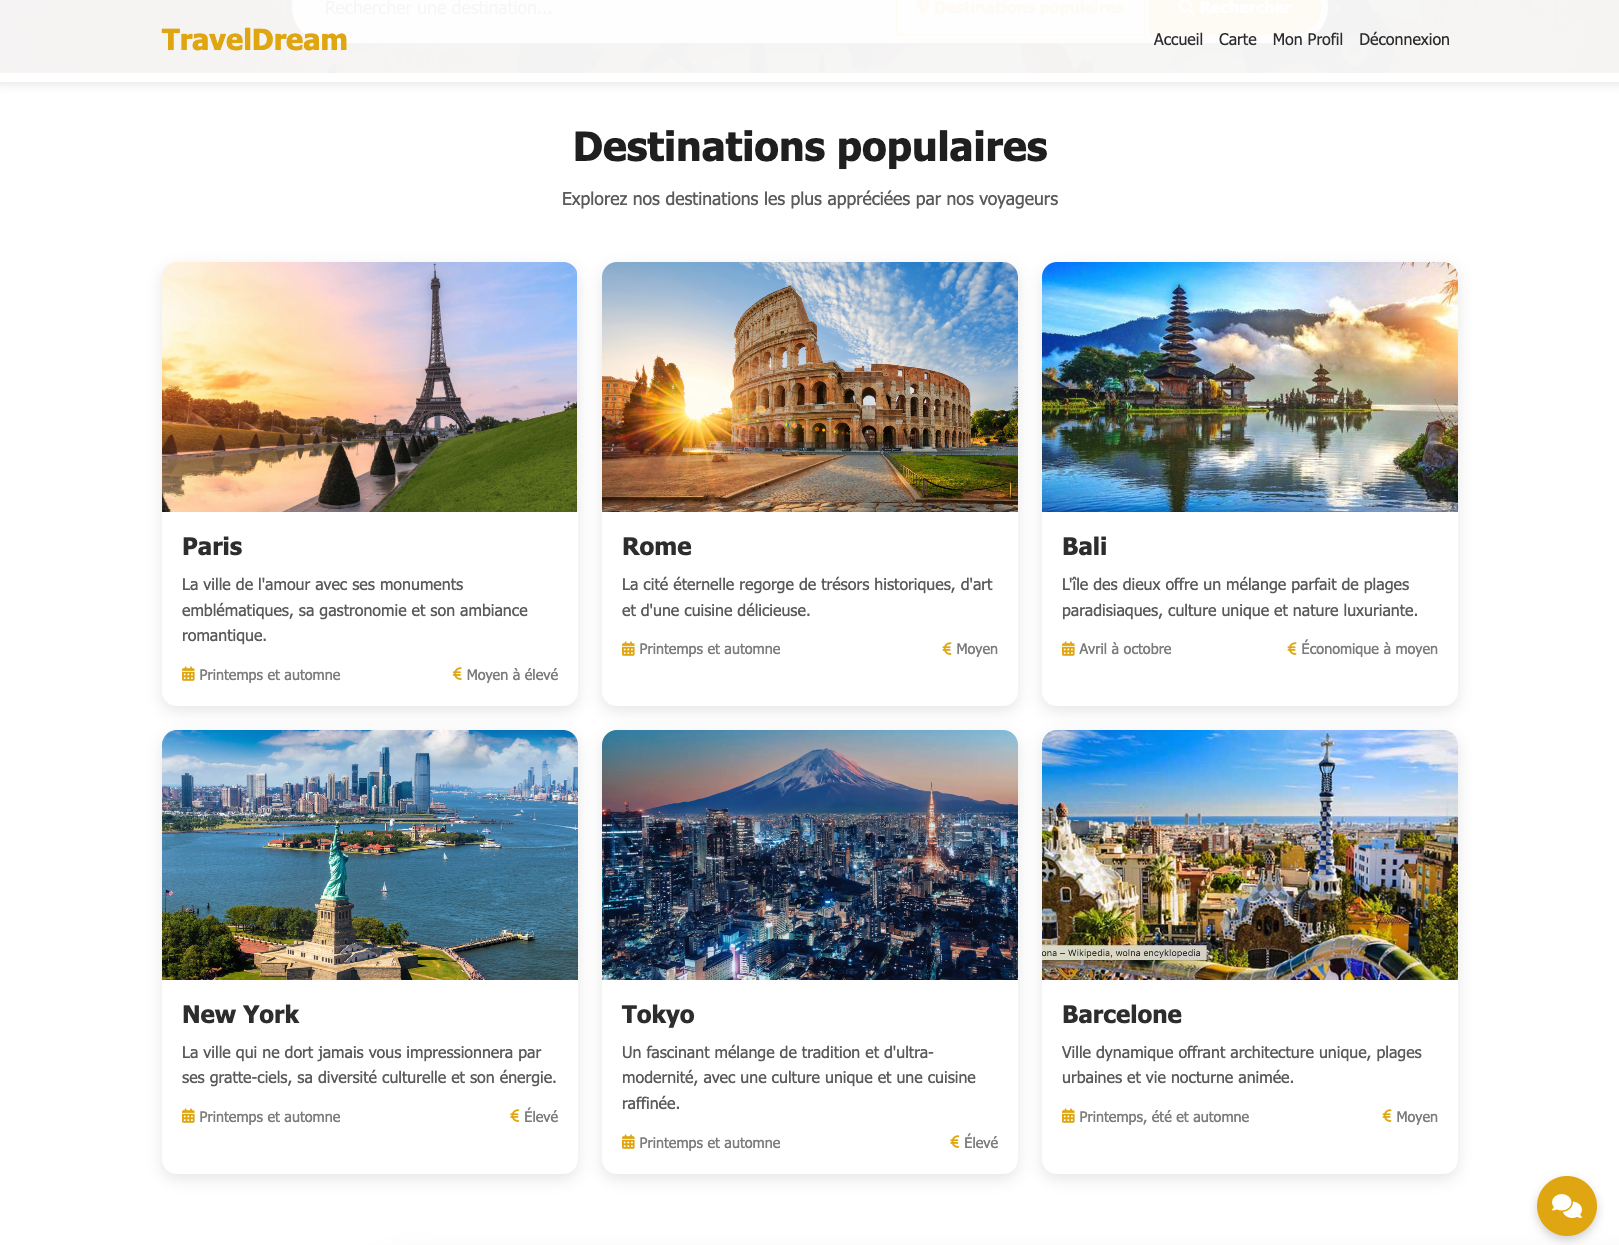
\includegraphics[width=0.8\textwidth]{4_accueil_1.png}
\end{figure}
\begin{figure}[H]
    \centering
    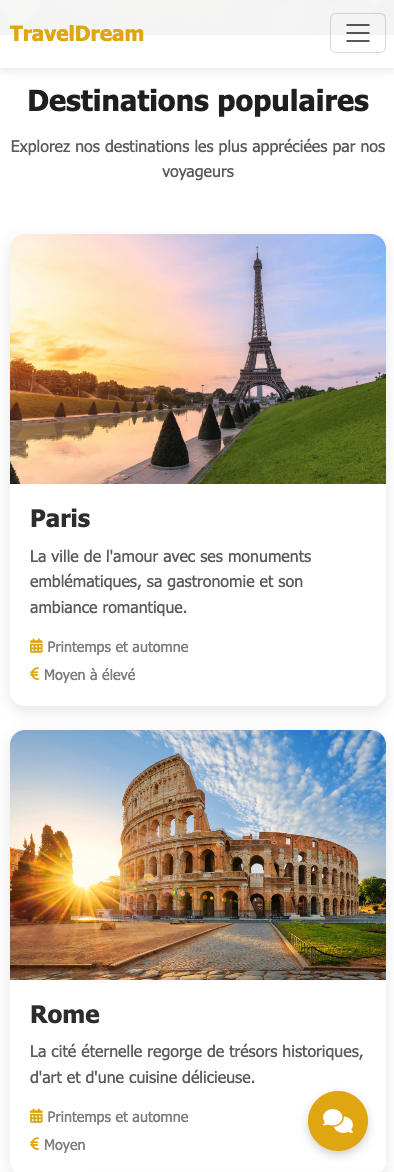
\includegraphics[width=0.4\textwidth]{4_accueil_2.png}
\end{figure}
\begin{figure}[H]
    \centering
    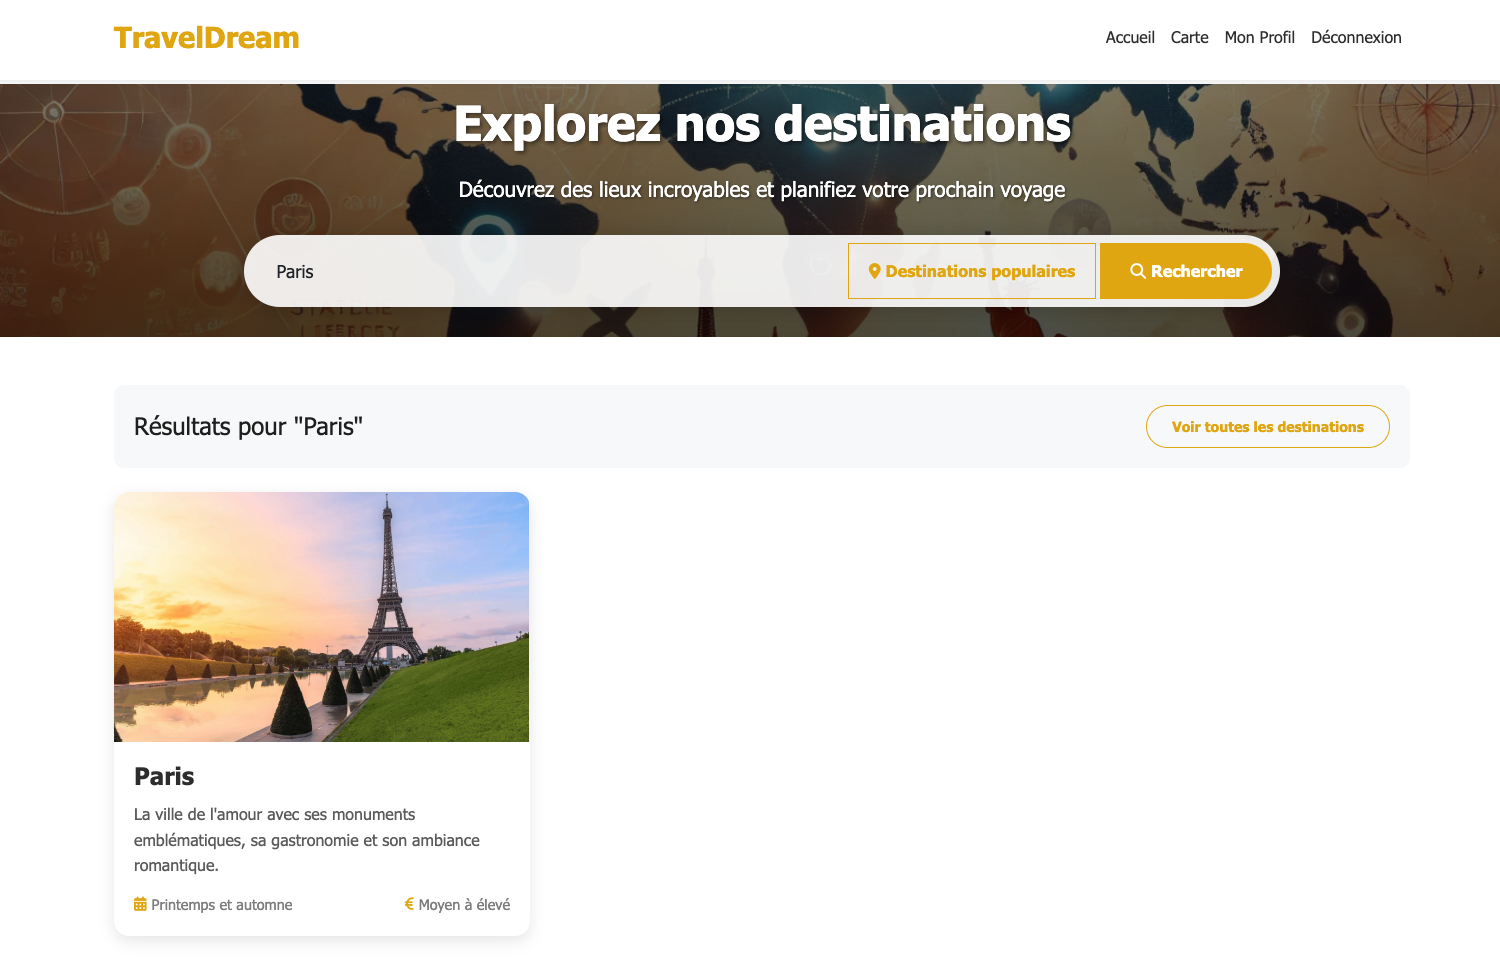
\includegraphics[width=0.8\textwidth]{4_accueil_3.png}
\end{figure}
\begin{figure}[H]
    \centering
    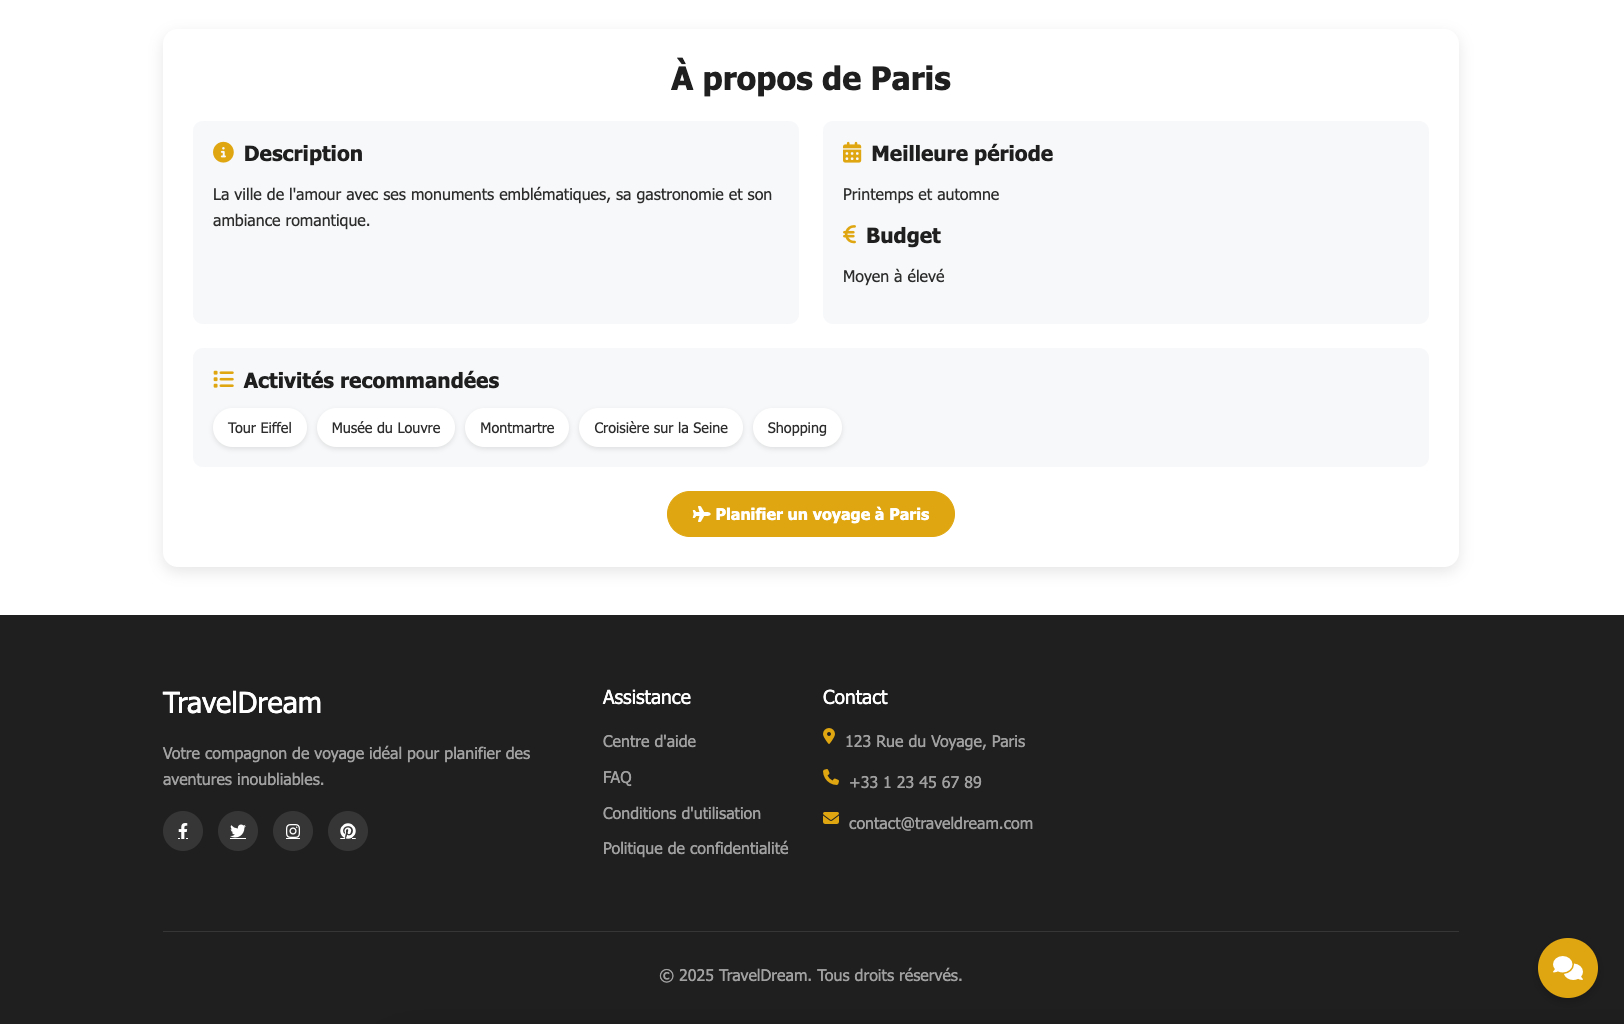
\includegraphics[width=0.8\textwidth]{4_accueil_4.png}
\end{figure}


\subsubsection{Carte des destinations}
Accessible en cliquant sur "Carte" dans la barre de navigation
\begin{figure}[H]
    \centering
    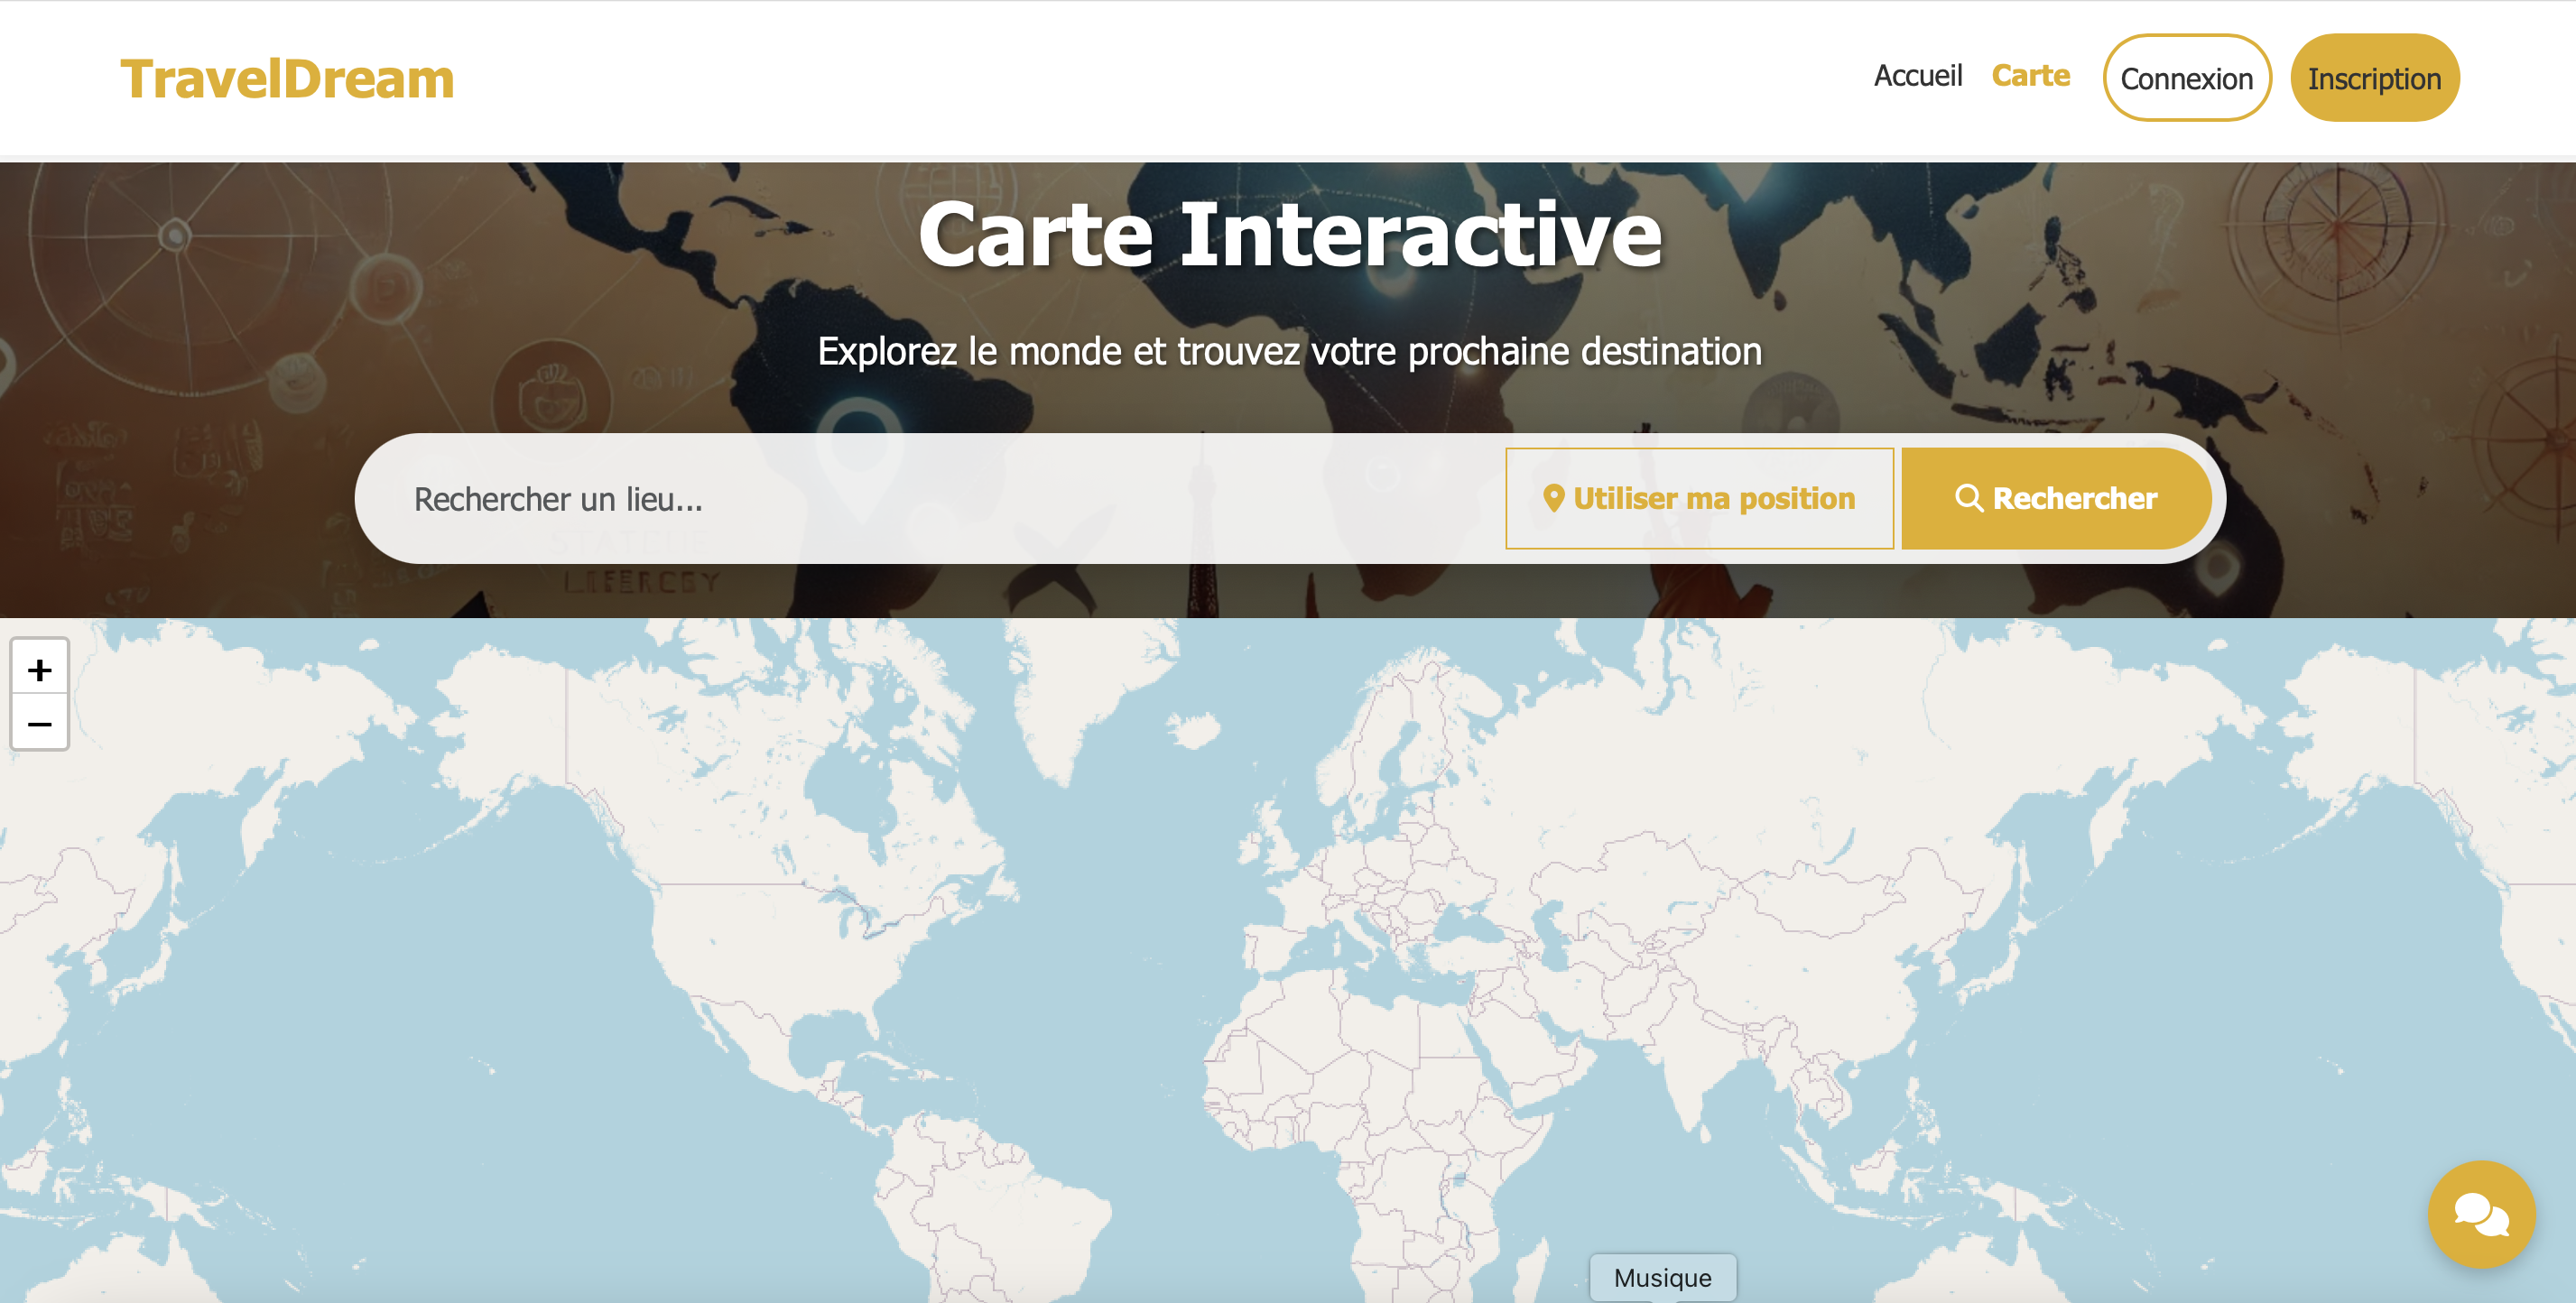
\includegraphics[width=0.8\textwidth]{5_carte_1.png}
\end{figure}
\begin{figure}[H]
    \centering
    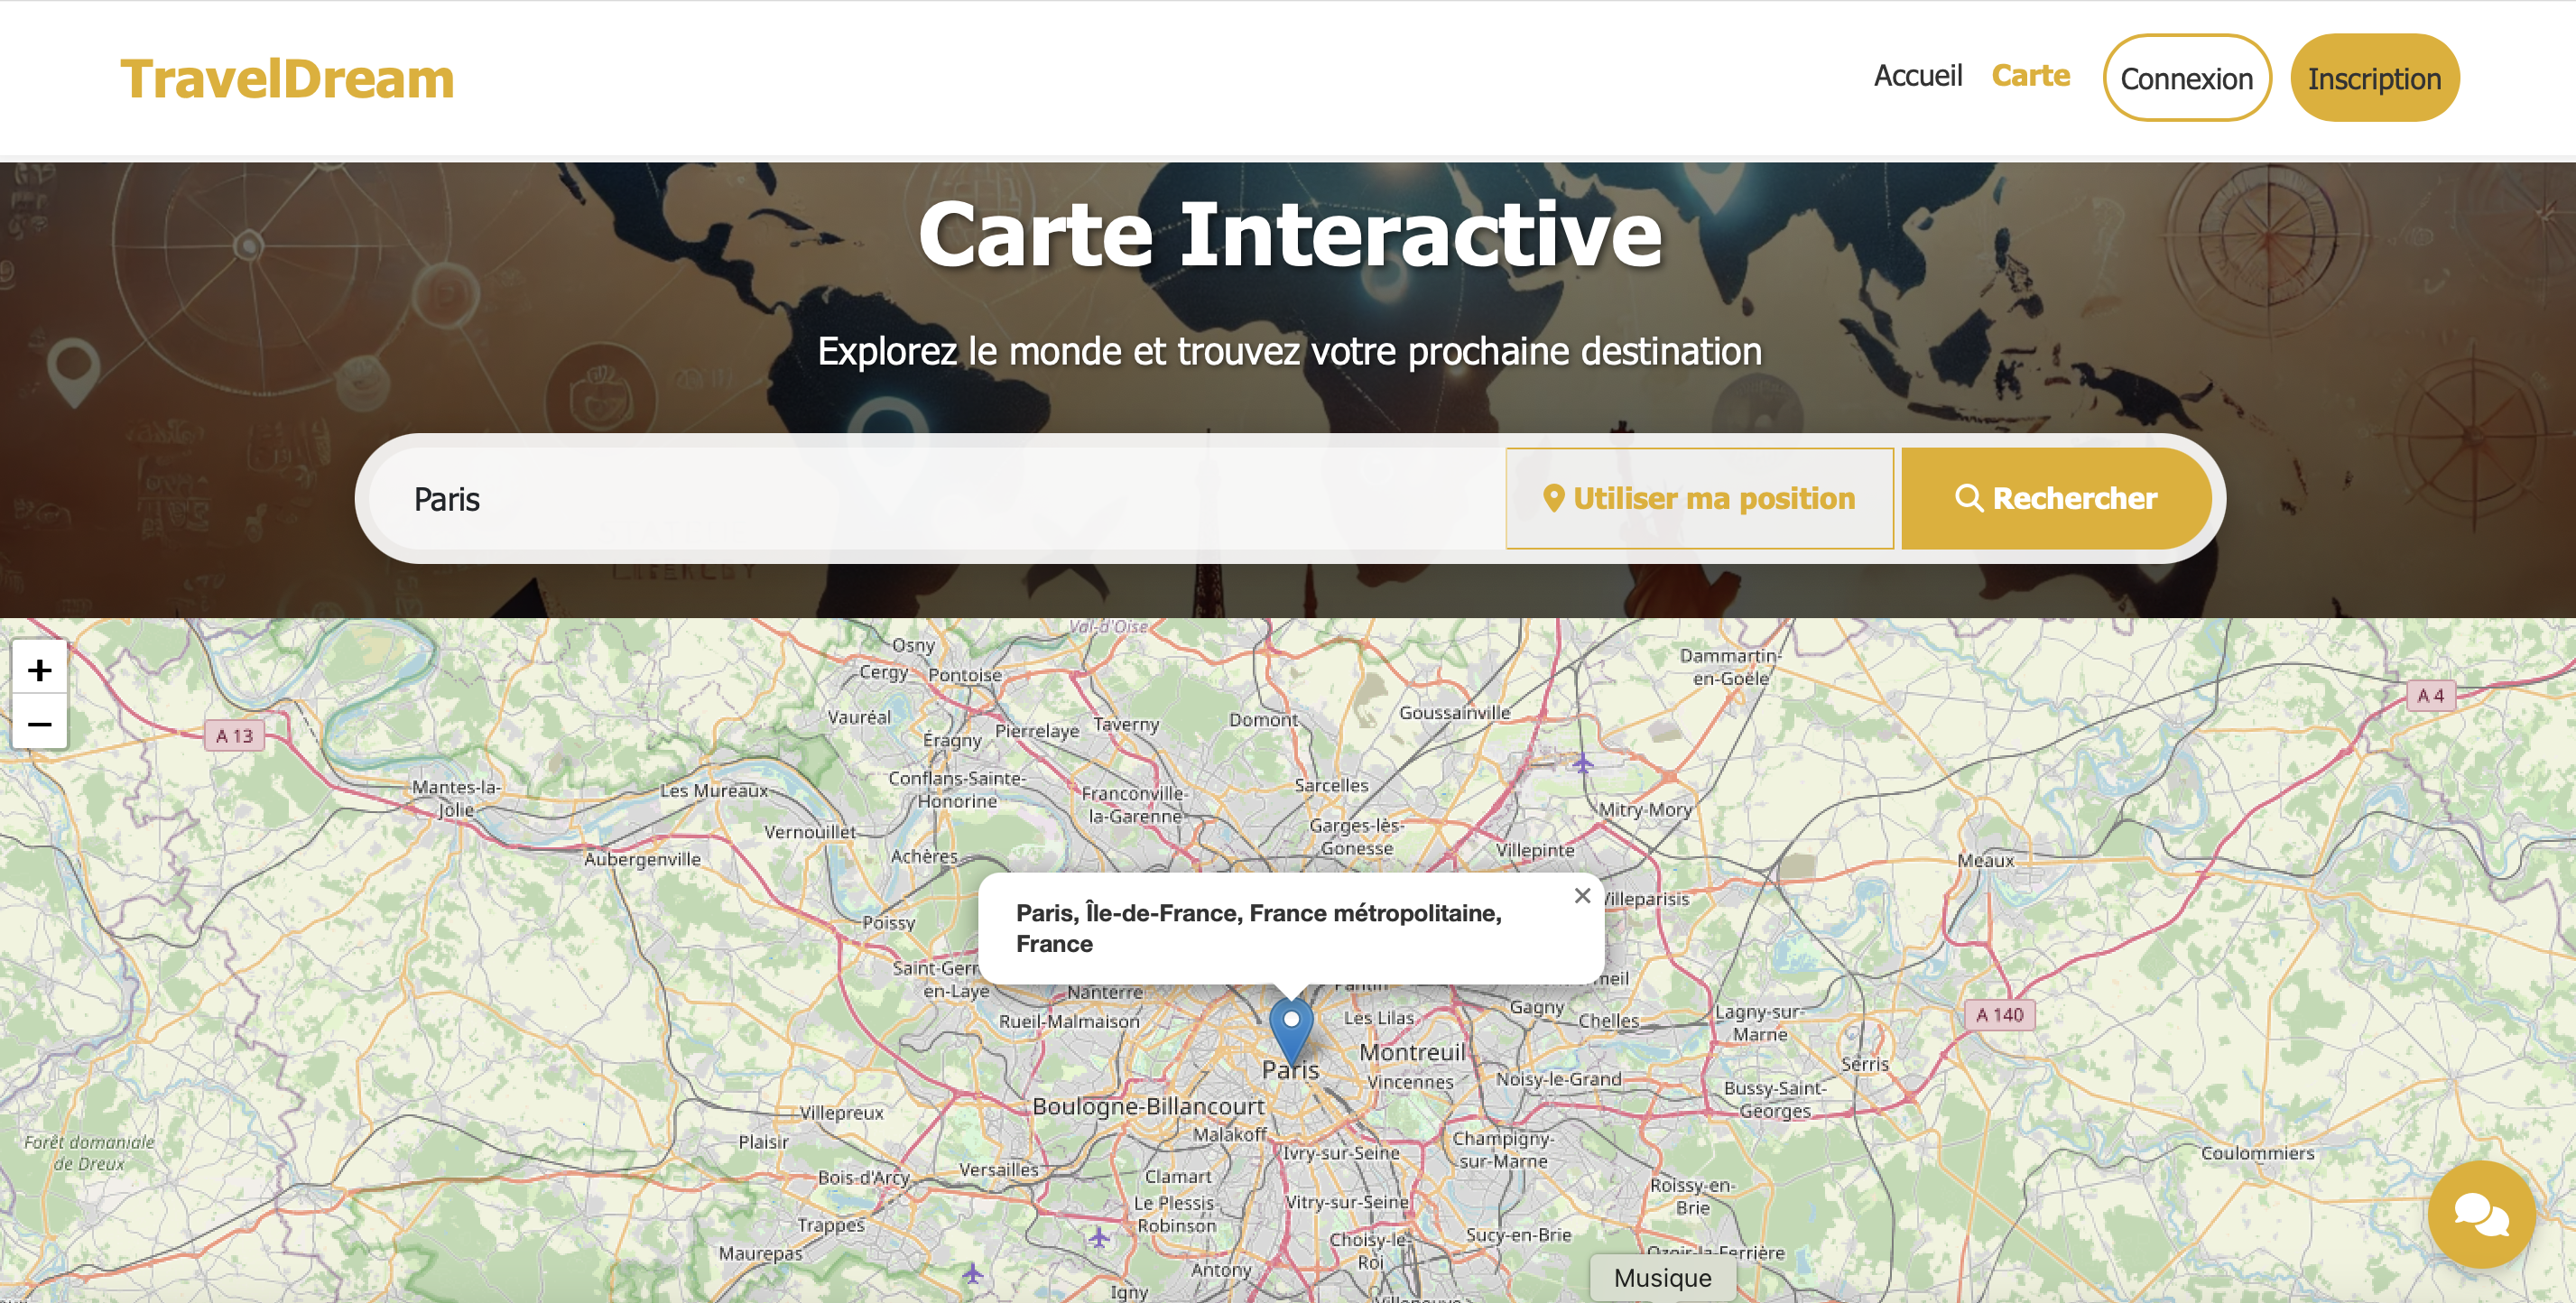
\includegraphics[width=0.8\textwidth]{5_carte_2.png}
\end{figure}



\subsection{Chatbot}
Accessible en cliquant sur la bulle en bas à droite (qui apparait après la page de connexion) 
\begin{figure}[H]
    \centering
    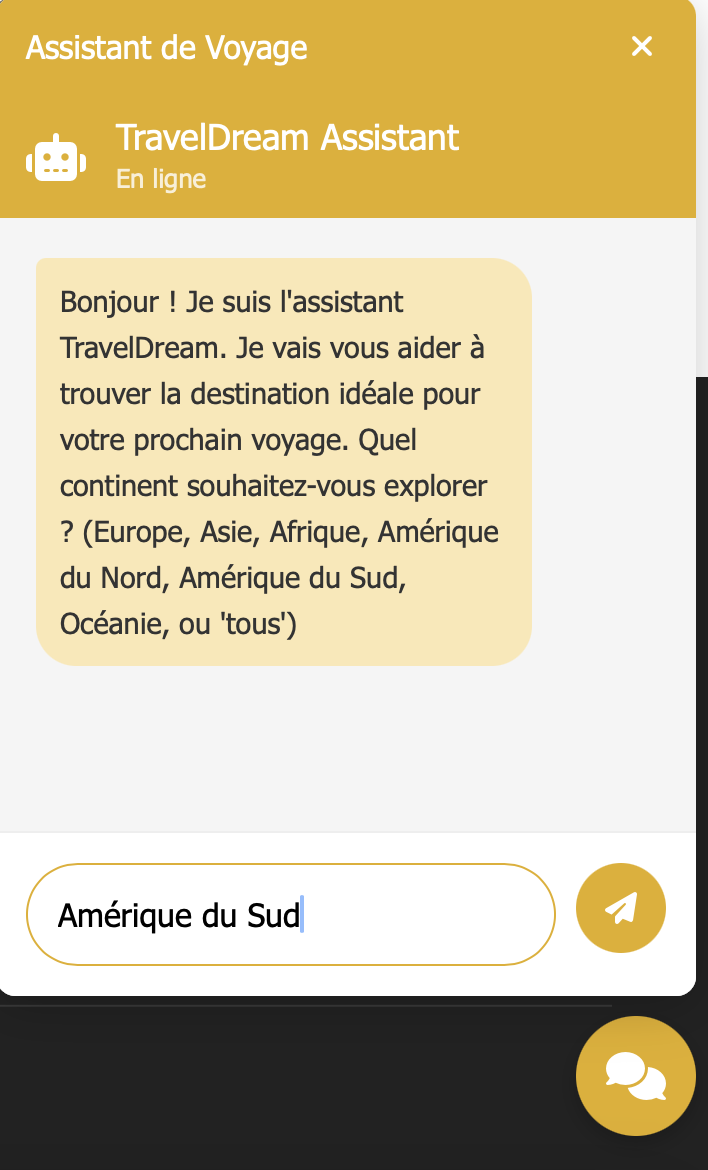
\includegraphics[width=0.4\textwidth]{6_chatbot_1.png}
\end{figure}
\begin{figure}[H]
    \centering
    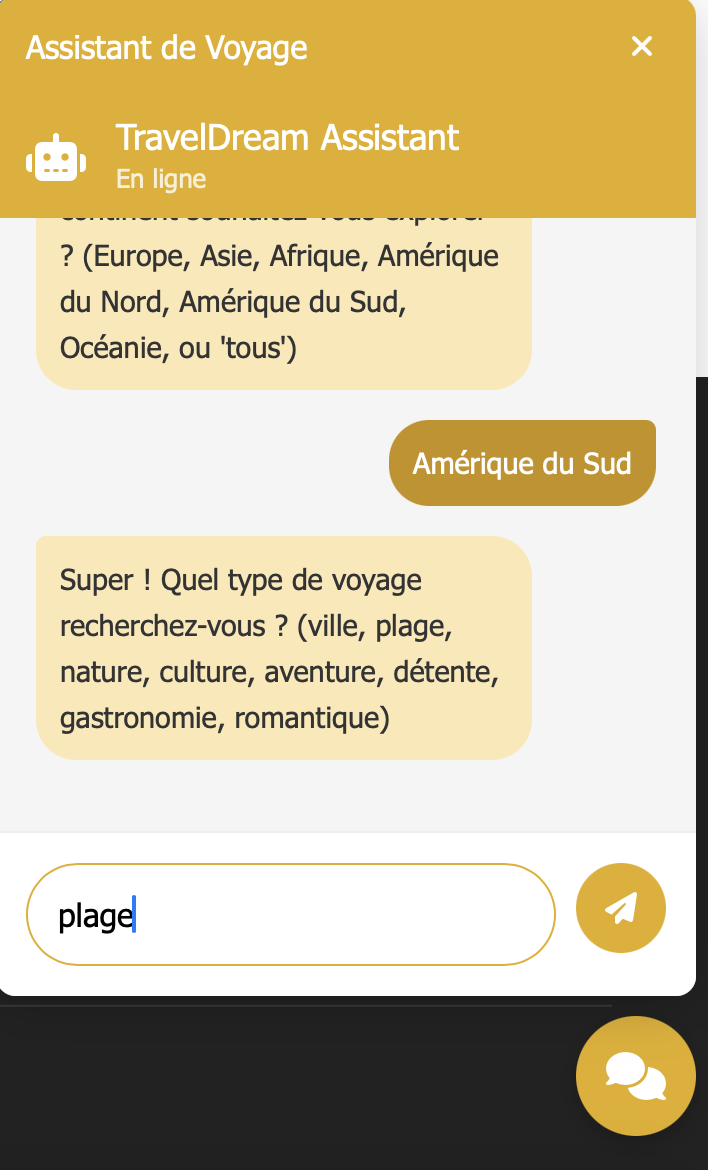
\includegraphics[width=0.4\textwidth]{6_chatbot_2.png}
\end{figure}
\begin{figure}[H]
    \centering
    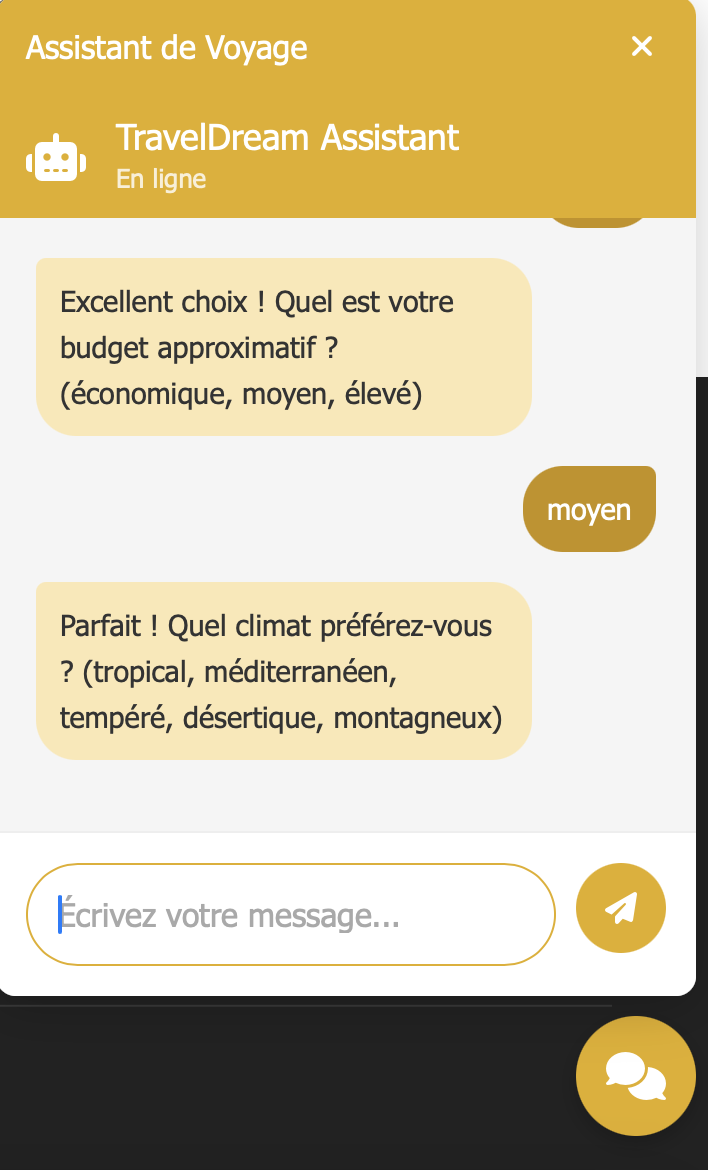
\includegraphics[width=0.4\textwidth]{6_chatbot_3.png}
\end{figure}
\begin{figure}[H]
    \centering
    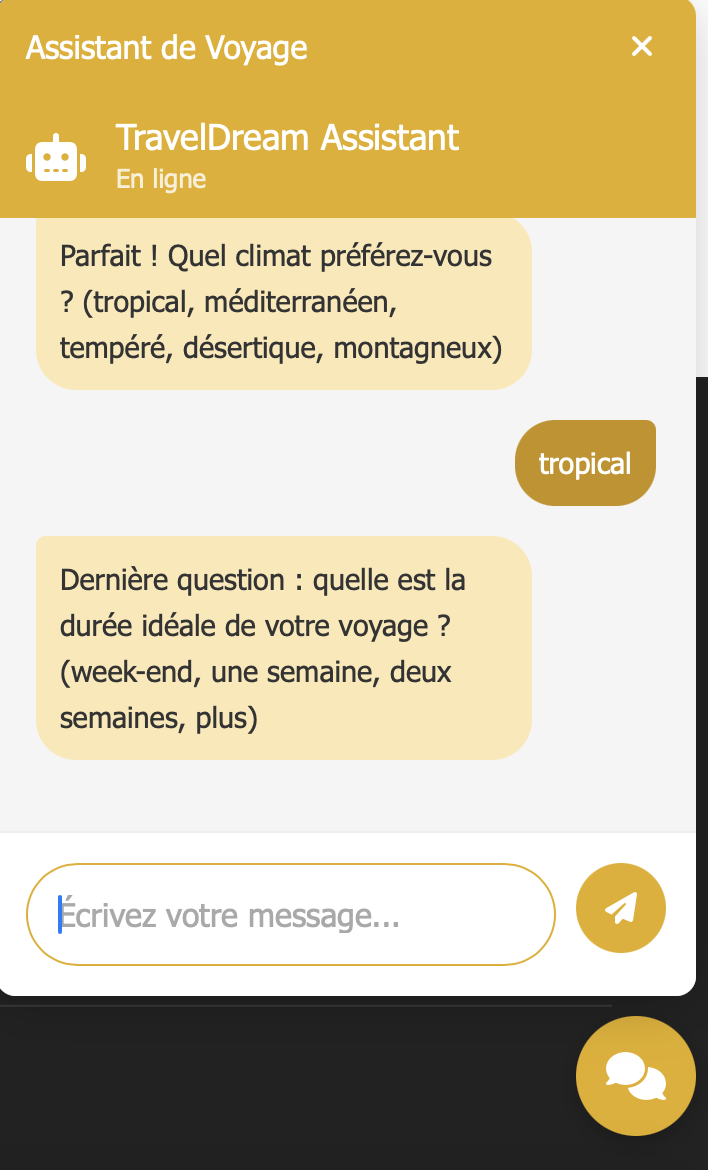
\includegraphics[width=0.4\textwidth]{6_chatbot_4.png}
\end{figure}
\begin{figure}[H]
    \centering
    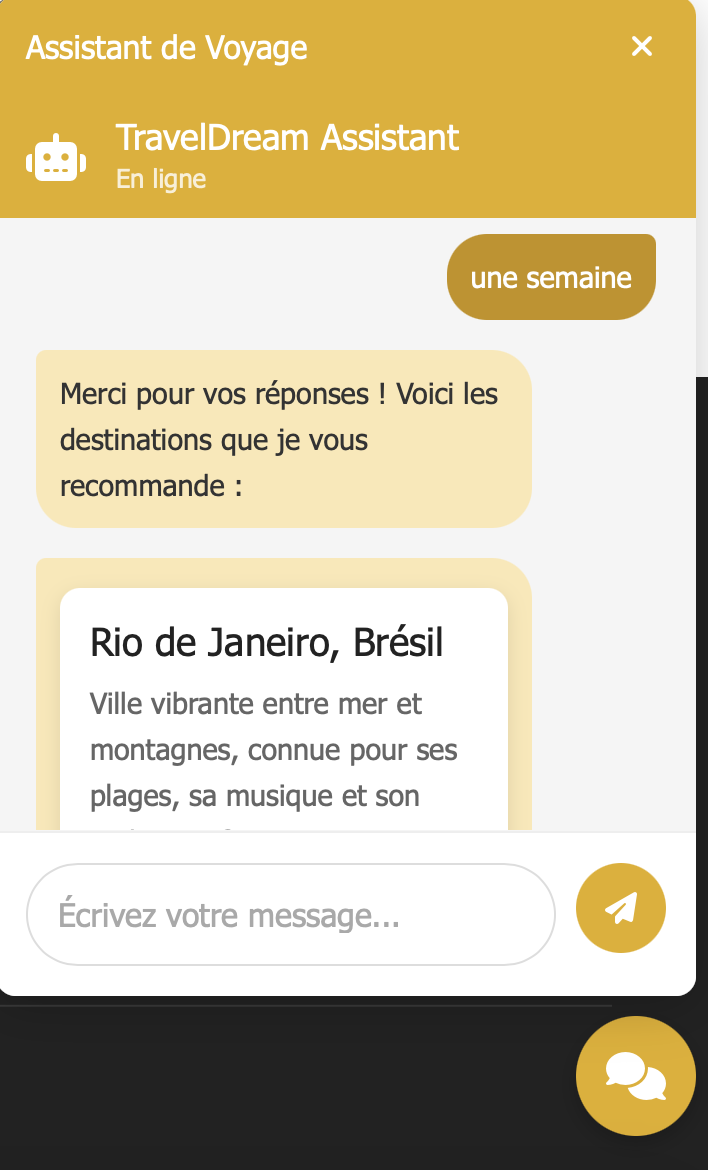
\includegraphics[width=0.4\textwidth]{6_chatbot_5.png}
\end{figure}
\begin{figure}[H]
    \centering
    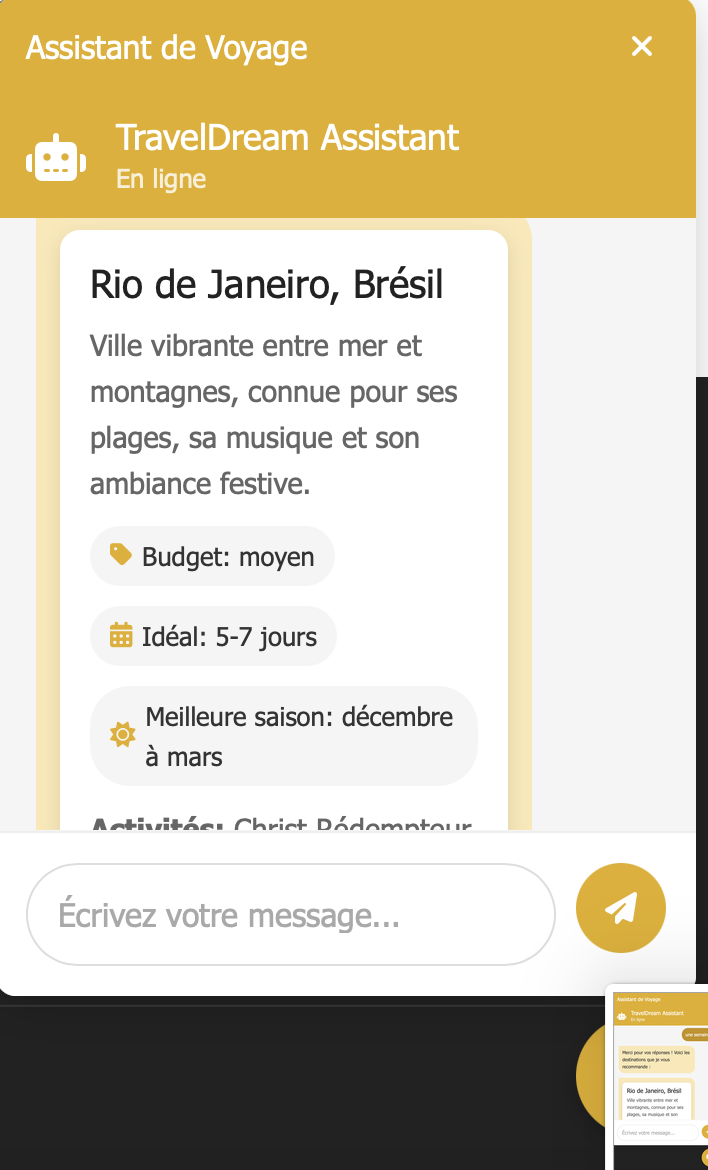
\includegraphics[width=0.4\textwidth]{6_chatbot_6.png}
\end{figure}
\begin{figure}[H]
    \centering
    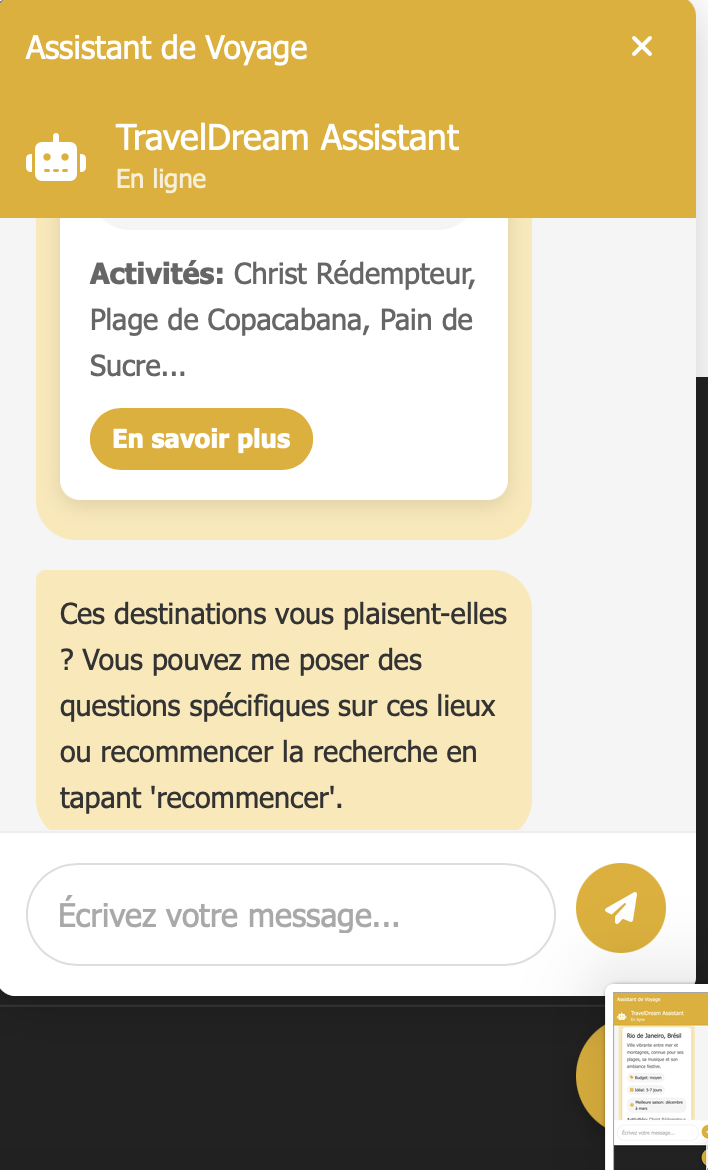
\includegraphics[width=0.4\textwidth]{6_chatbot_7.png}
\end{figure}

\subsection{Gestion des voyages}

\subsubsection{Profil et liste des voyages}
Accessible en cliquant sur "Mon profil" dans la barre de navigation
\begin{figure}[H]
    \centering
    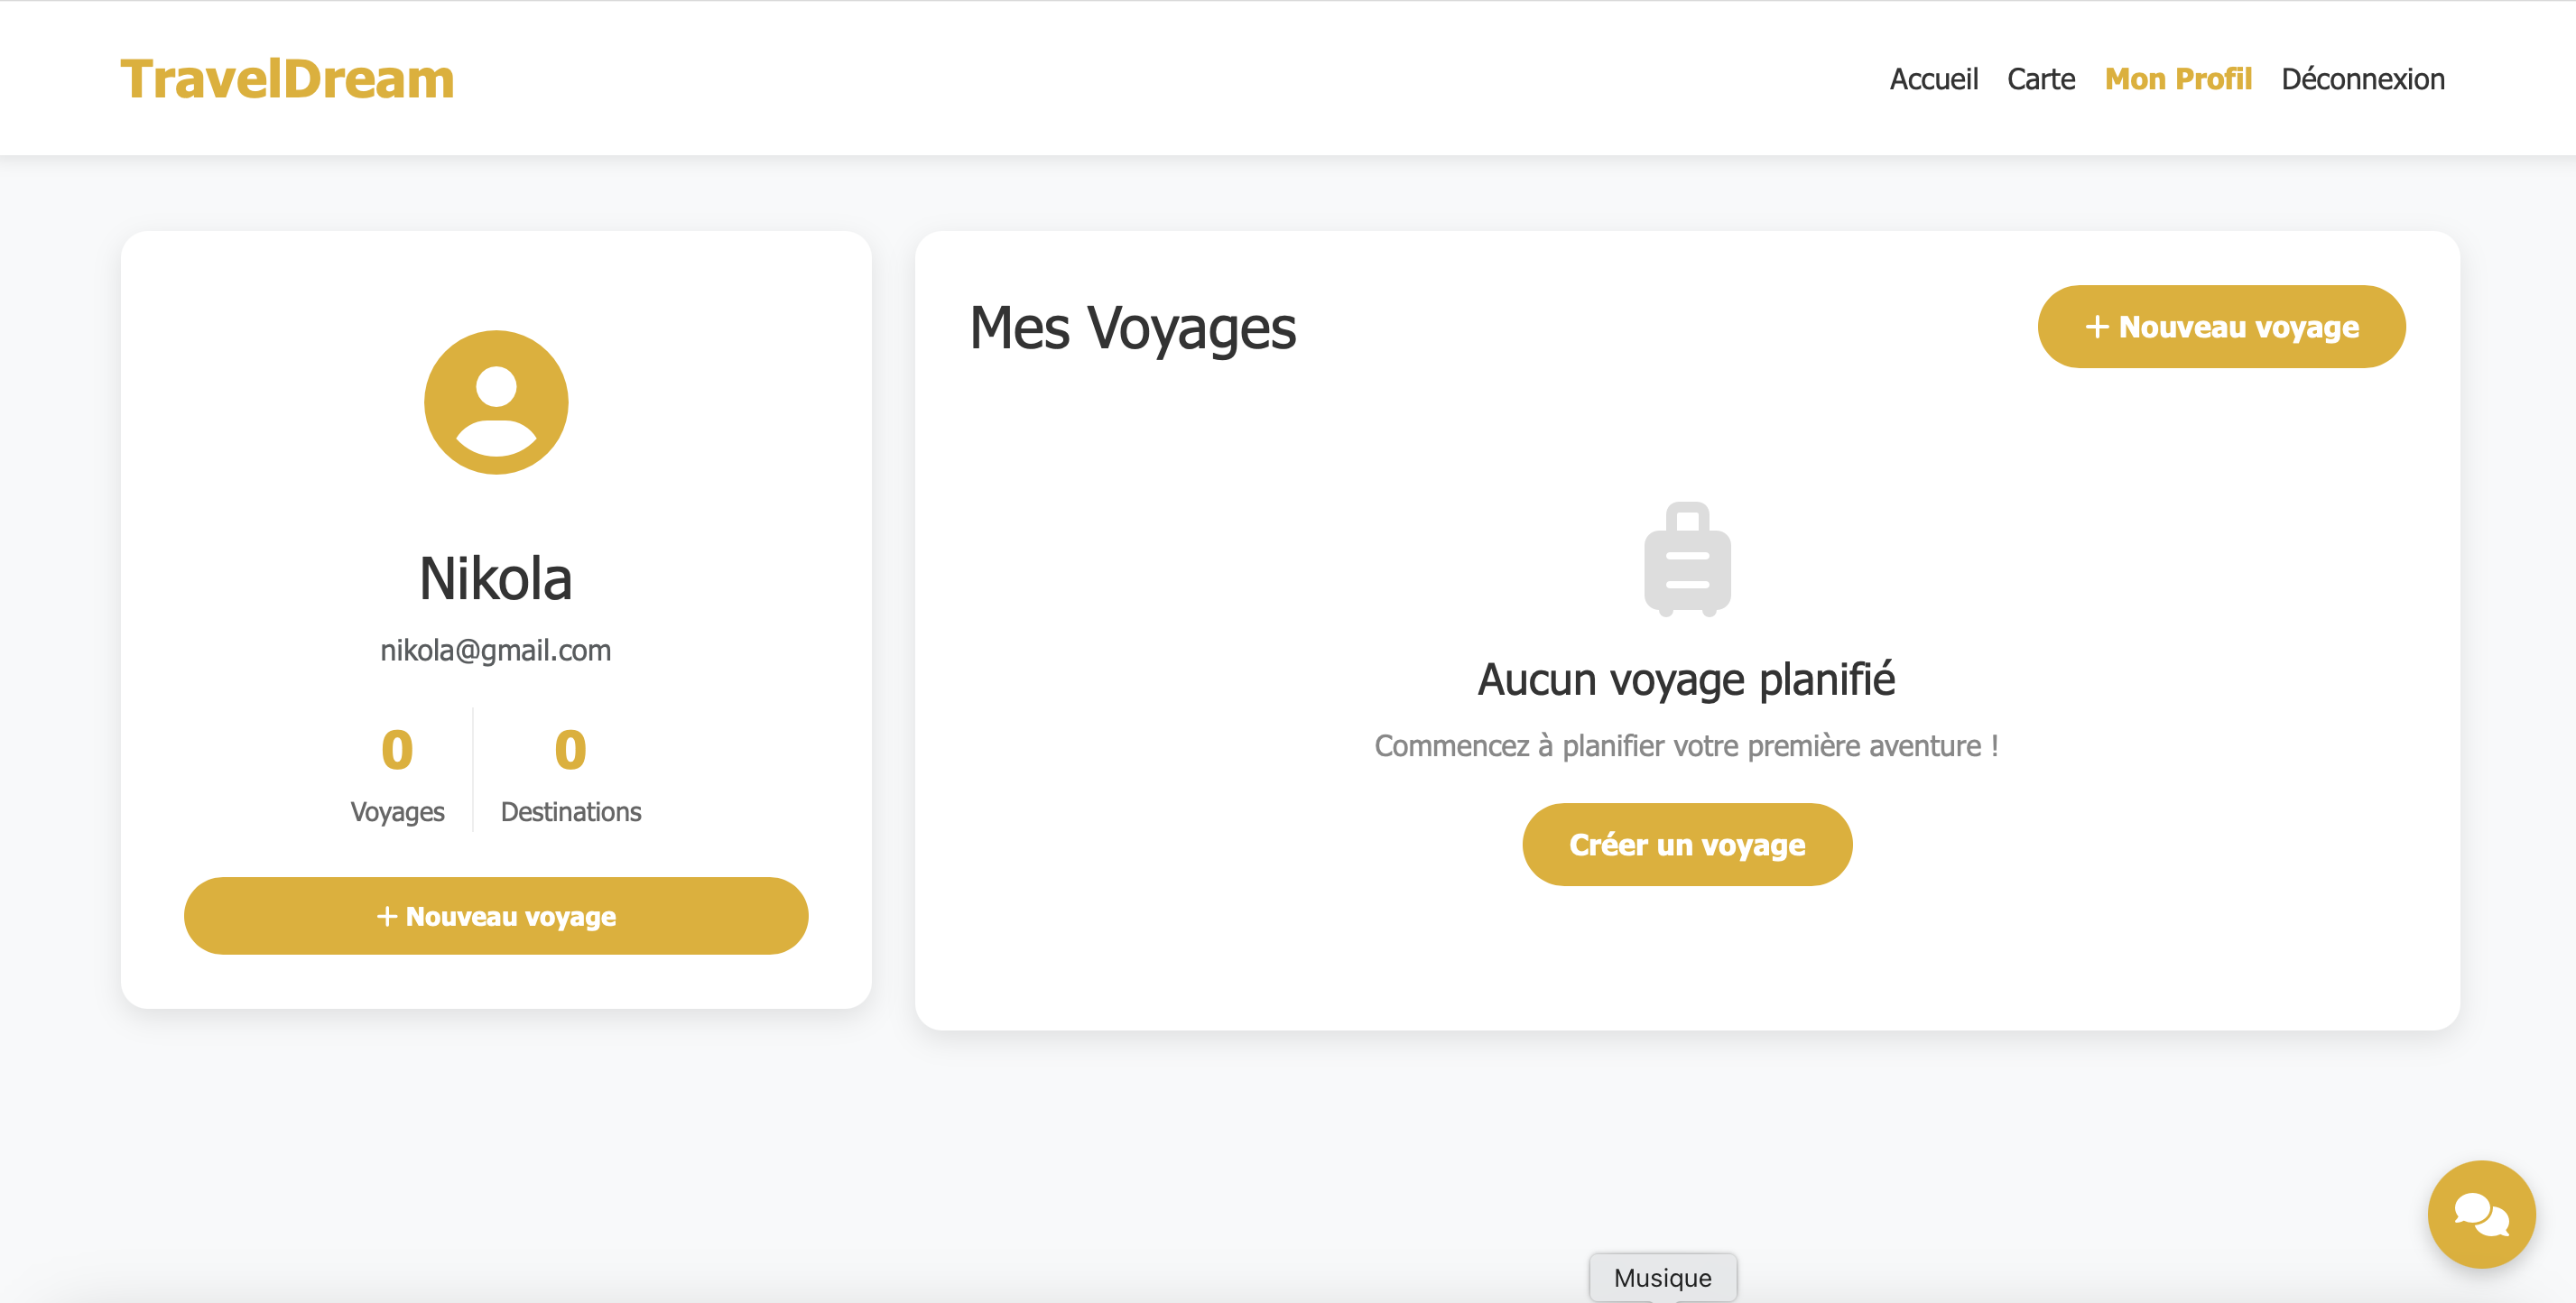
\includegraphics[width=0.8\textwidth]{7_profil_voyage.png}
\end{figure}
\begin{figure}[H]
    \centering
    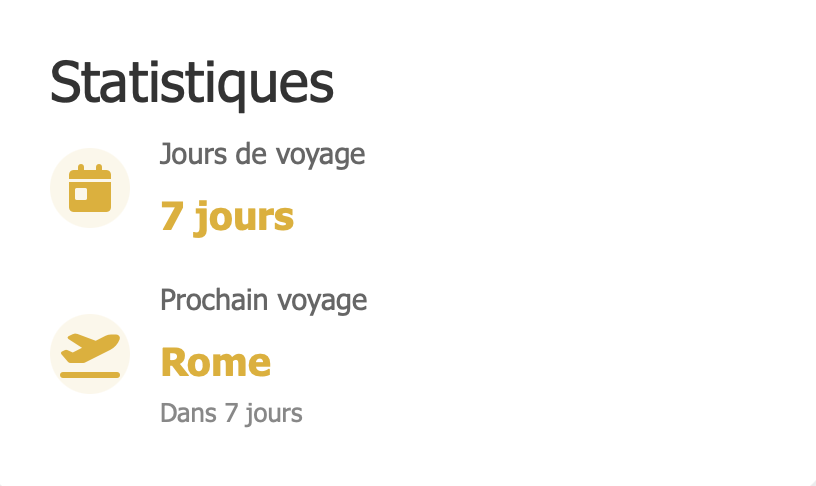
\includegraphics[width=0.8\textwidth]{7_profil_voyage_stats.png}
\end{figure}


\subsubsection{Ajouter ou modifier un voyage}
Accessible en cliquant sur "Créer un voyage" depuis "Mon profil" et d'autres endroits dans l'application\\
Accessible en cliquant sur "Modifier" depuis "Mon profil" à partir d'un voyage déjà créé ou "Modifier" à partir des détails du voyage
\begin{figure}[H]
    \centering
    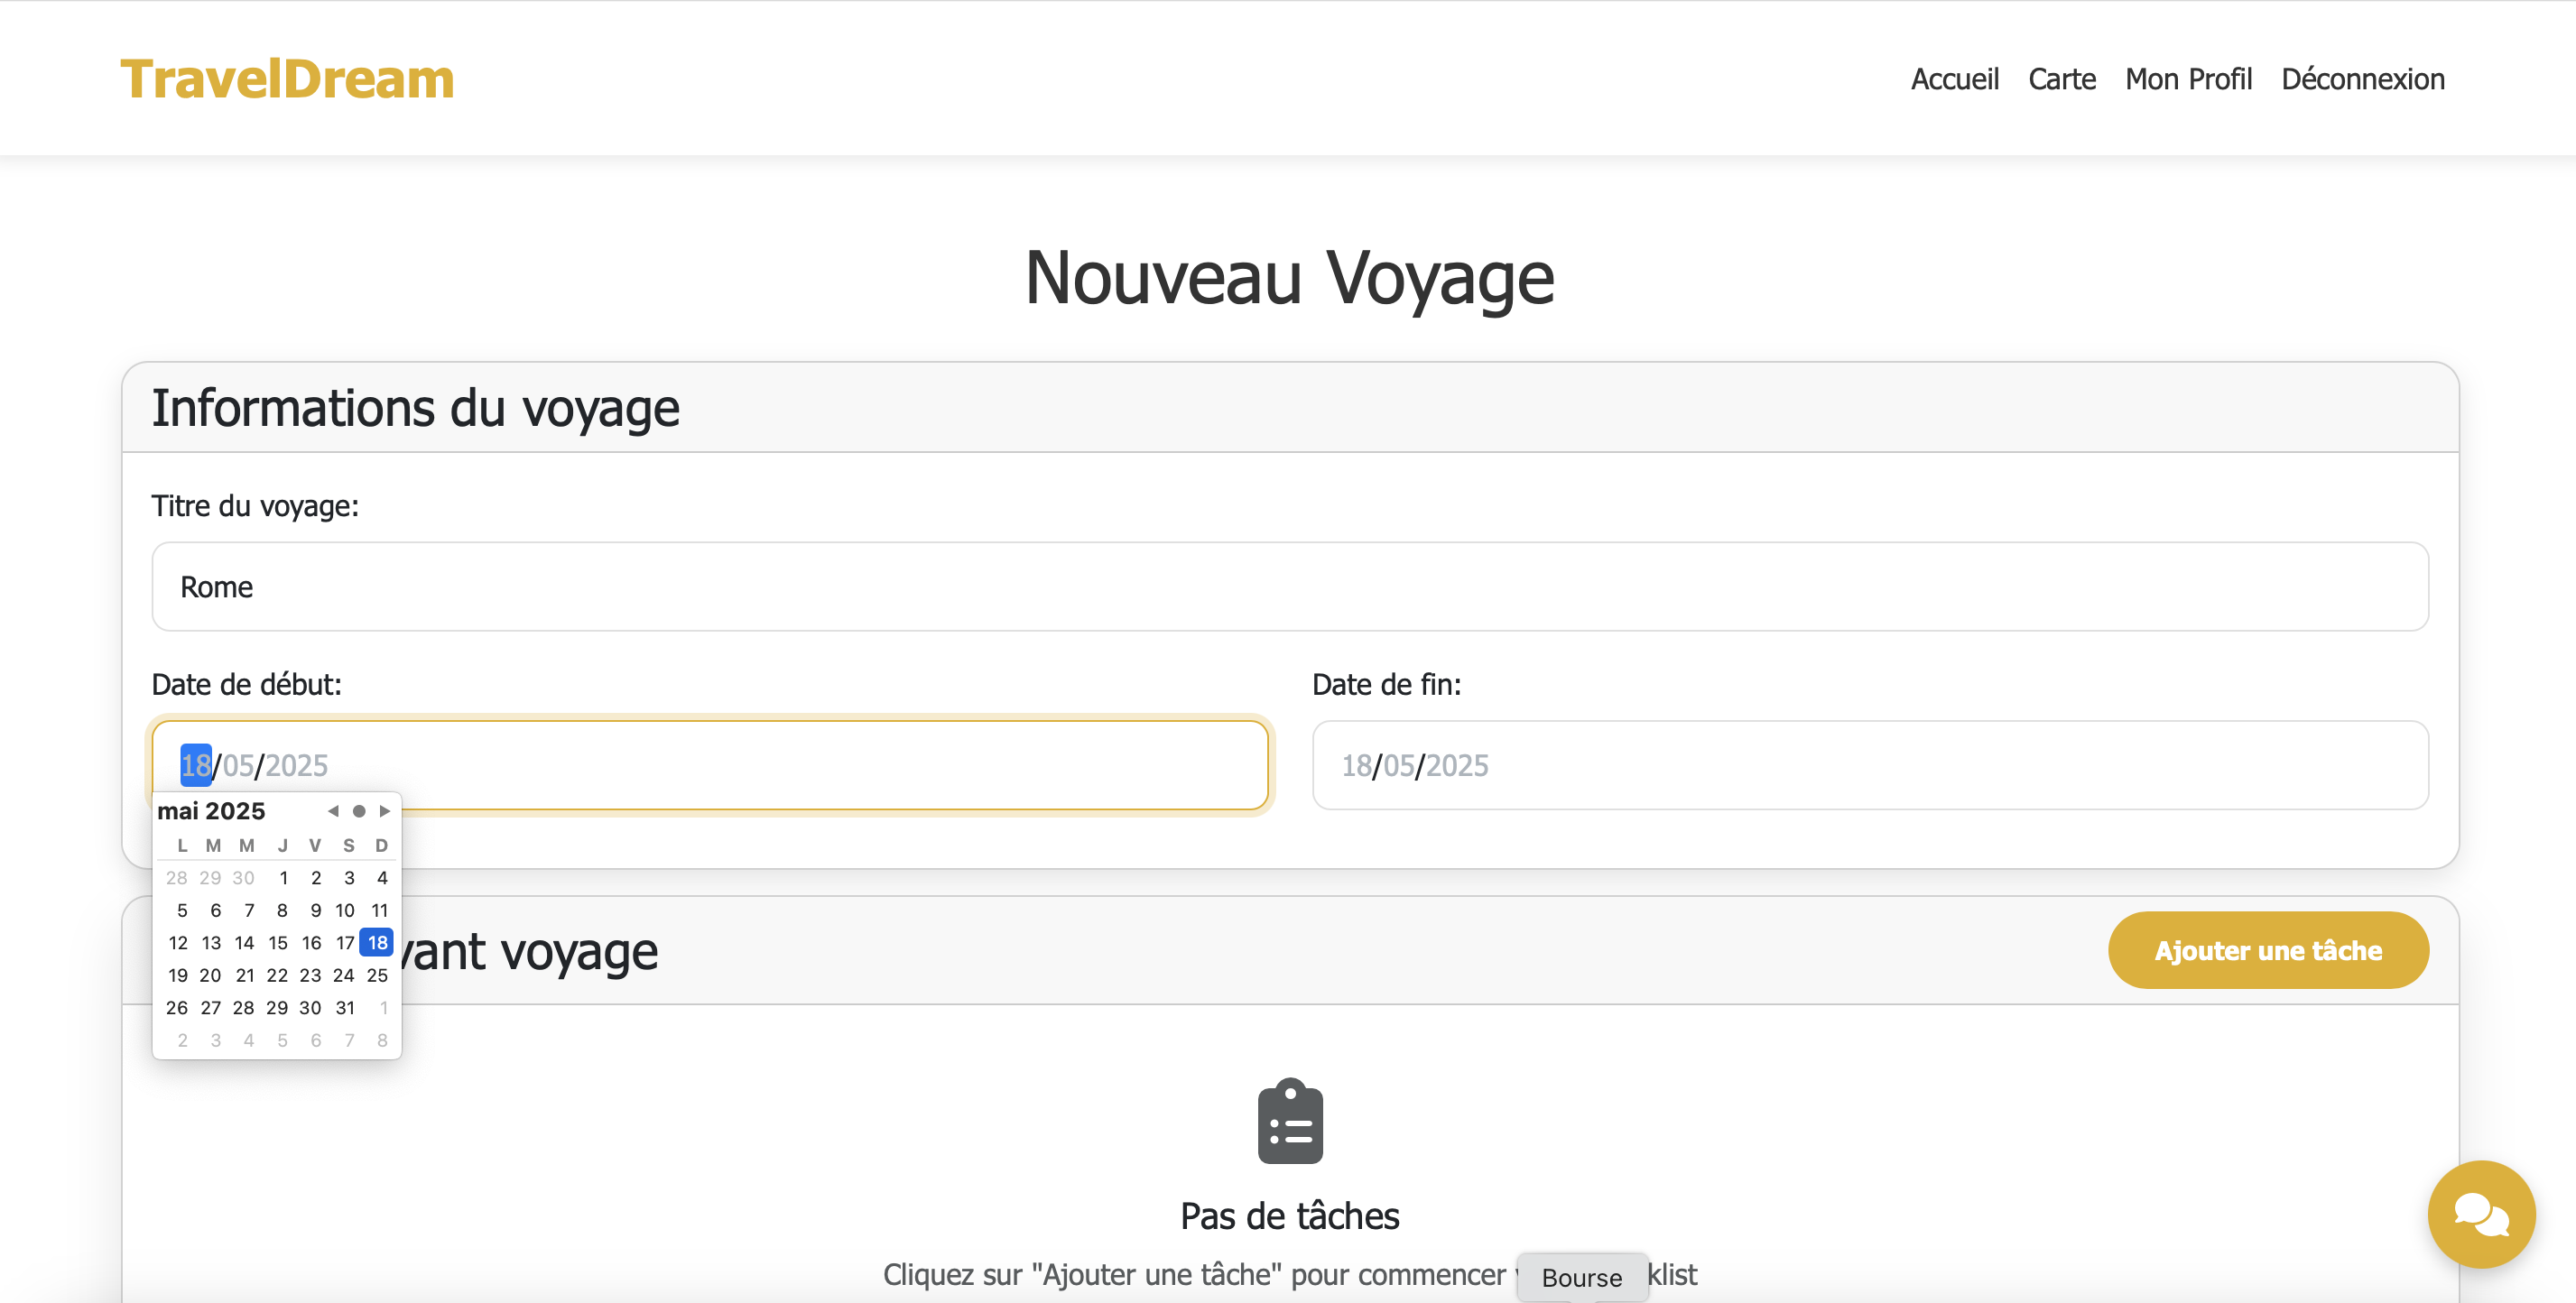
\includegraphics[width=0.8\textwidth]{8_creation_voyage_1.png}
\end{figure}
\begin{figure}[H]
    \centering
    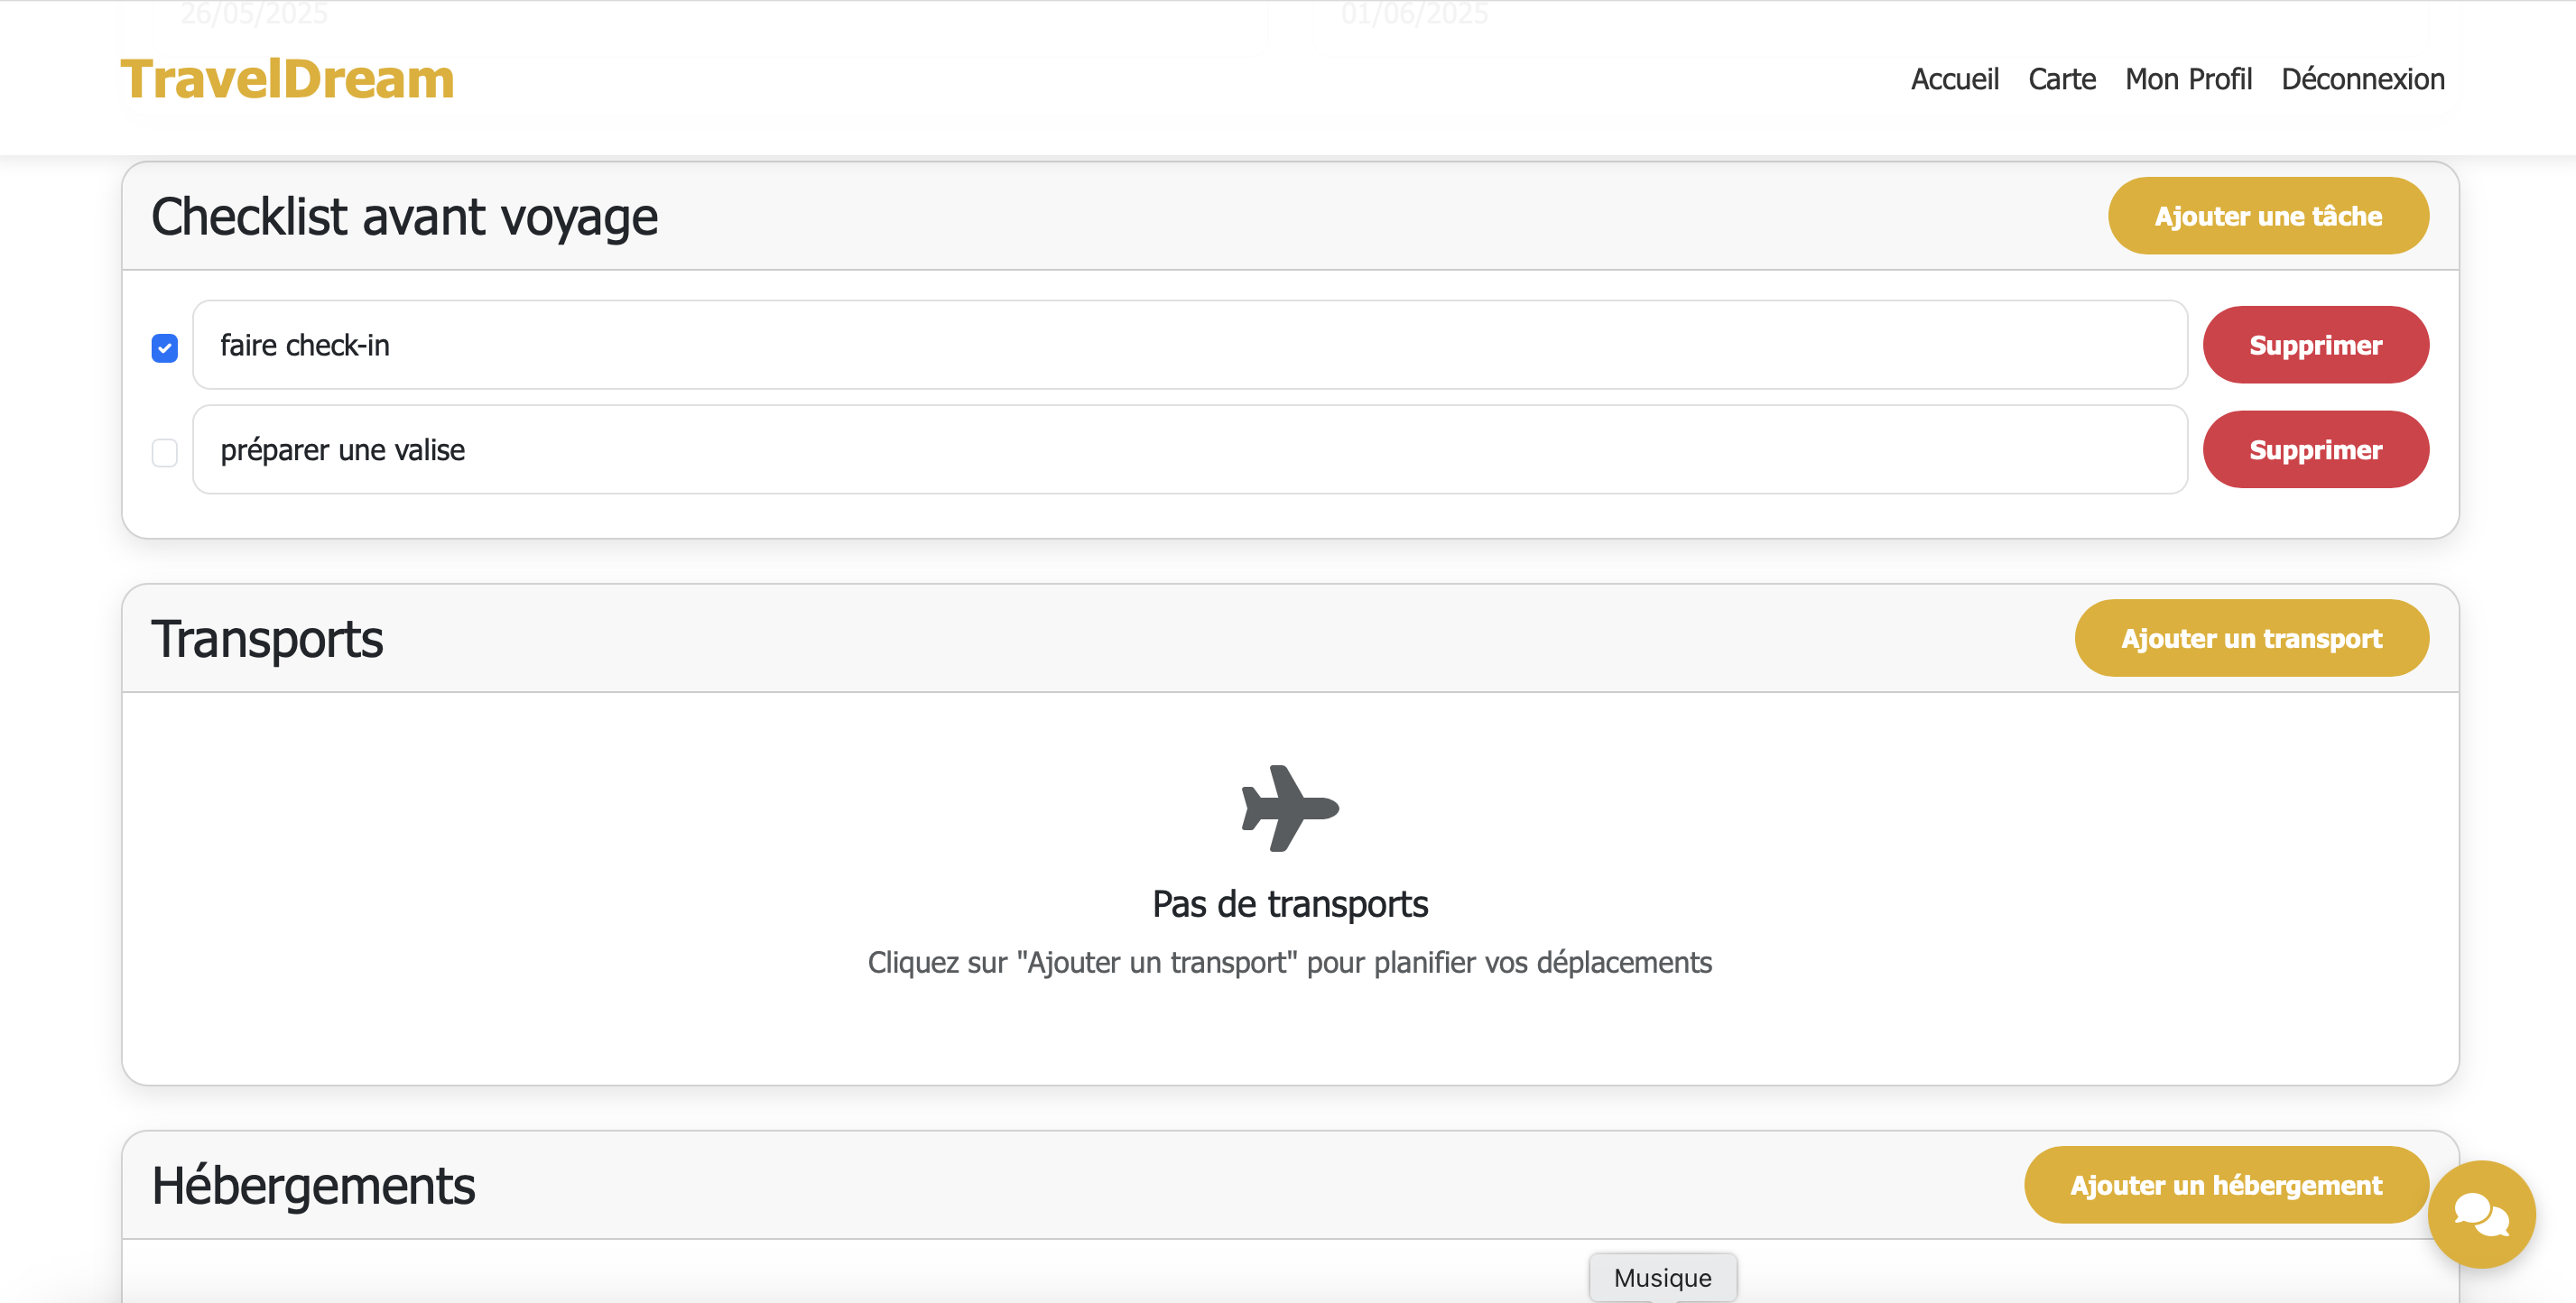
\includegraphics[width=0.8\textwidth]{8_creation_voyage_2.png}
\end{figure}
\begin{figure}[H]
    \centering
    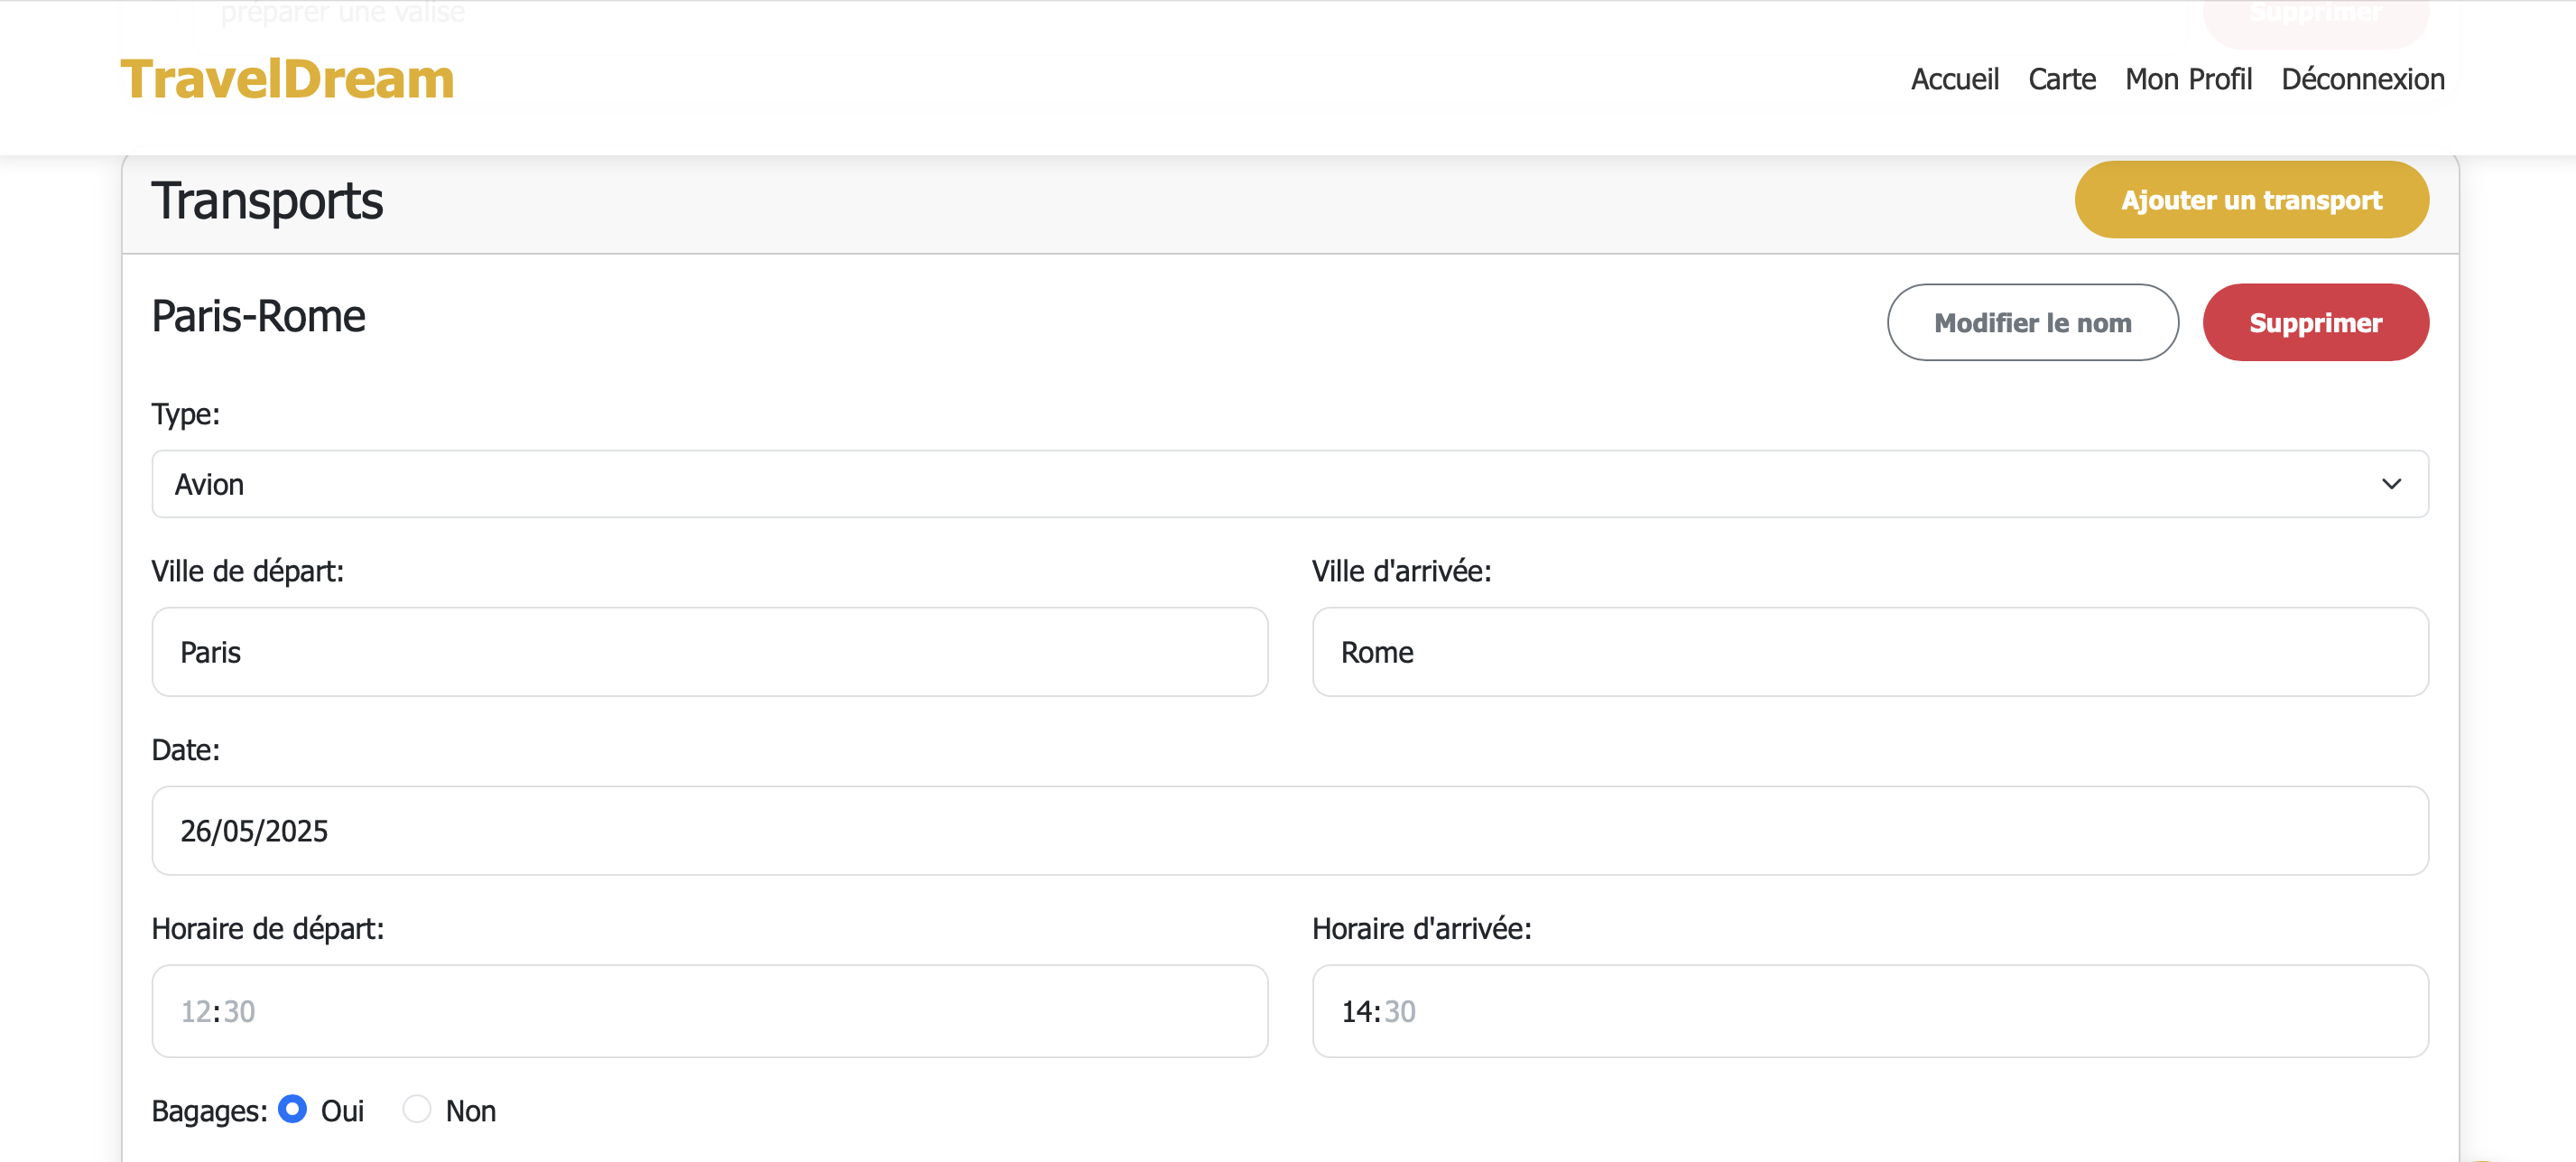
\includegraphics[width=0.8\textwidth]{8_creation_voyage_3.png}
\end{figure}
\begin{figure}[H]
    \centering
    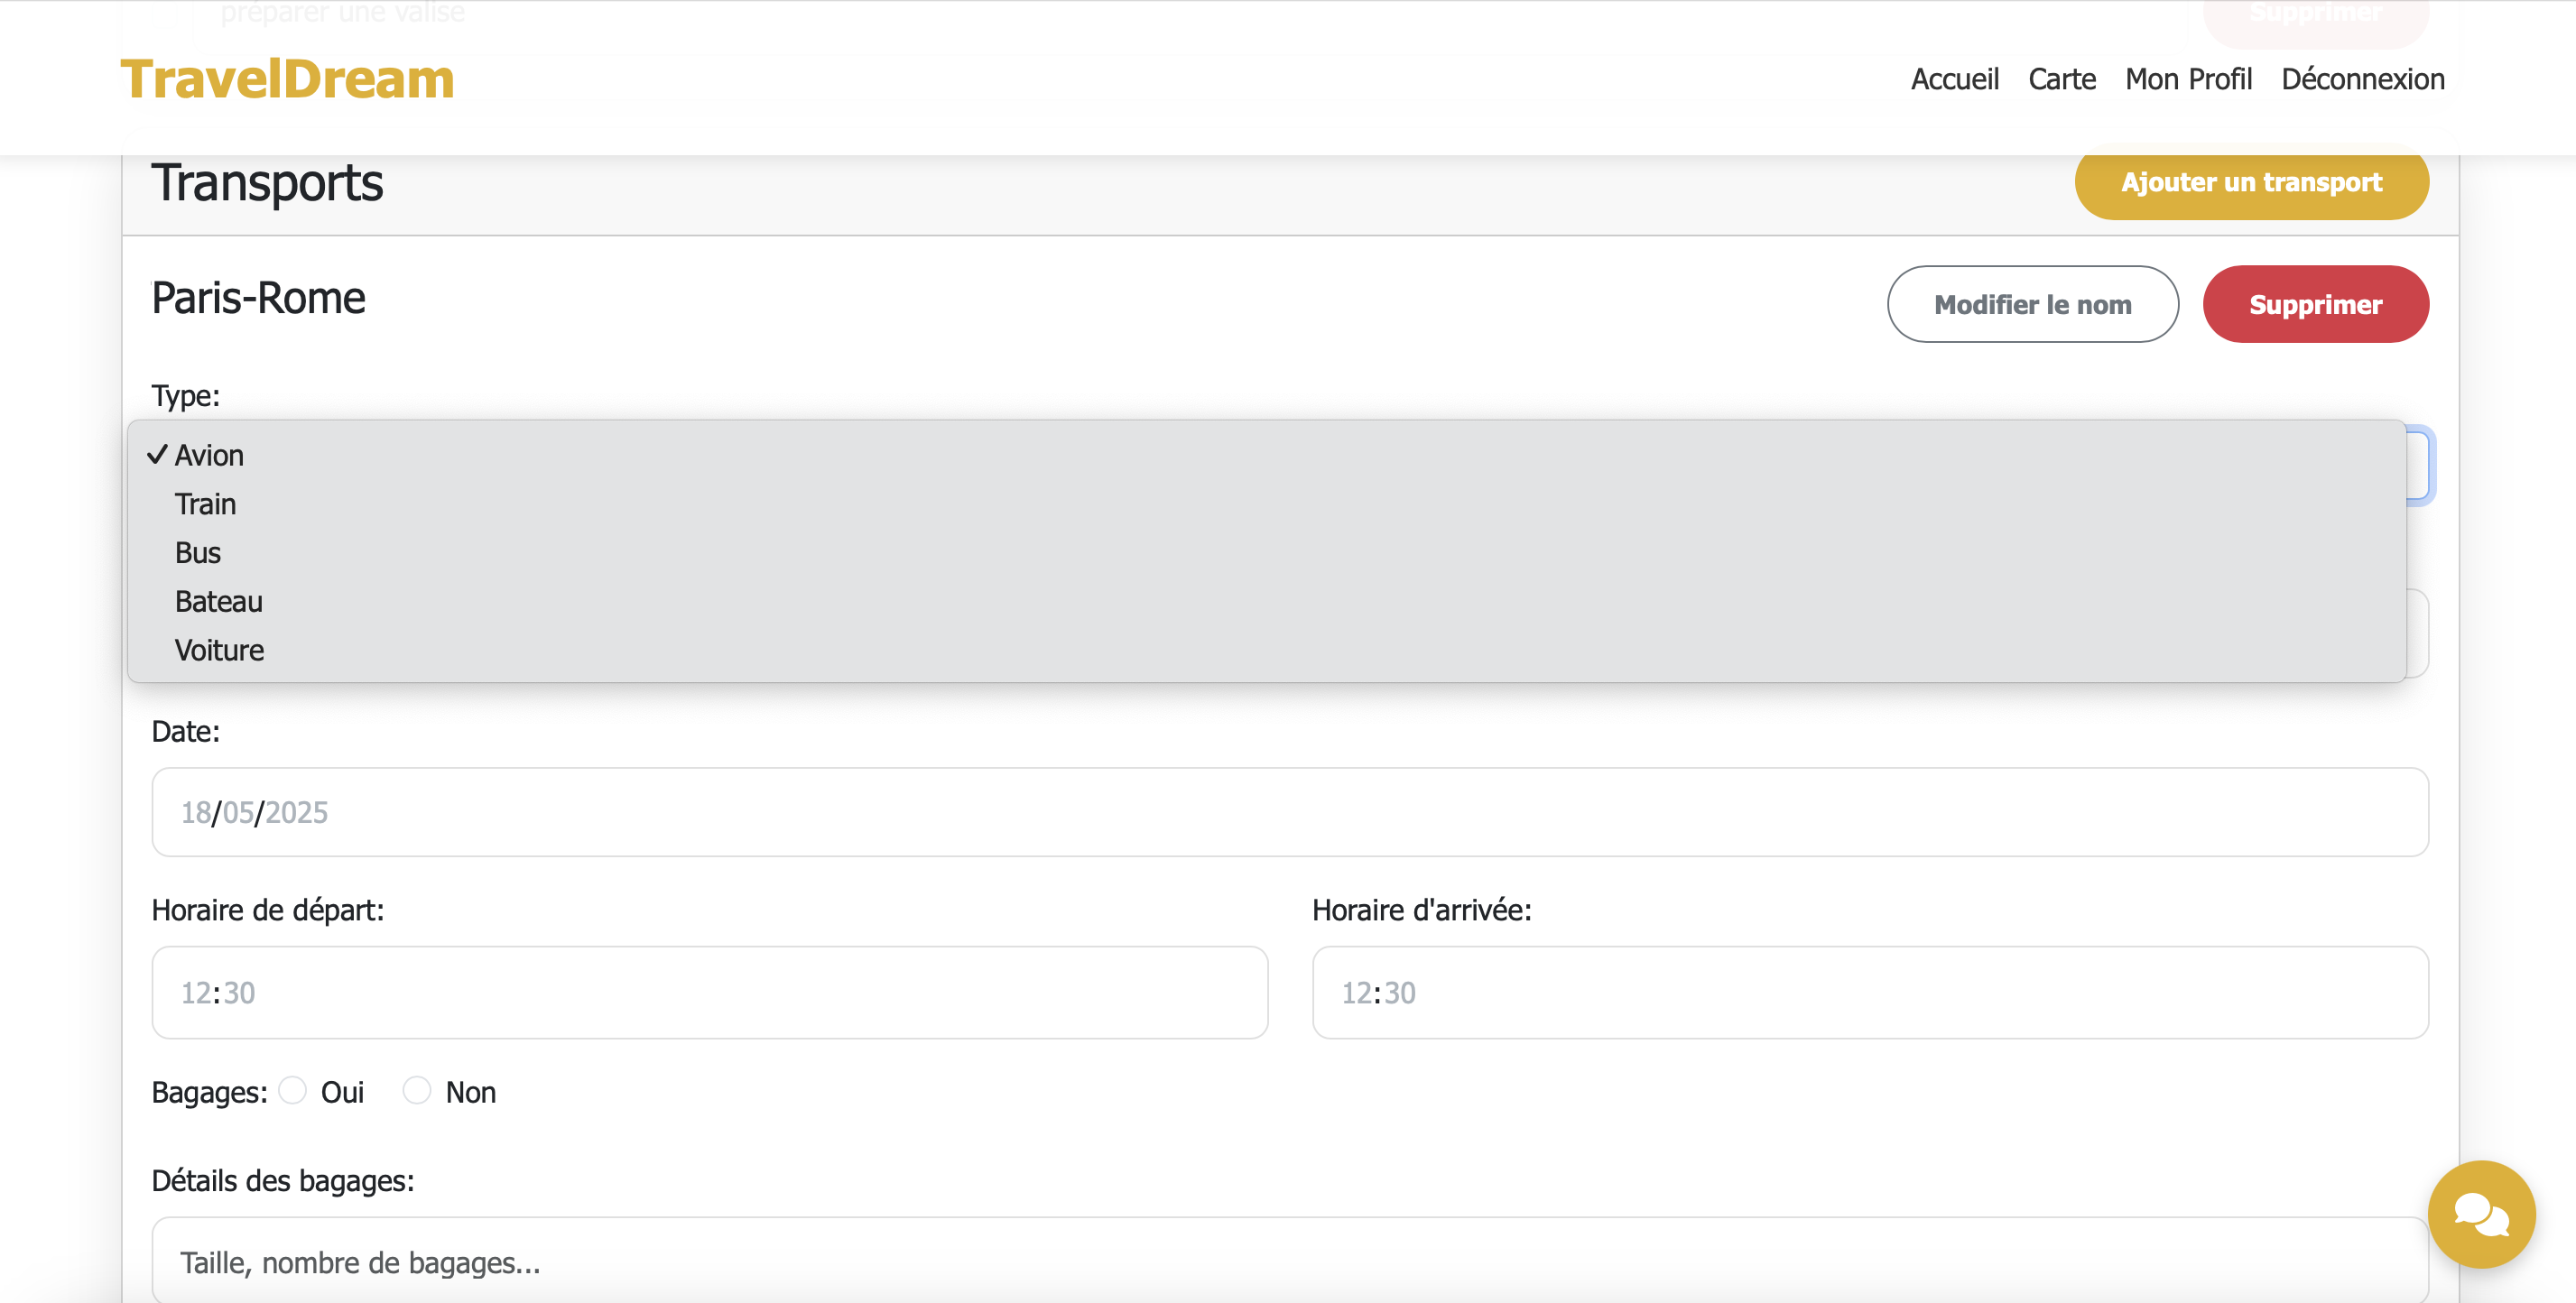
\includegraphics[width=0.8\textwidth]{8_creation_voyage_3_1.png}
\end{figure}
\begin{figure}[H]
    \centering
    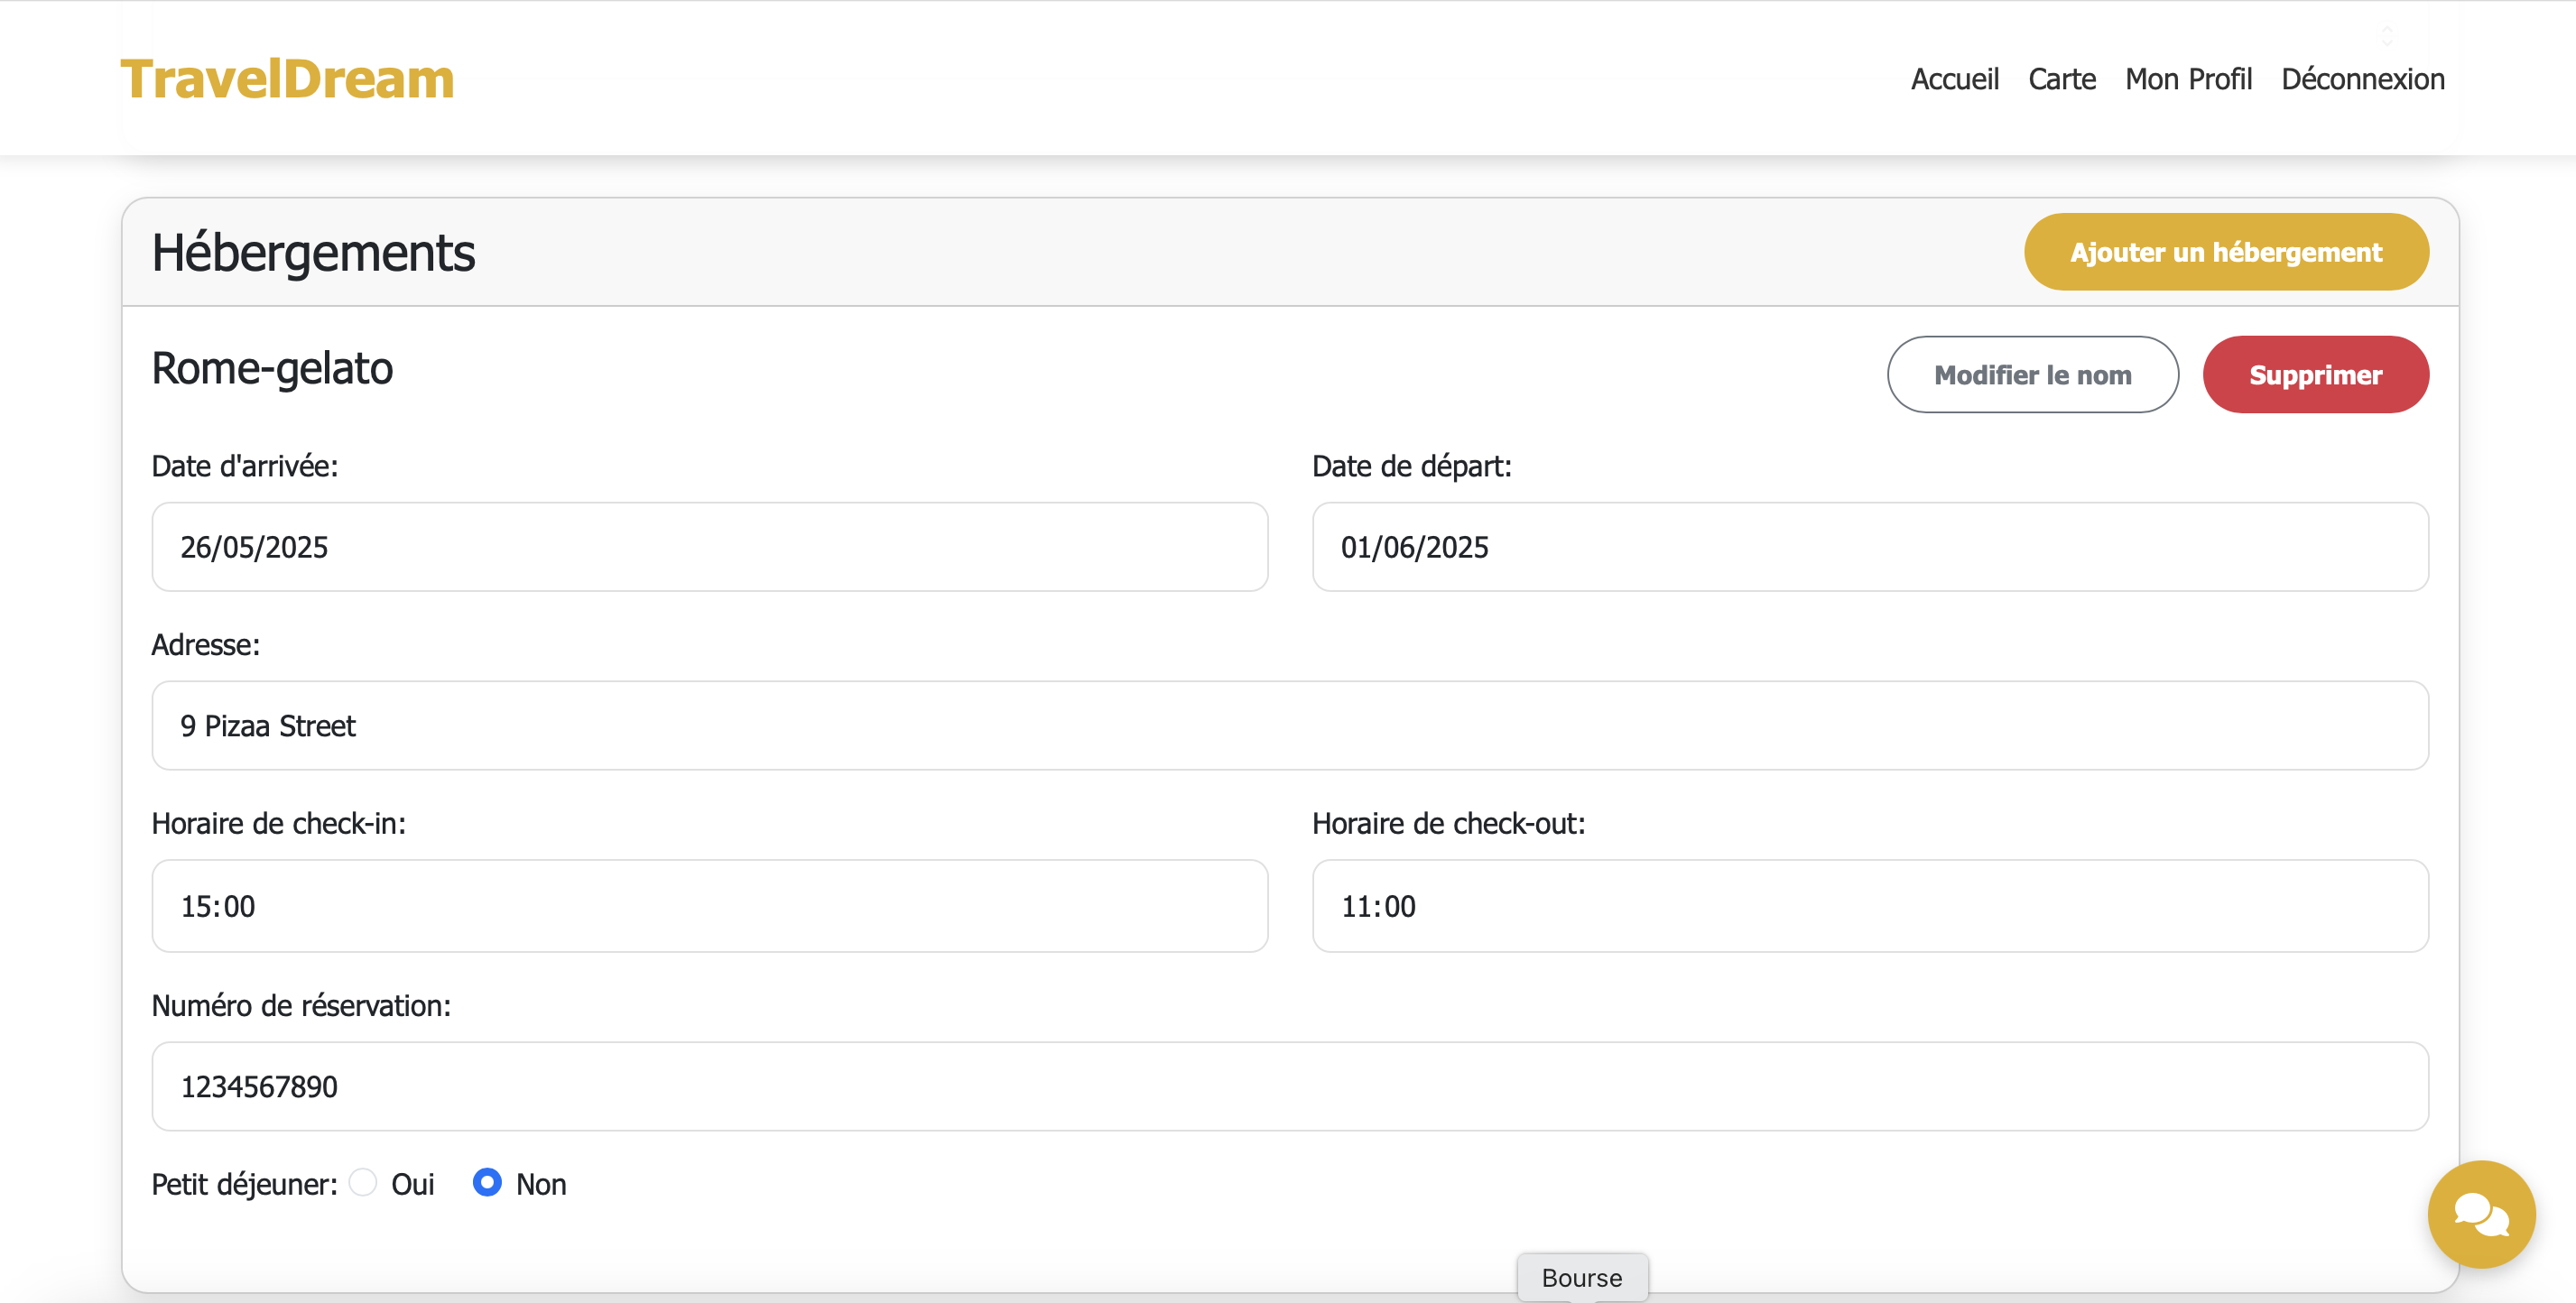
\includegraphics[width=0.8\textwidth]{8_creation_voyage_4.png}
\end{figure}
\begin{figure}[H]
    \centering
    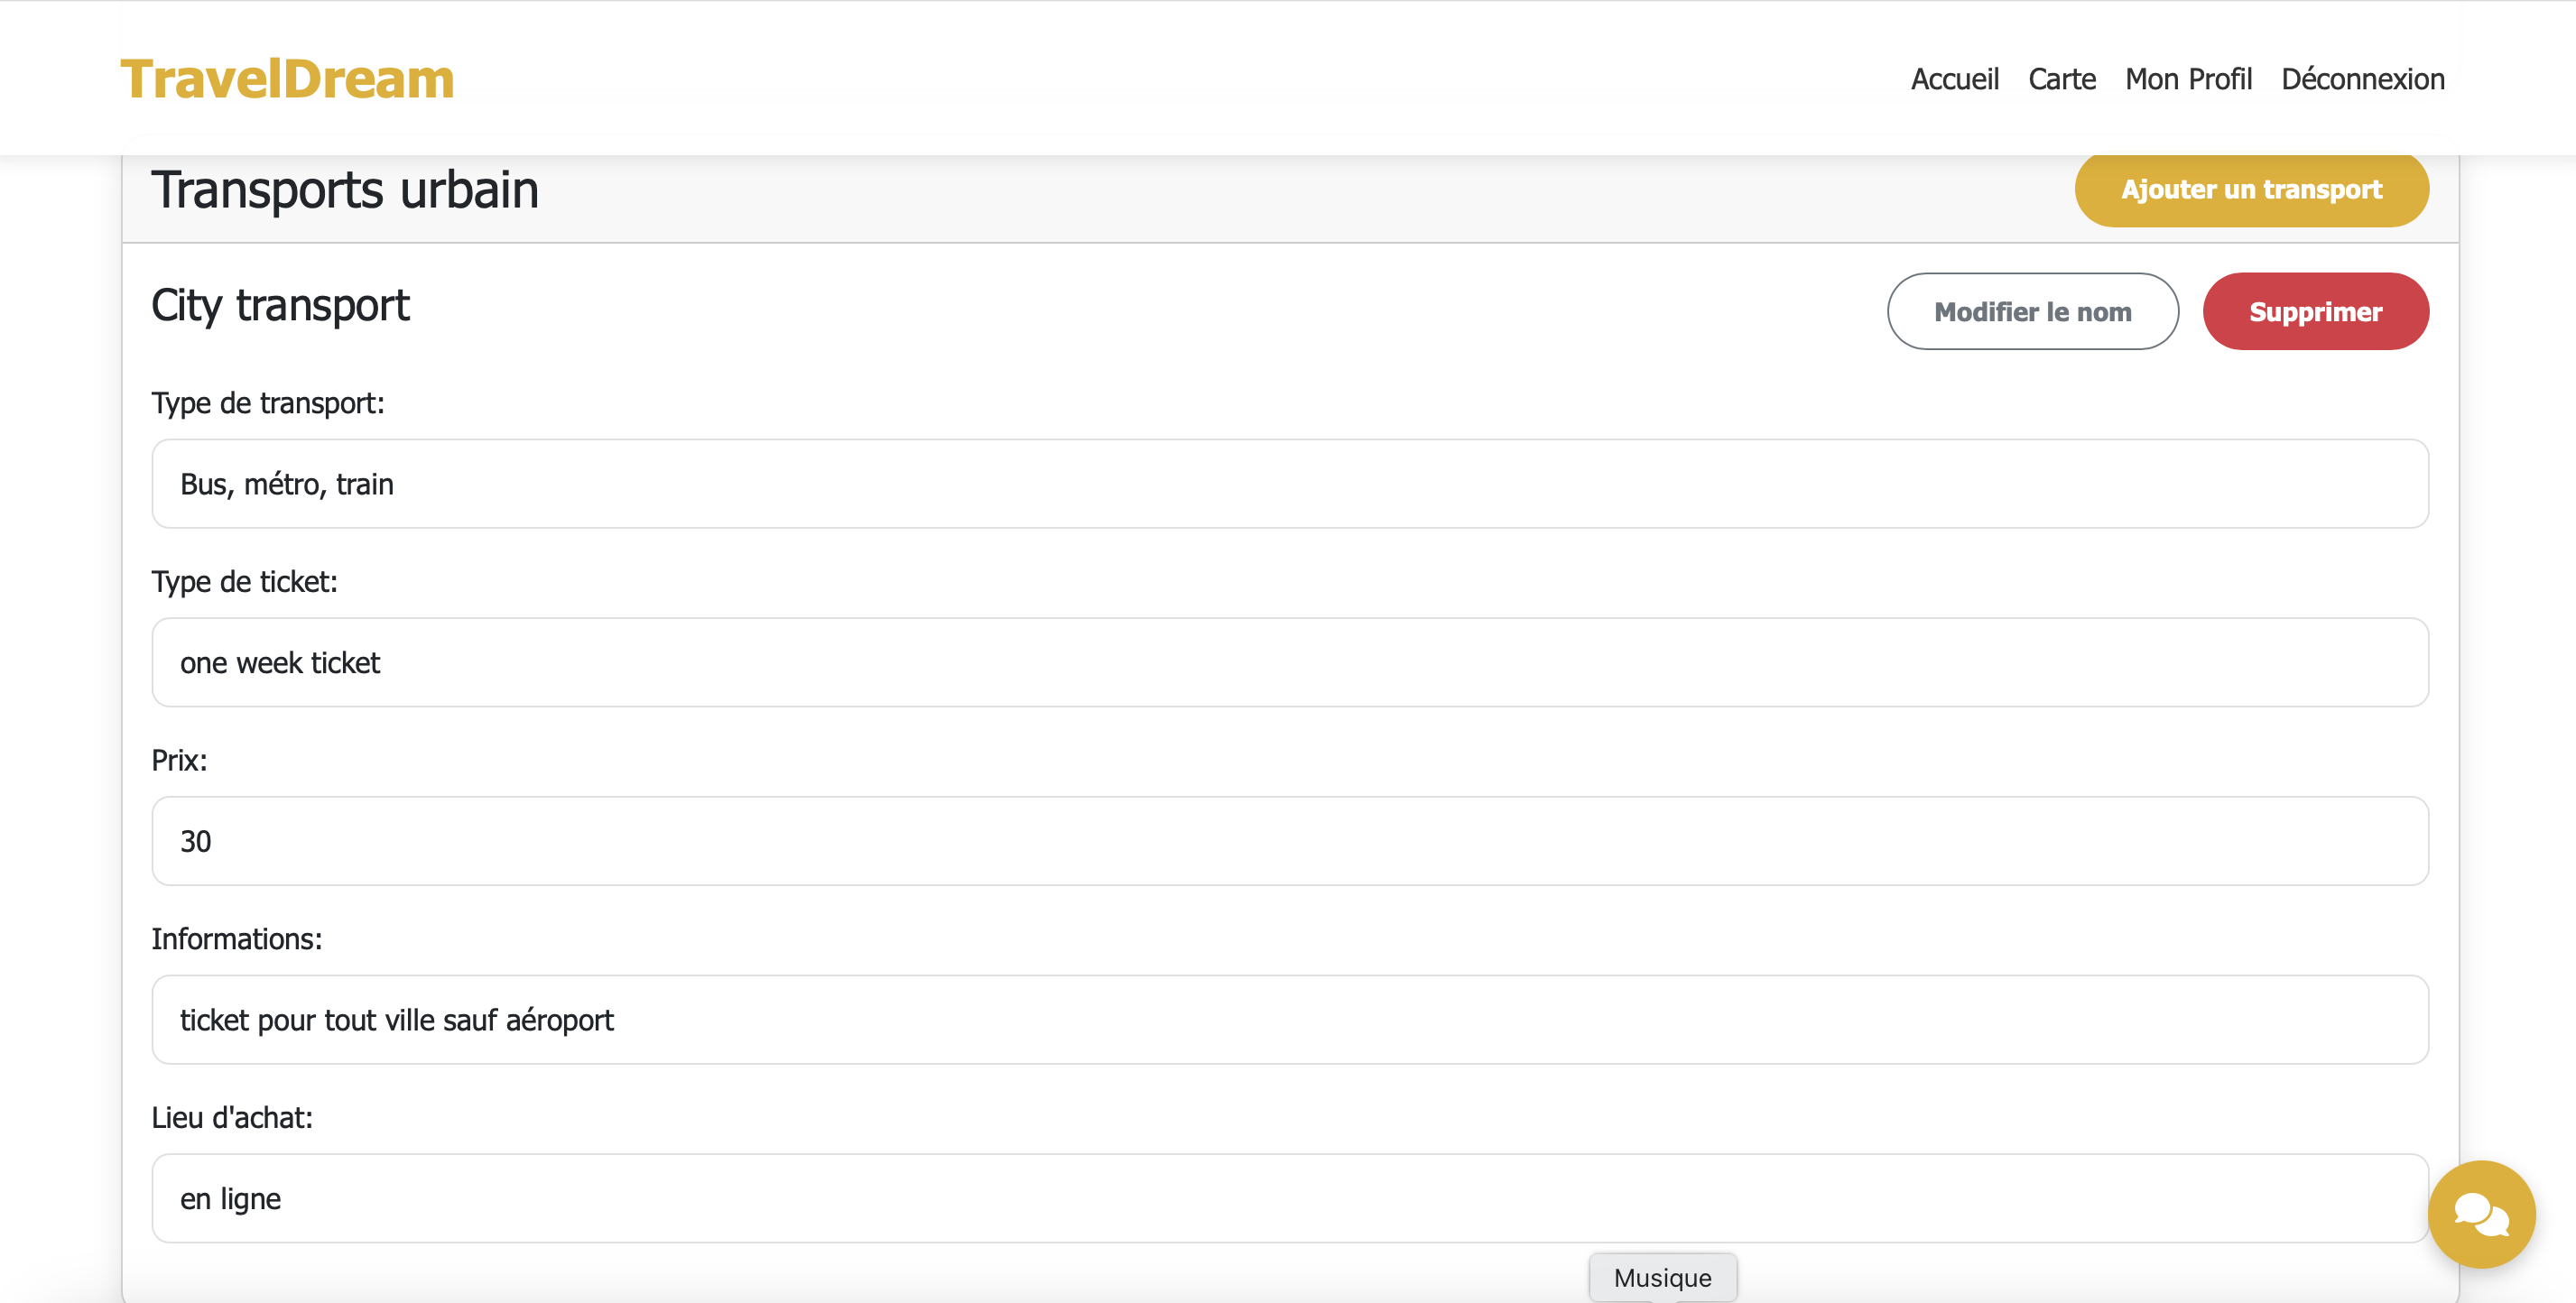
\includegraphics[width=0.8\textwidth]{8_creation_voyage_5.png}
\end{figure}
\begin{figure}[H]
    \centering
    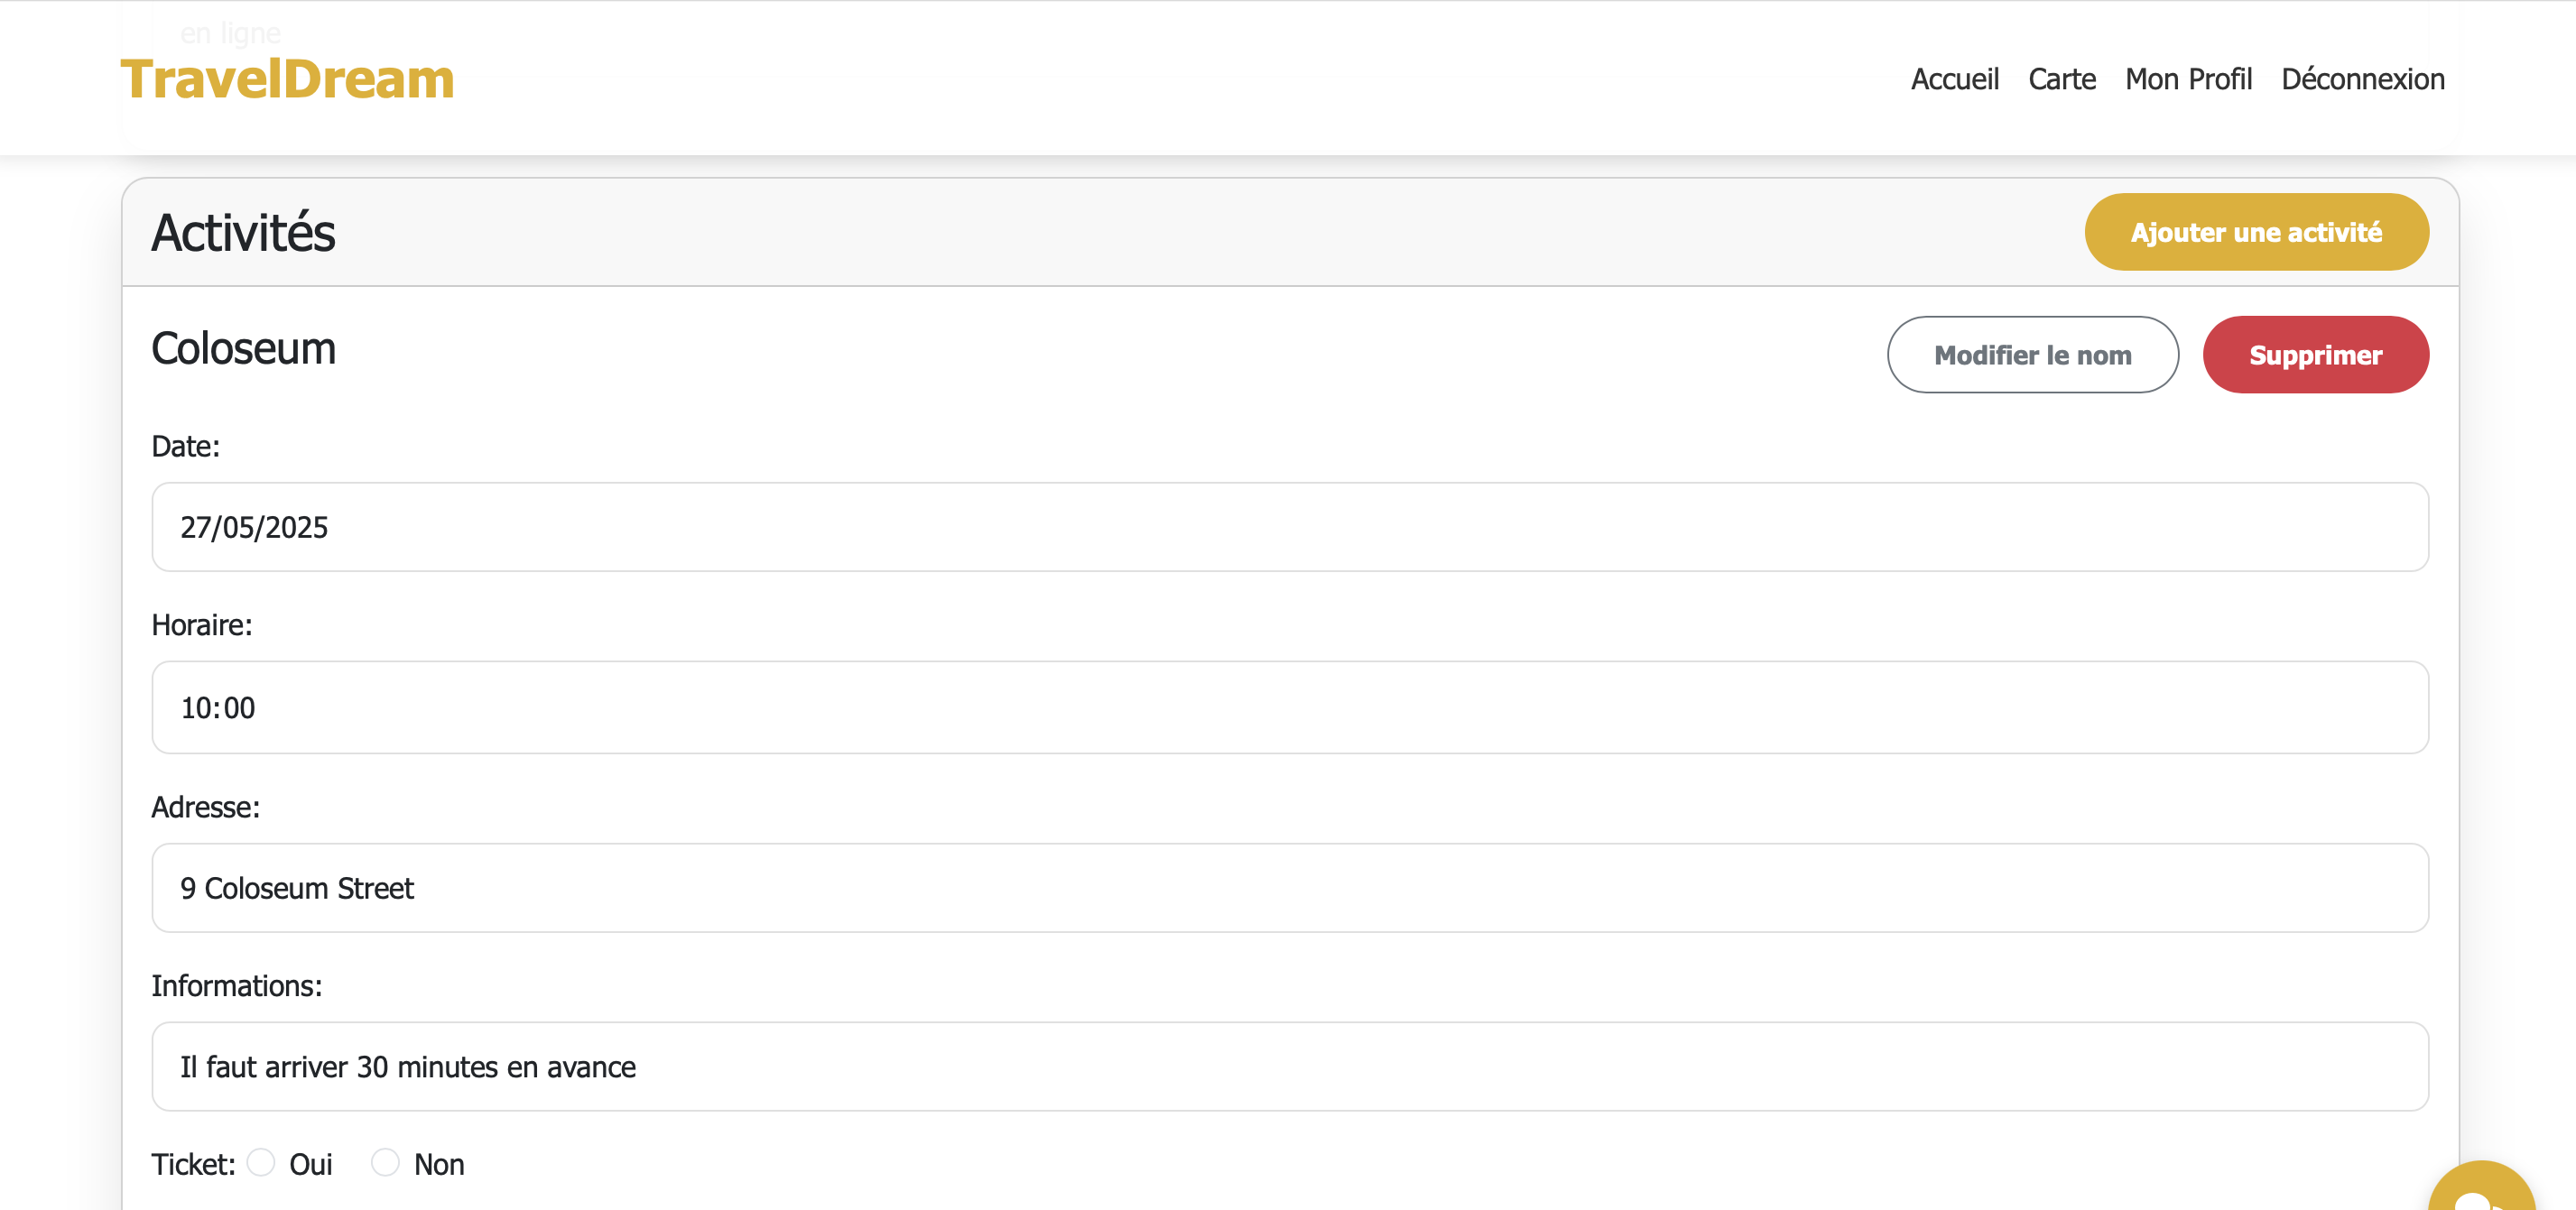
\includegraphics[width=0.8\textwidth]{8_creation_voyage_6.png}
\end{figure}
\begin{figure}[H]
    \centering
    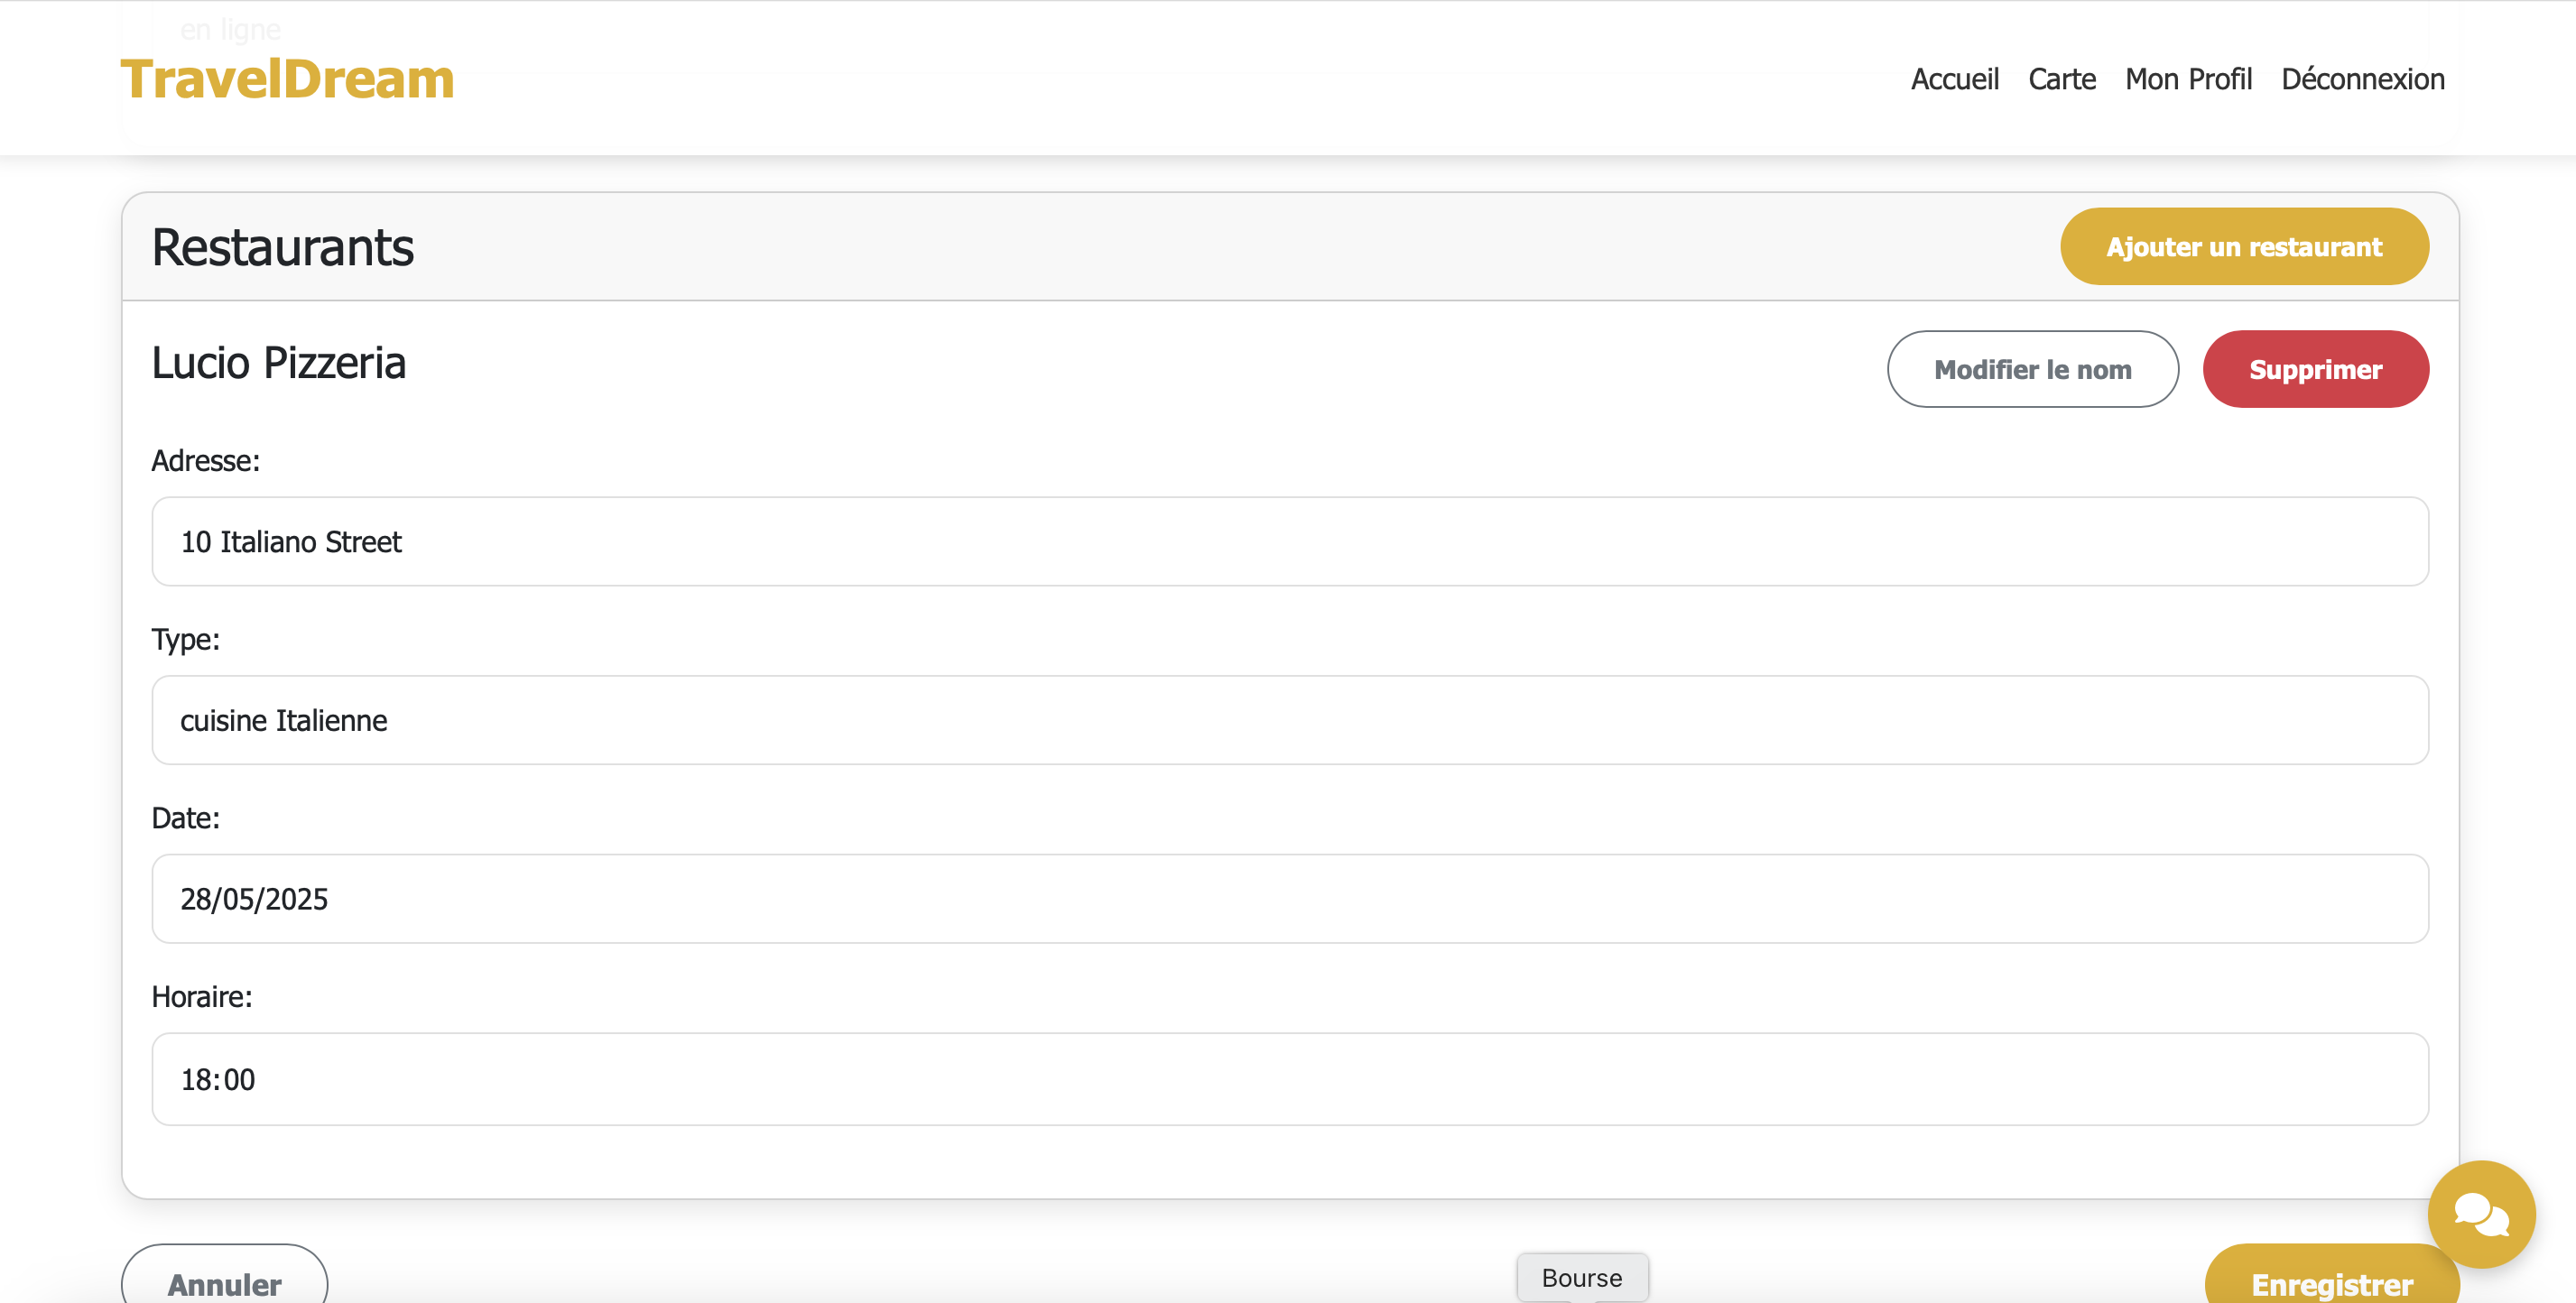
\includegraphics[width=0.8\textwidth]{8_creation_voyage_7.png}
\end{figure}


\subsubsection{Détail d'un voyage}
Accessible en cliquant sur "Détail" depuis "Mon profil" à partir d'un voyage déjà créé
\begin{figure}[H]
    \centering
    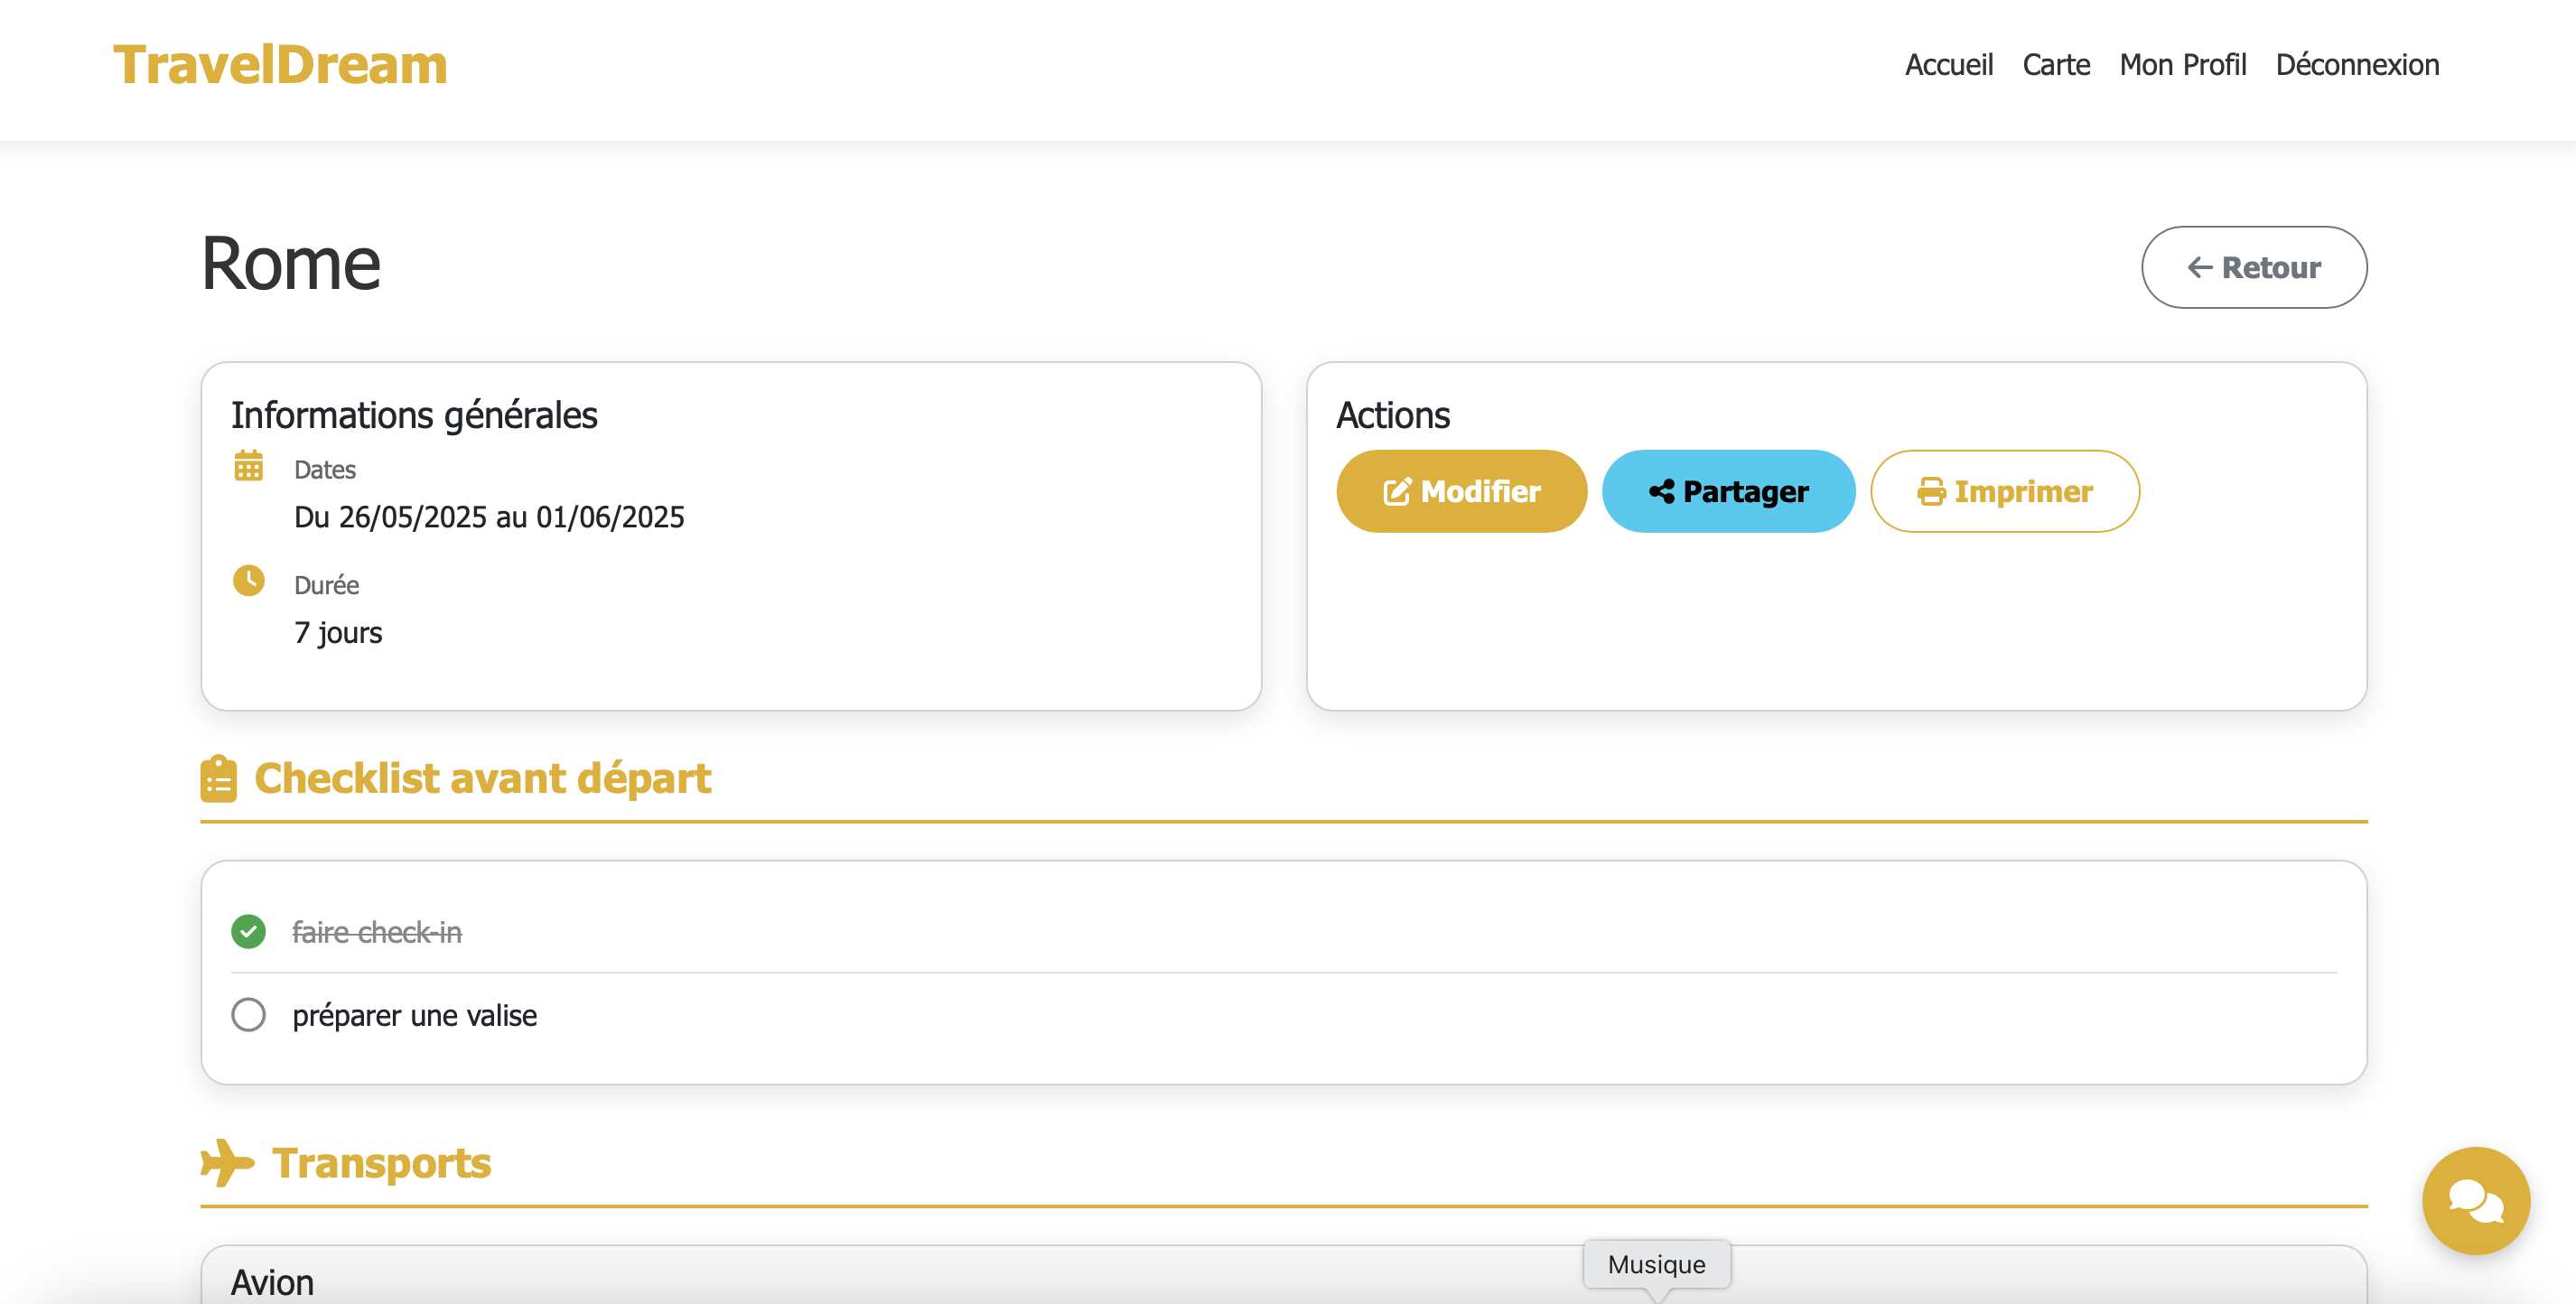
\includegraphics[width=0.8\textwidth]{9_detail_voyage_1.png}
\end{figure}
\begin{figure}[H]
    \centering
    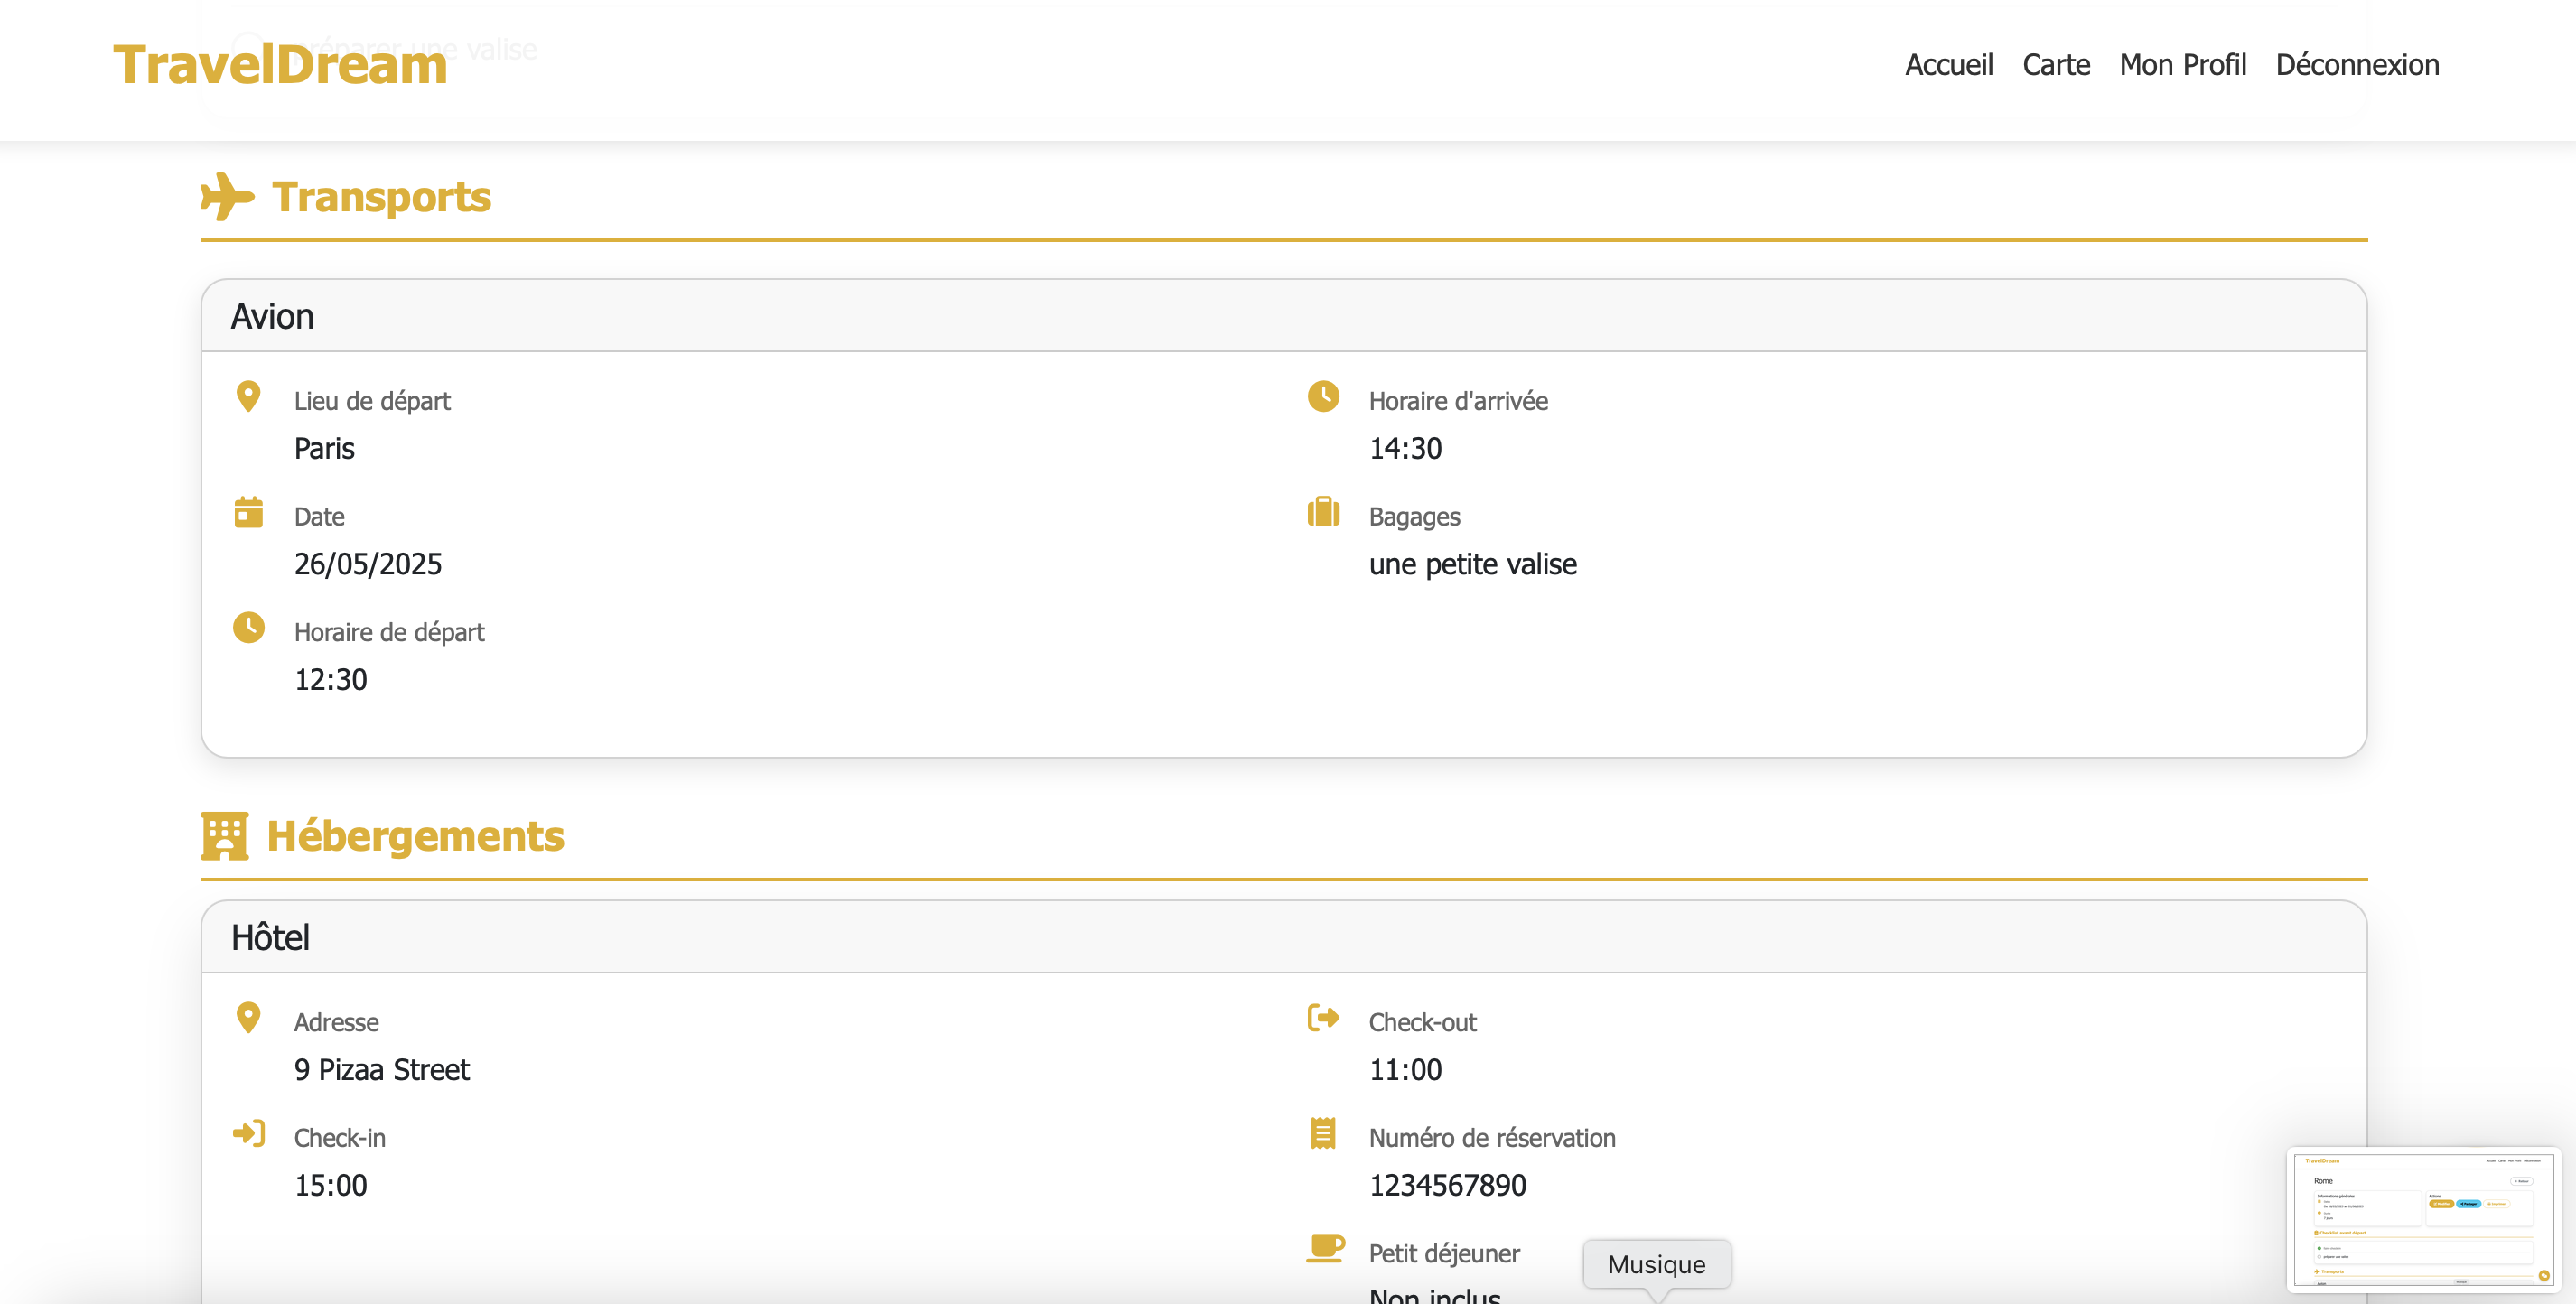
\includegraphics[width=0.8\textwidth]{9_detail_voyage_2.png}
\end{figure}
\begin{figure}[H]
    \centering
    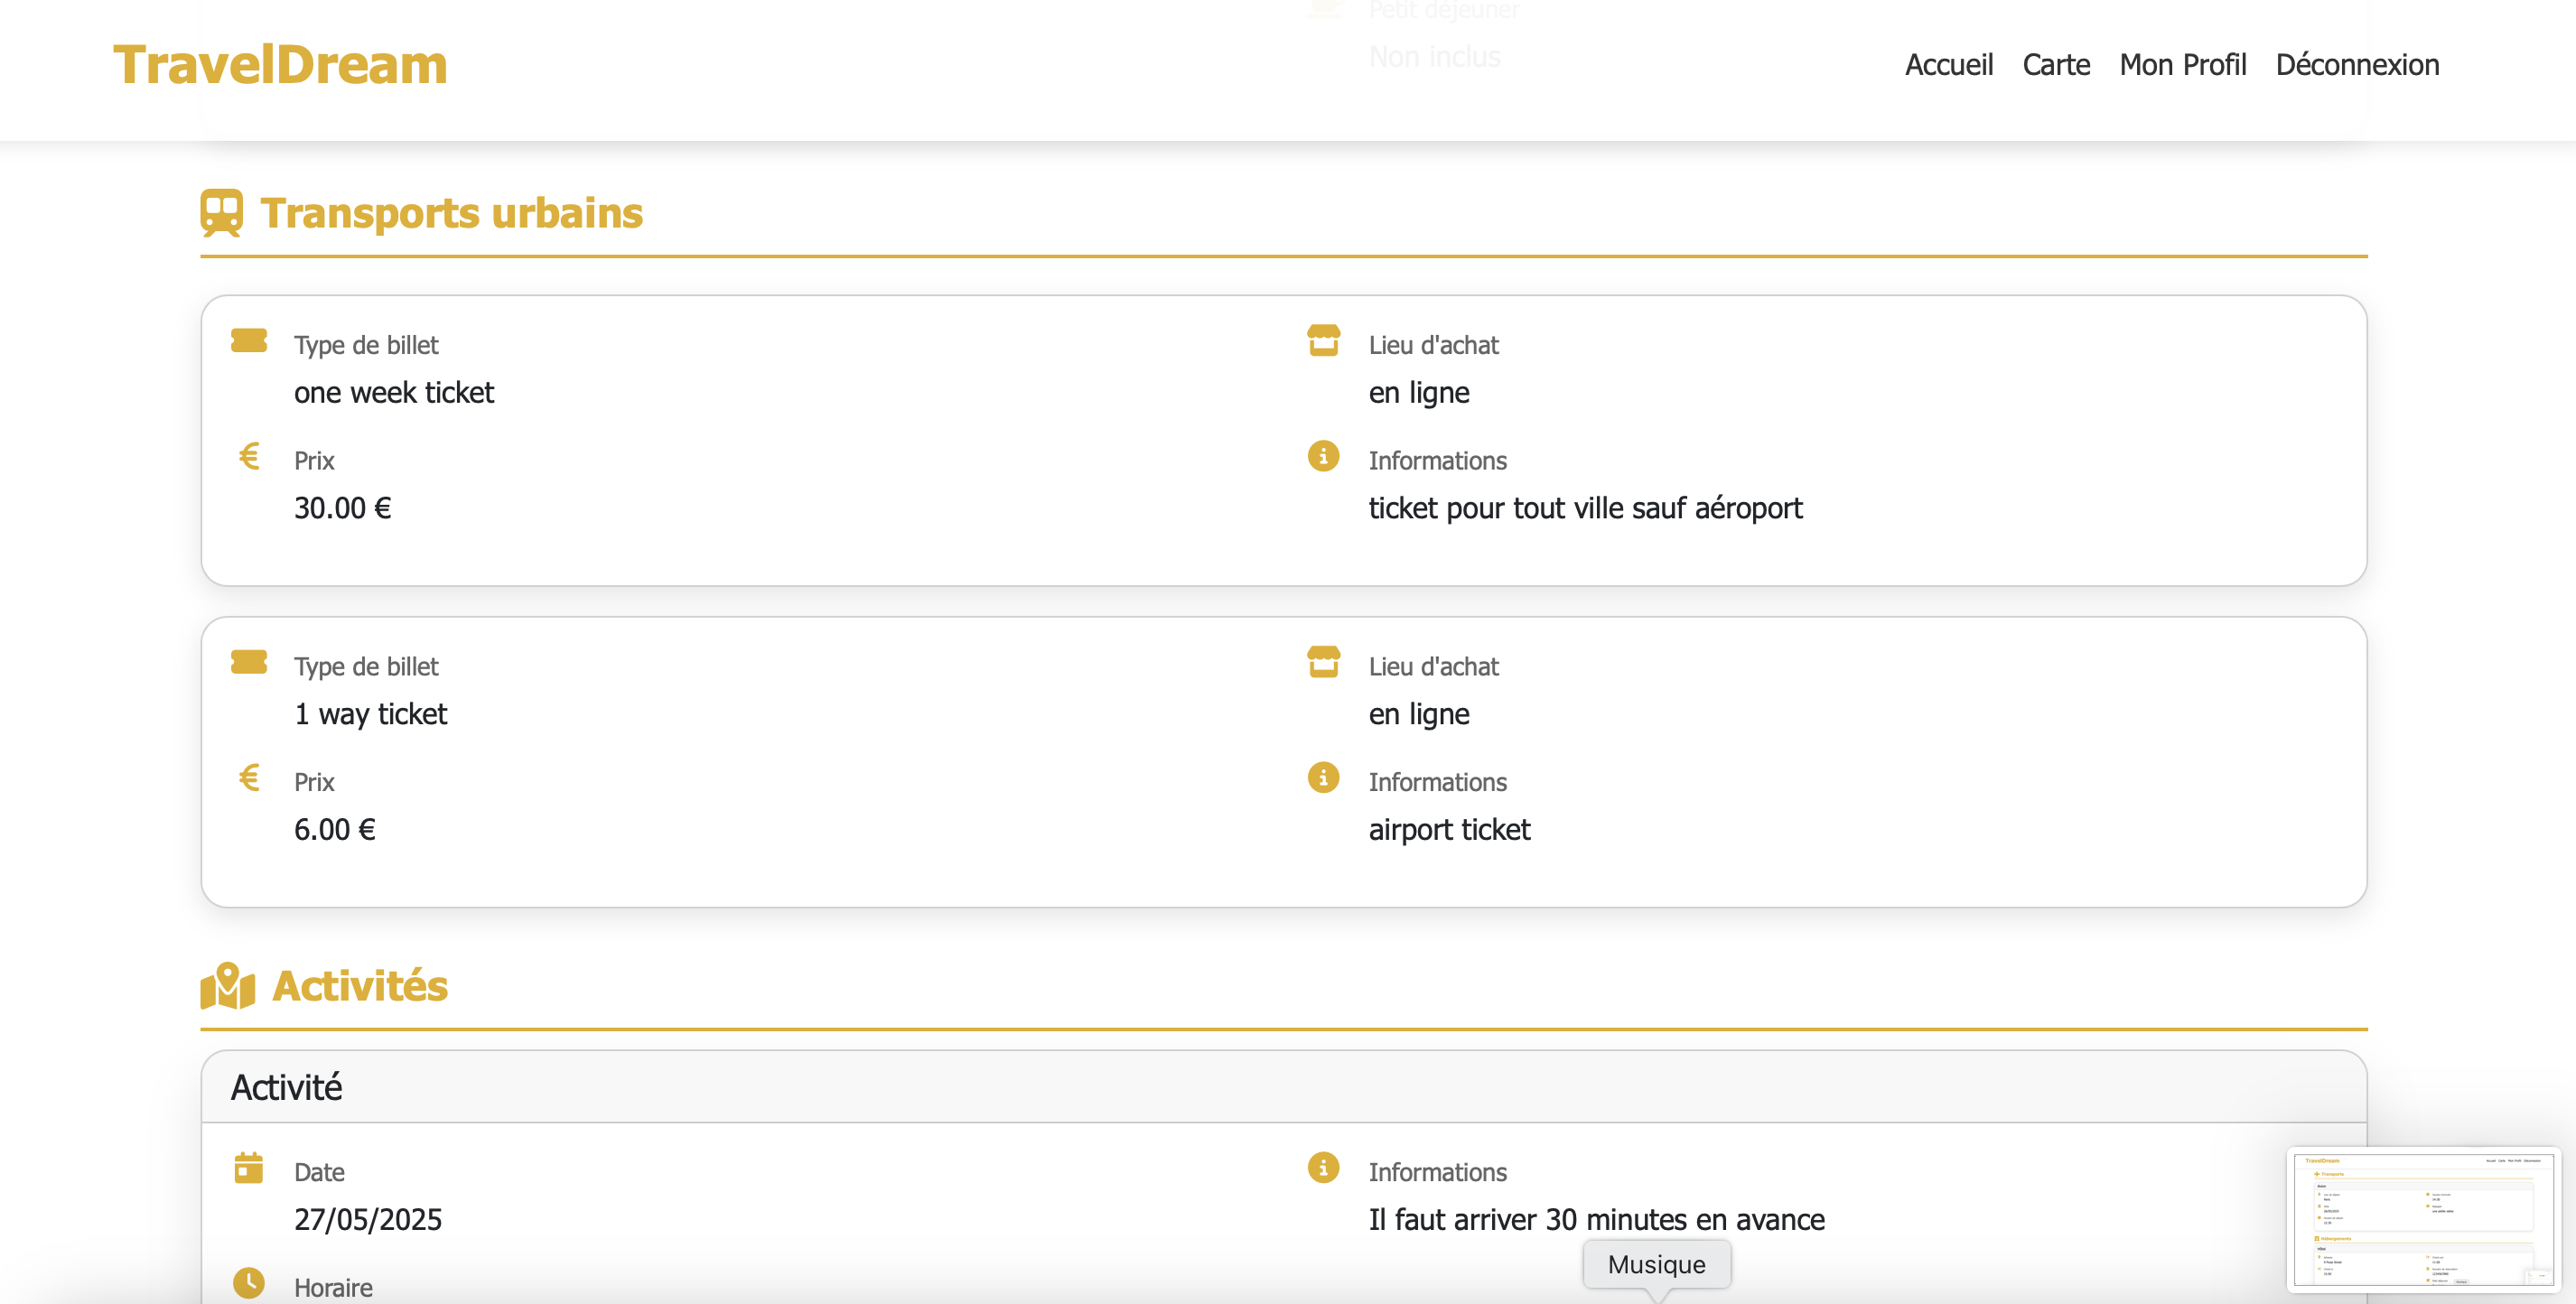
\includegraphics[width=0.8\textwidth]{9_detail_voyage_3.png}
\end{figure}
\begin{figure}[H]
    \centering
    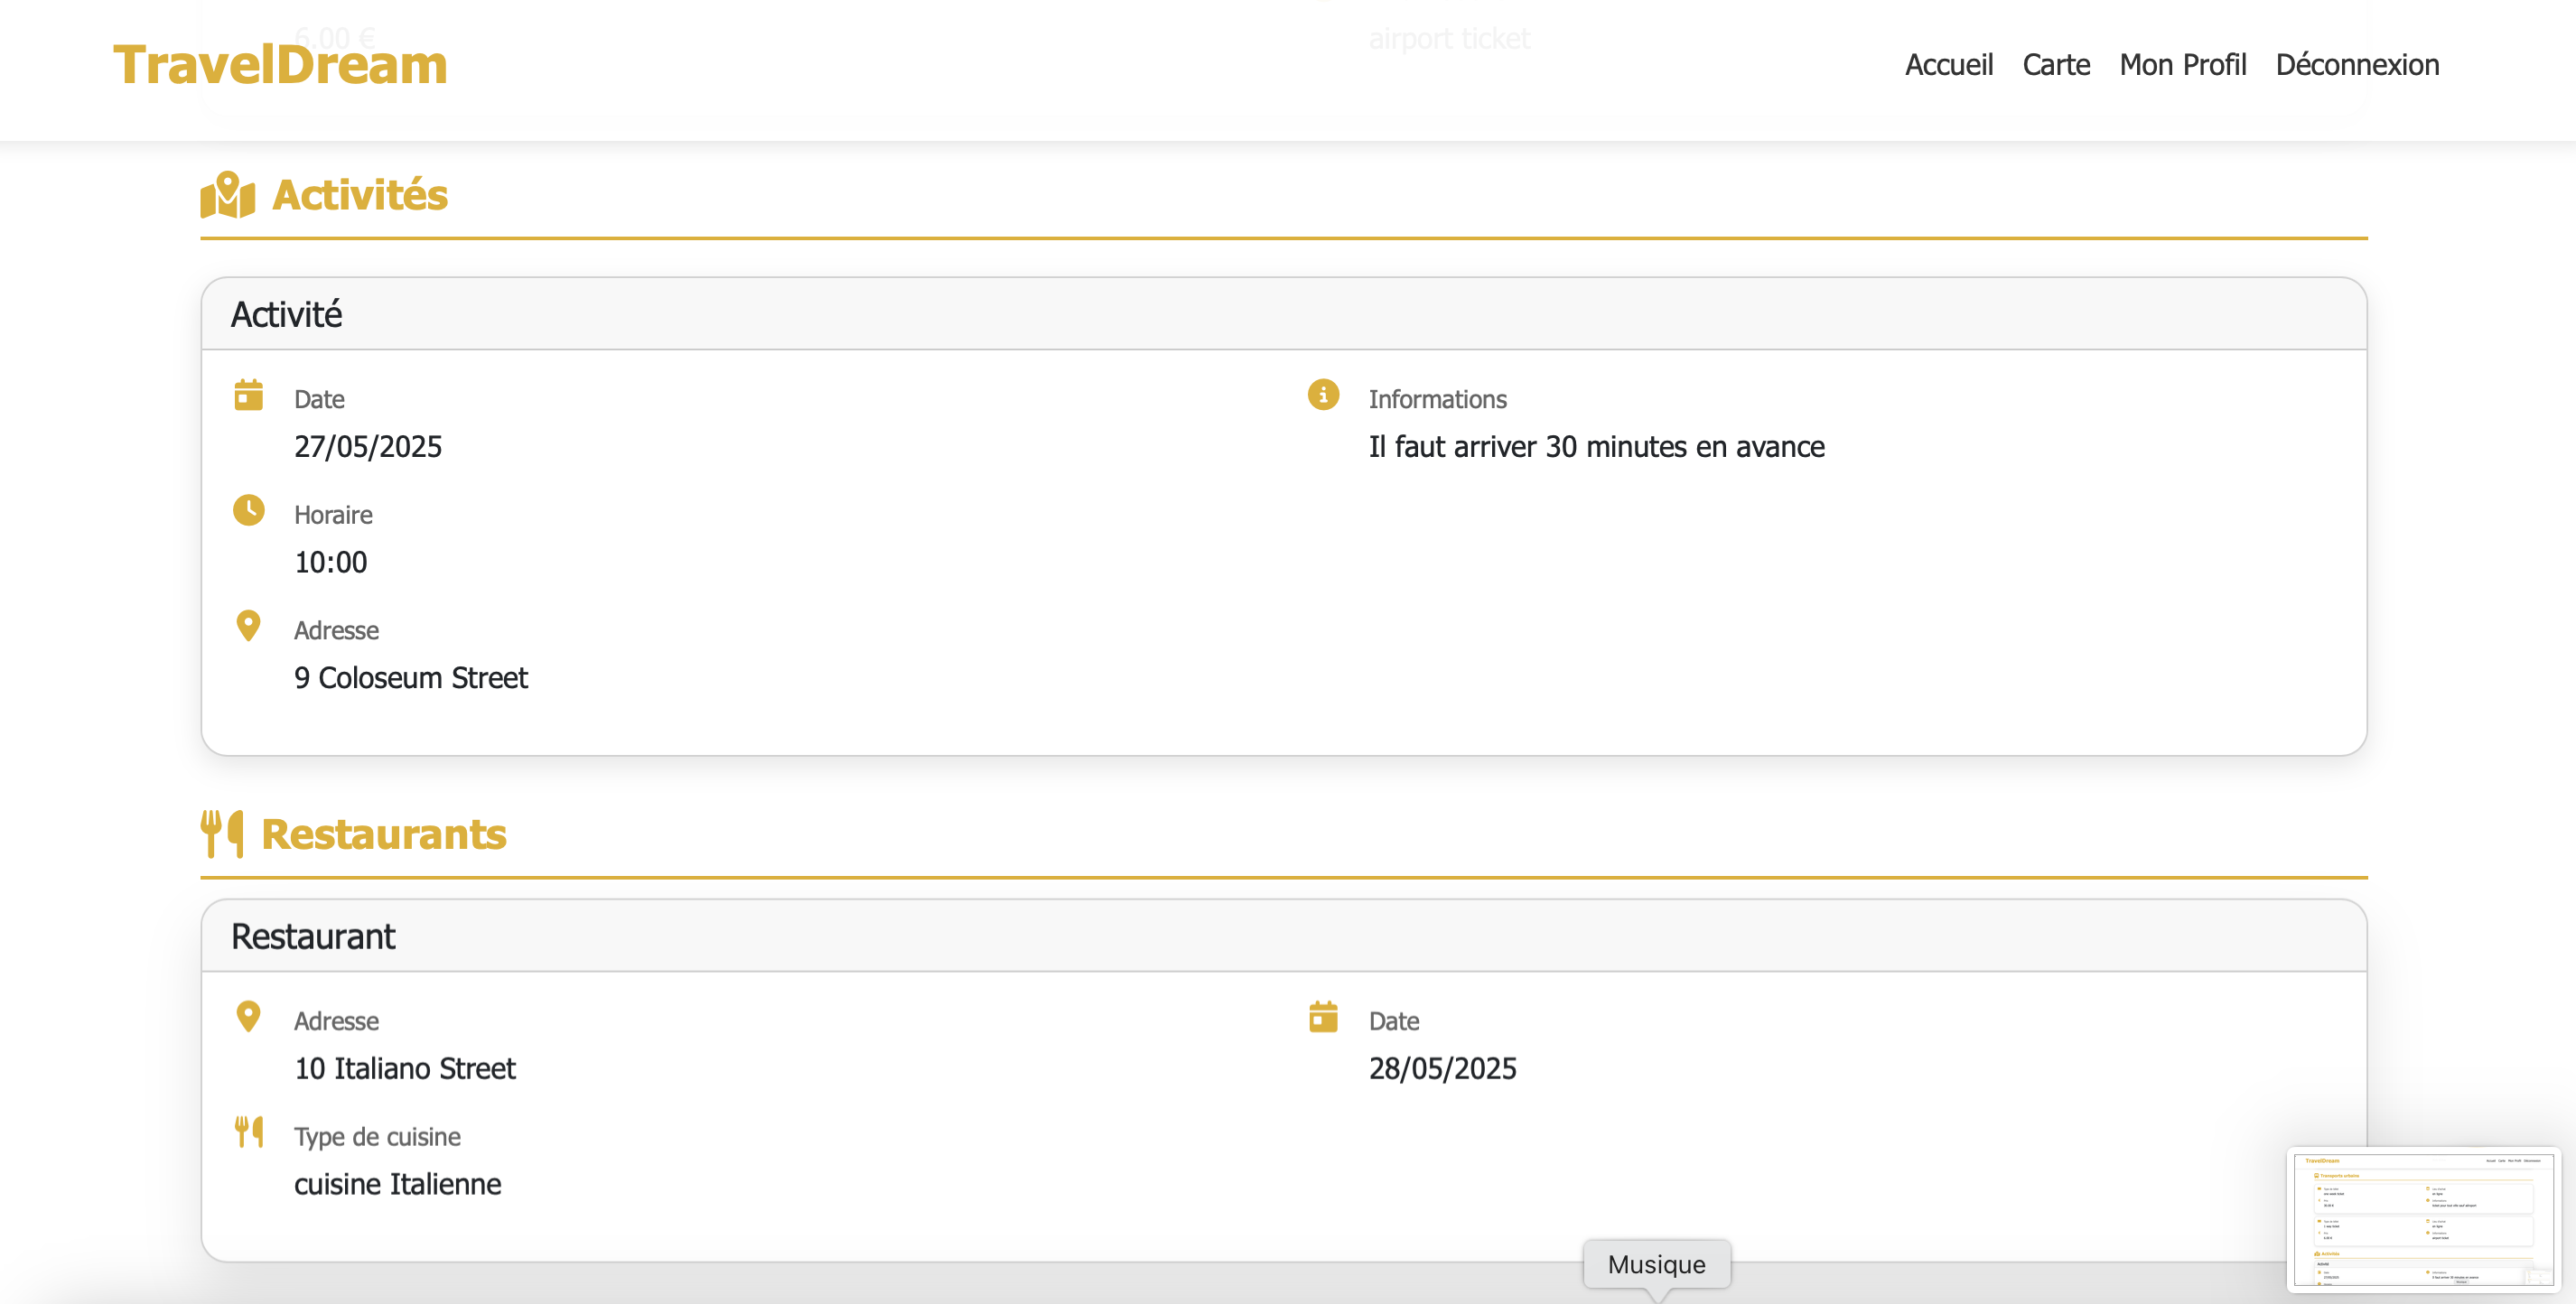
\includegraphics[width=0.8\textwidth]{9_detail_voyage_4.png}
\end{figure}


\subsubsection{Partager un voyage}
Accessible en cliquant sur "Partager" depuis "Mon profil" à partir d'un voyage déjà créé ou "Partager" à partir des détails du voyage
\begin{figure}[H]
    \centering
    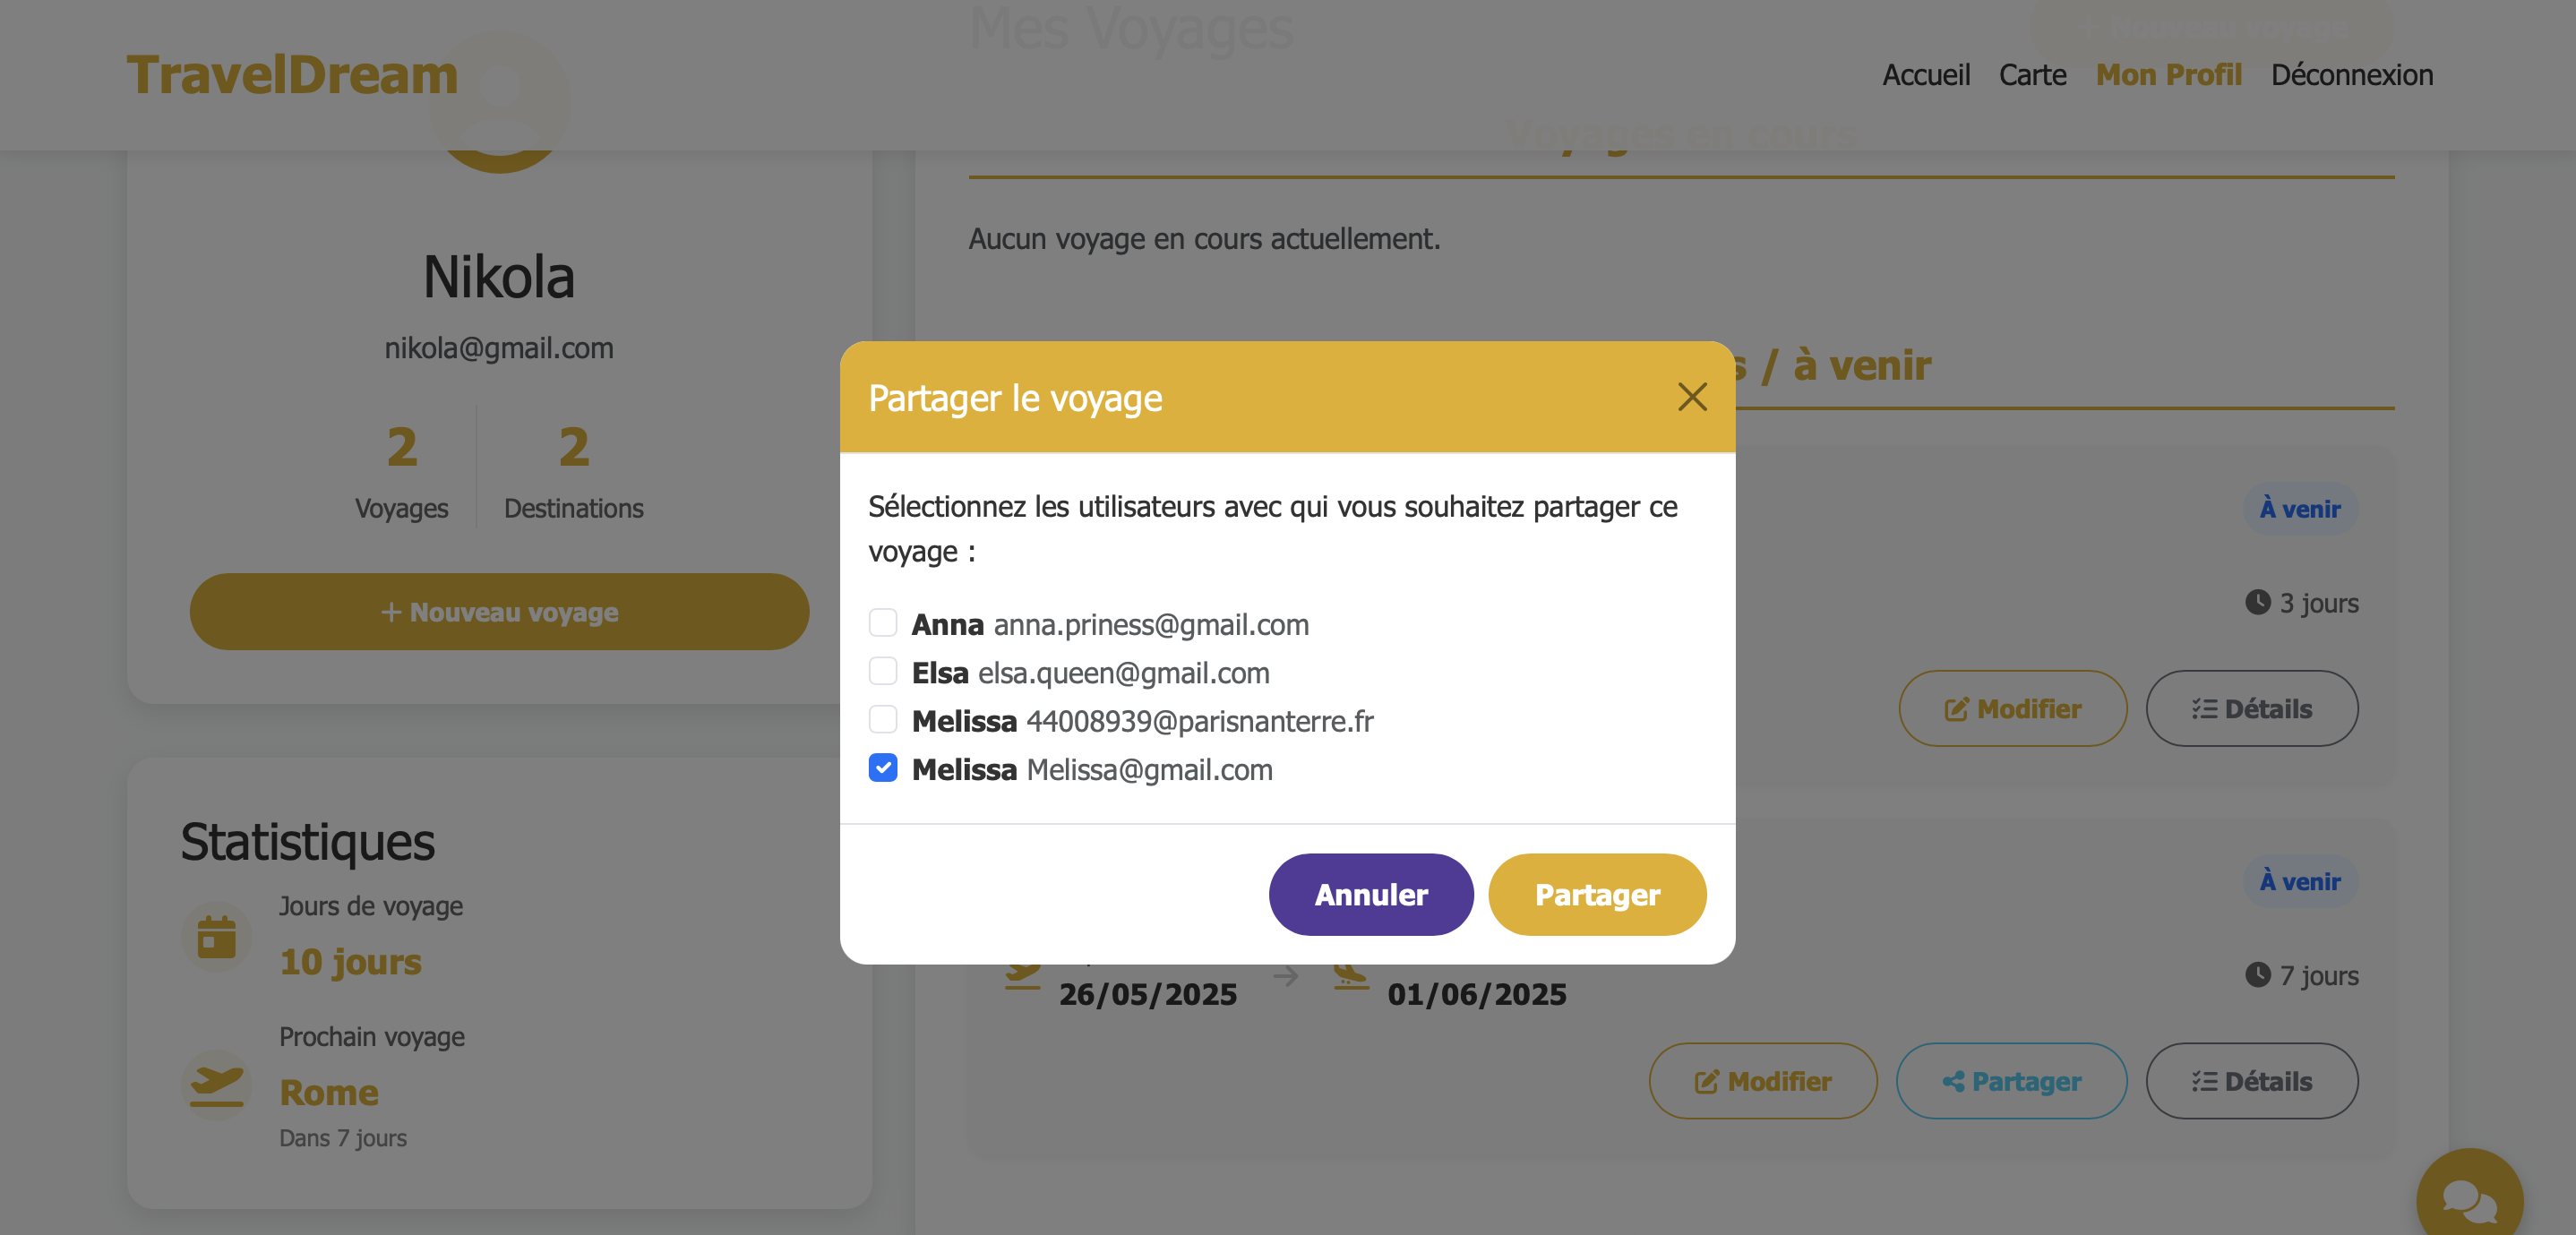
\includegraphics[width=0.8\textwidth]{10_partager_voyage_1.png}
\end{figure}
\begin{figure}[H]
    \centering
    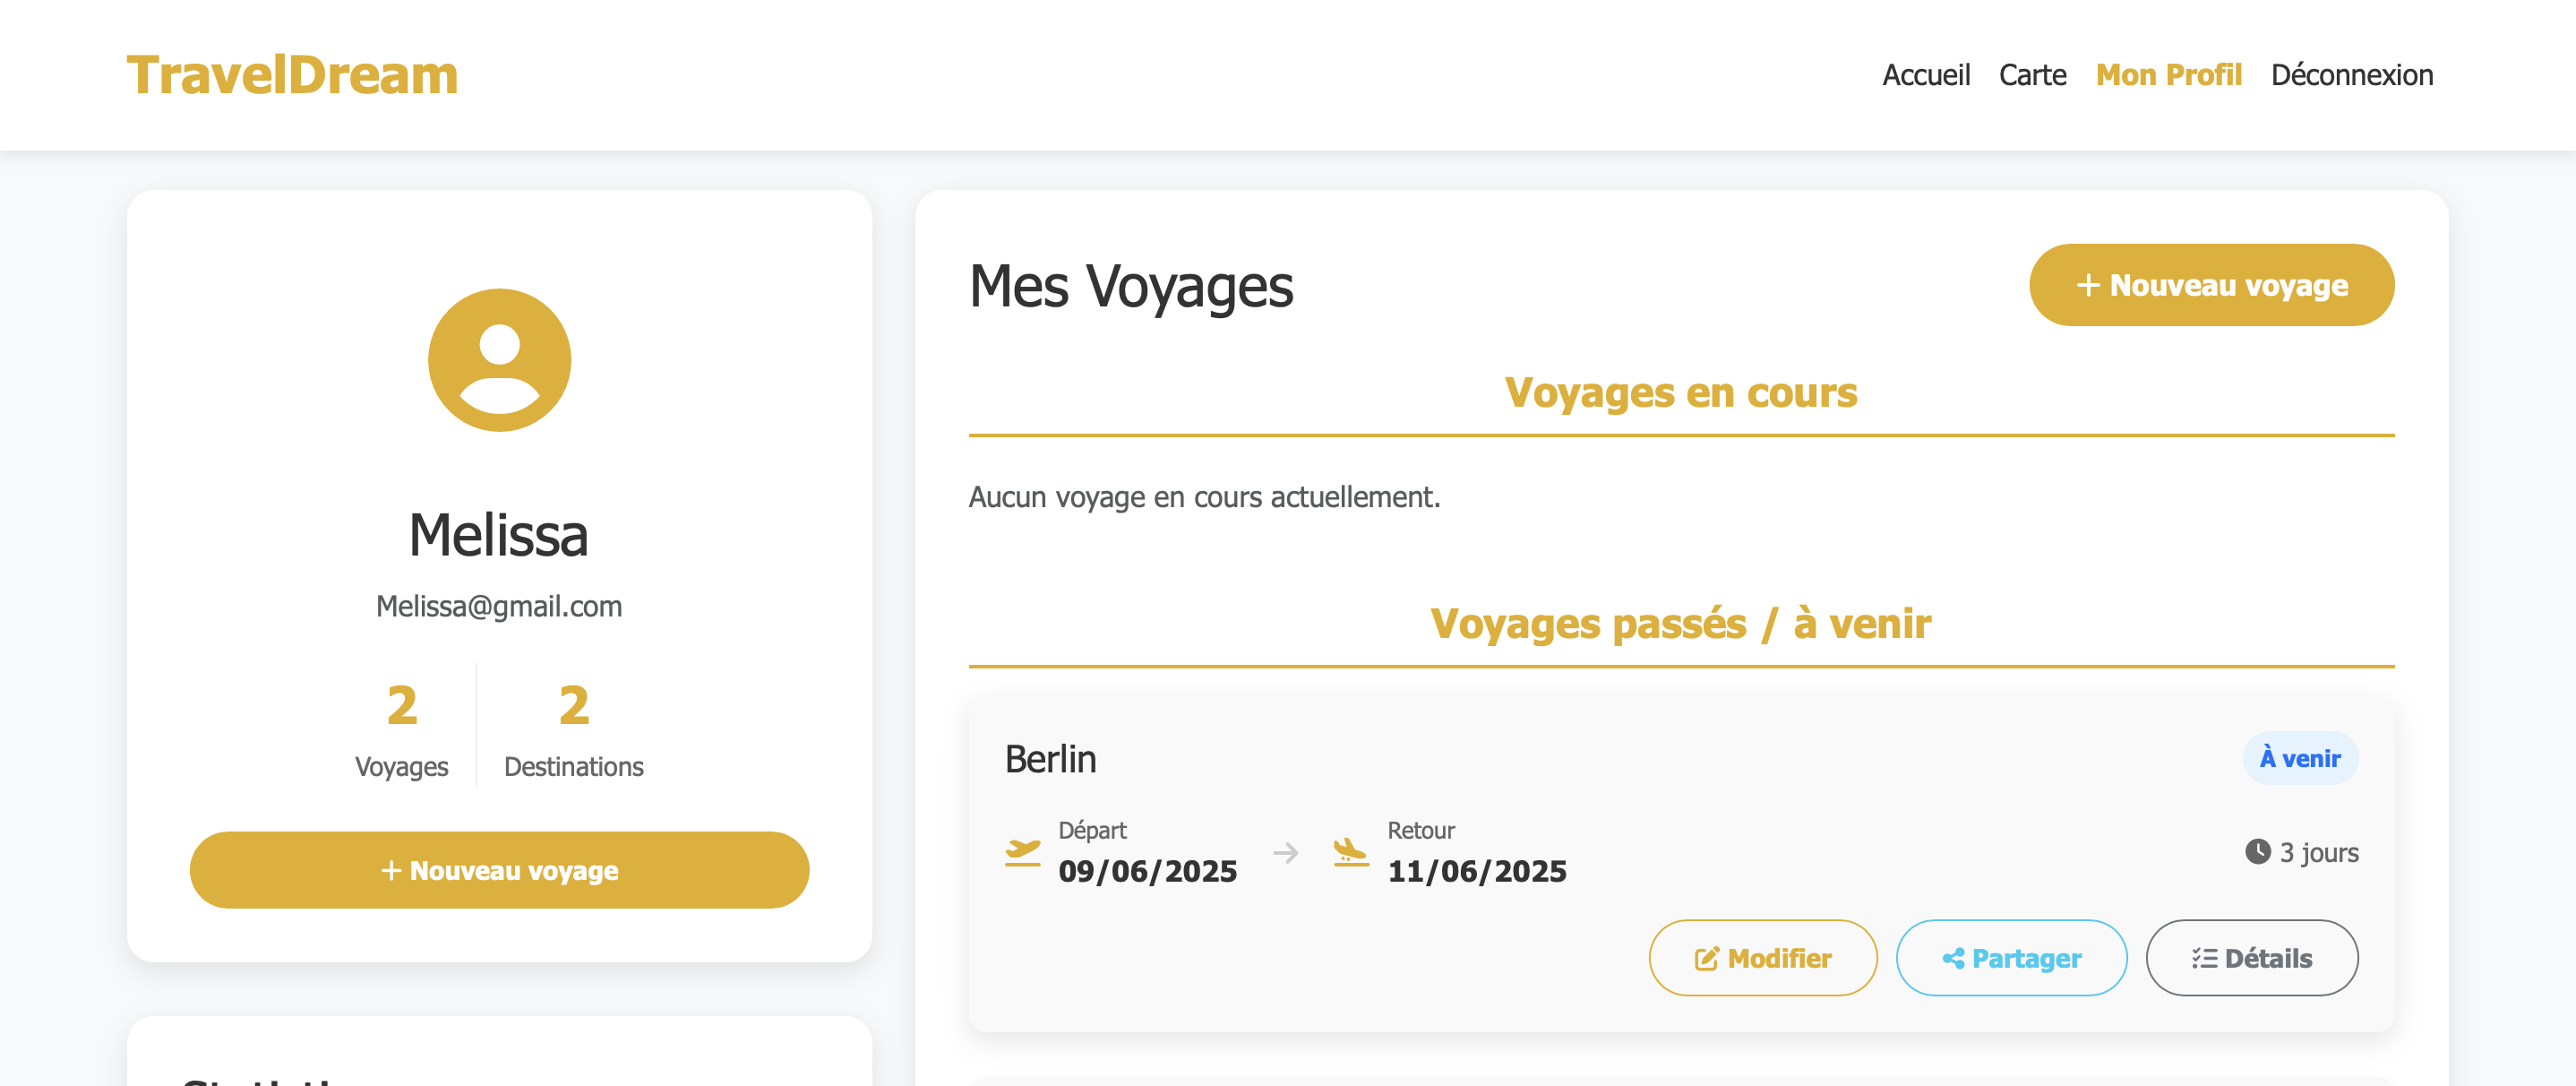
\includegraphics[width=0.8\textwidth]{10_partager_voyage_2.png}
\end{figure}

\subsubsection{Imprimer un voyage}
Accessible en cliquant "Imprimer" à partir des détails du voyage
\begin{figure}[H]
    \centering
    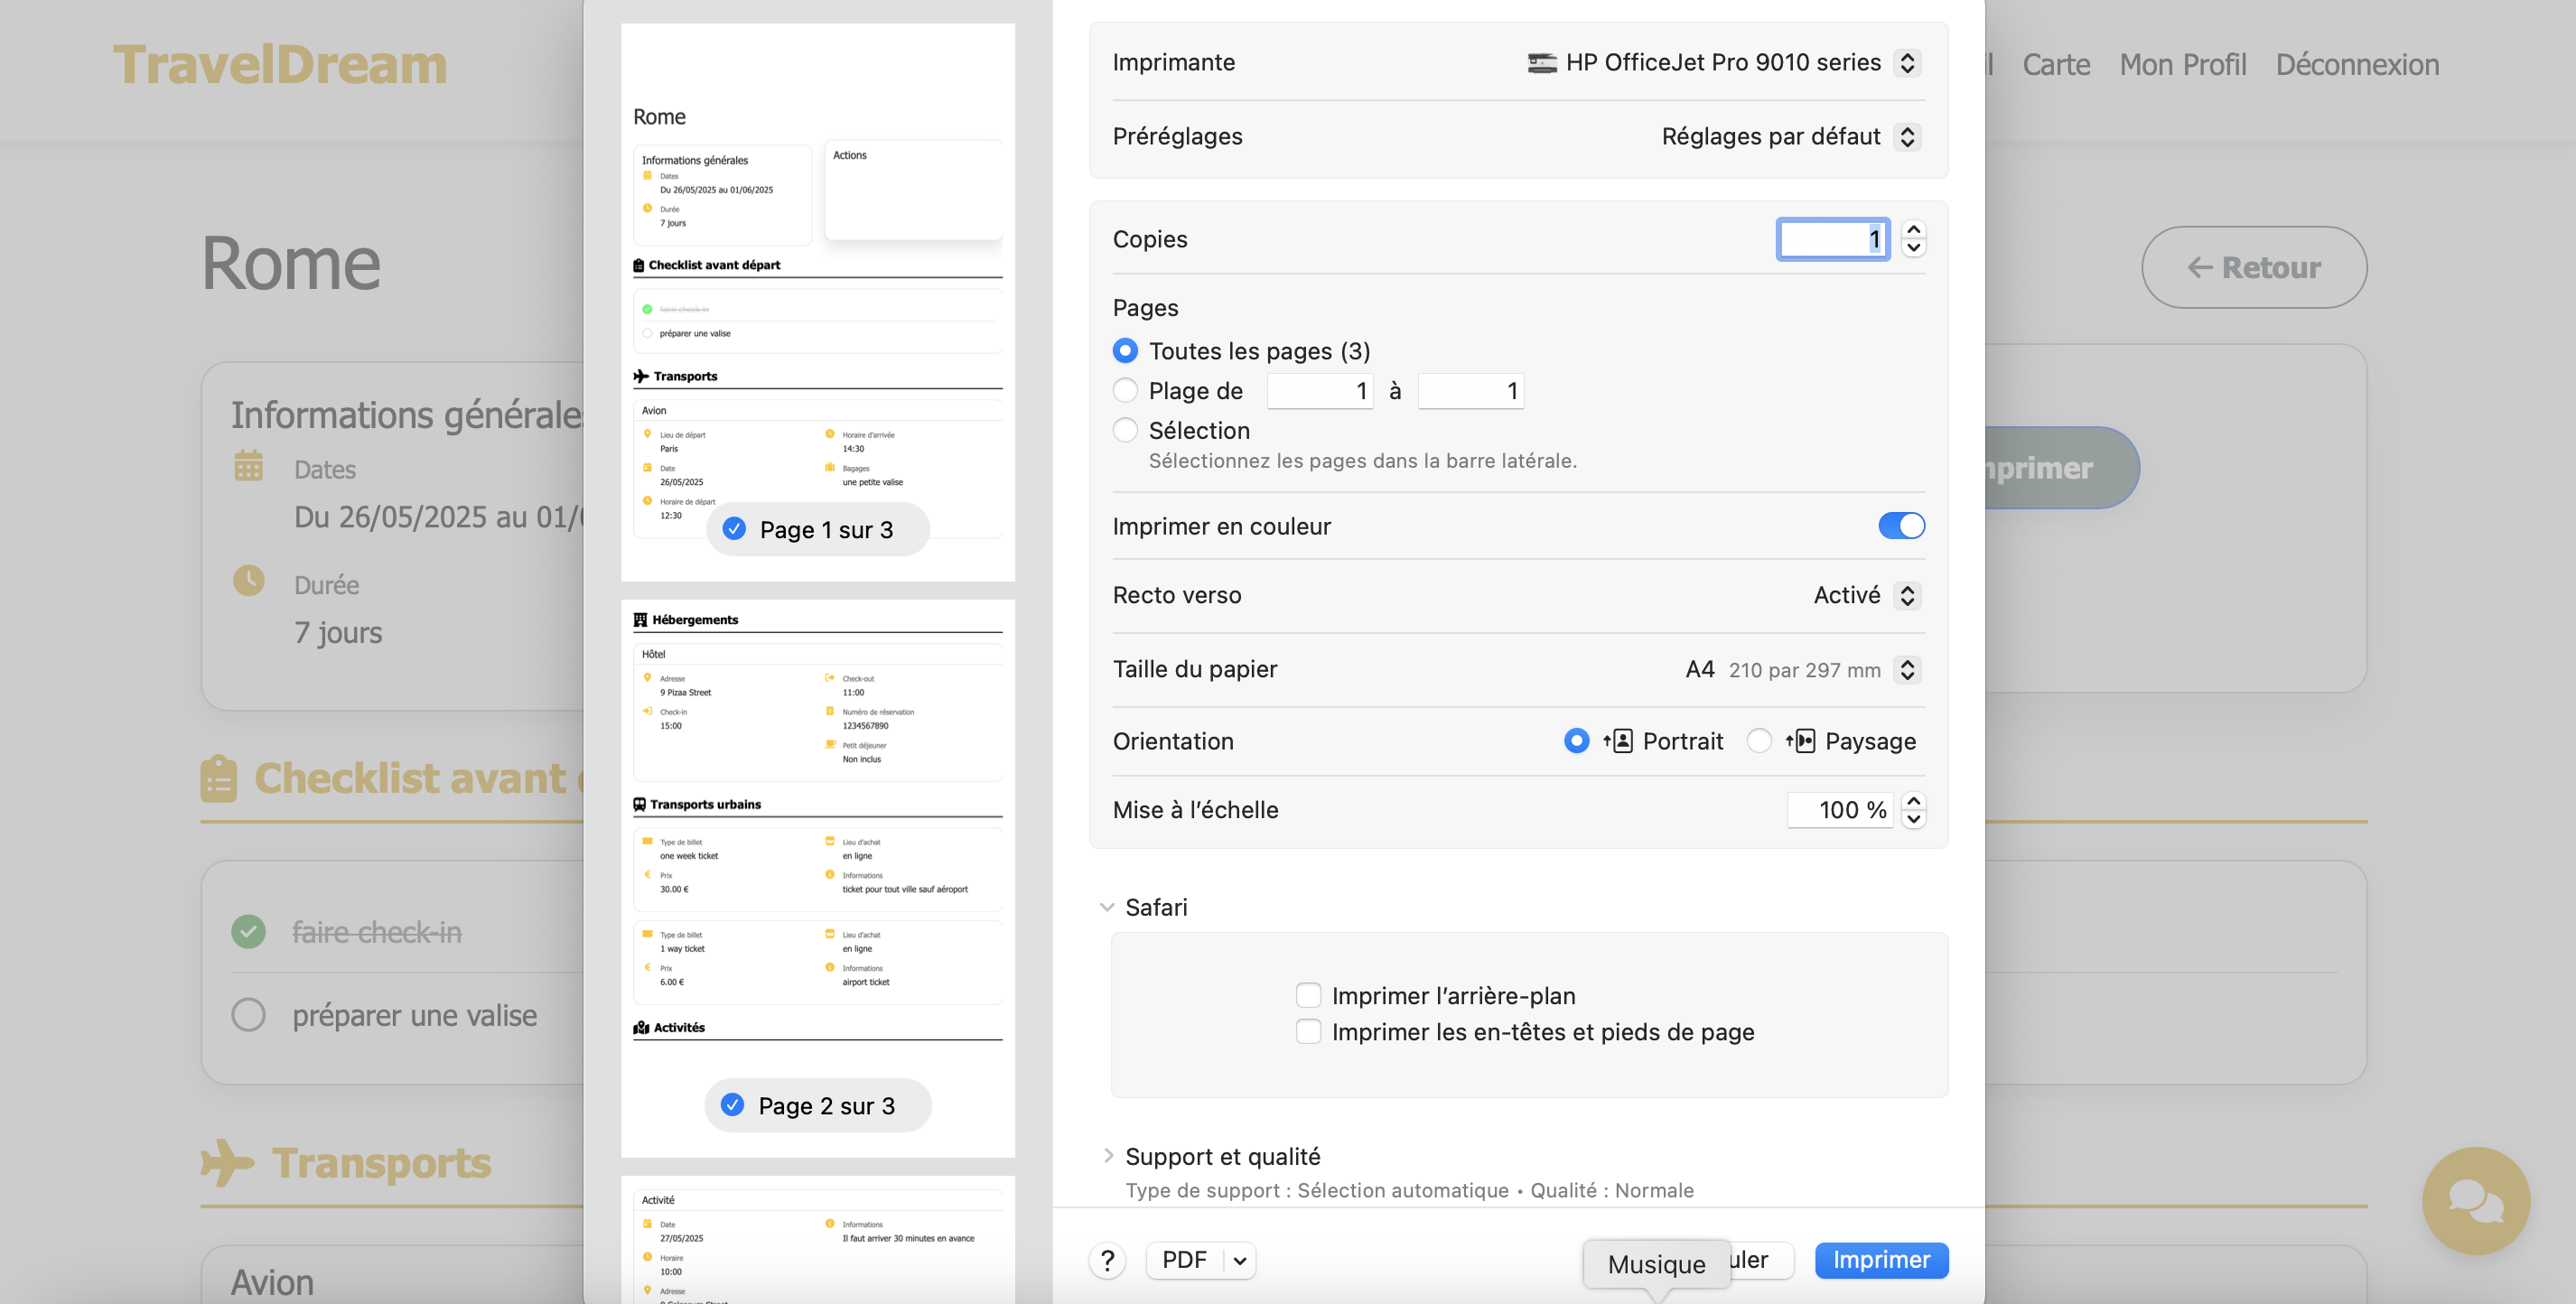
\includegraphics[width=0.8\textwidth]{11_imprimer_voyage.png}
\end{figure}



\end{document}
